\documentclass[a4paper,fleqn]{els-cas-templates/cas-sc}

\usepackage[authoryear,longnamesfirst]{natbib}
\usepackage{amsmath,amssymb}
\usepackage{booktabs}
\usepackage{multirow}
\usepackage{graphicx}
\usepackage{array}
\usepackage{placeins}
\usepackage{flafter}
\graphicspath{{./}{els-cas-templates/}}

% Keep figures and tables close to their first citation in the manuscript.
% This also protects the Overleaf build if a template copy loads endfloat.
\makeatletter
\AtBeginDocument{%
  \@ifpackageloaded{endfloat}{%
    \let\processdelayedfloats\relax
    \let\efloat@process\relax
  }{}%
}
\makeatother

\begin{document}
\let\WriteBookmarks\relax
\setcounter{topnumber}{4}
\setcounter{bottomnumber}{2}
\setcounter{totalnumber}{6}
\renewcommand{\topfraction}{0.95}
\renewcommand{\bottomfraction}{0.85}
\renewcommand{\textfraction}{0.05}
\renewcommand{\floatpagefraction}{0.75}

\shorttitle{Representation Drift in Wood Recognition}
\shortauthors{Ma--Cong and Nguyen--Trong}

\title[mode=title]{Representation Drift for Diagnosing and Monitoring\\ Wood Species Recognition Failures\\ under Acquisition Shift}

\author[1]{Thanh Ma--Cong}
\credit{Conceptualization, Methodology, Software, Formal analysis, Writing -- original draft}

\author[1,2]{Khanh Nguyen--Trong}
\cormark[1]
\ead{khanhnt@ptit.edu.vn}
\credit{Supervision, Methodology, Validation, Writing -- review and editing}

\affiliation[1]{
  organization={Intelligent Computing for Sustainable Development Lab, Posts and Telecommunications Institute of Technology (PTIT)},
  city={Hanoi},
  country={Vietnam}
}

\affiliation[2]{
  organization={Faculty of Information Technology, Posts and Telecommunications Institute of Technology (PTIT)},
  city={Hanoi},
  country={Vietnam}
}

\cortext[1]{Corresponding author: Khanh Nguyen--Trong (e-mail: khanhnt@ptit.edu.vn).}

\begin{abstract}
Computer-vision wood identification models often achieve high accuracy under controlled acquisition, but their reliability under deployment conditions remains insufficiently understood. This paper studies a specific hypothesis: recognition failures under acquisition shift are empirically associated with displacement of pretrained wood representations, and related feature-distribution displacement can be monitored without target-domain labels. We introduce MRD-Wood, a representation-drift diagnostic and monitoring protocol for frozen pretrained backbones. The main analysis links controlled perturbations to paired feature drift, validates the relationship under external datasets, separately tests cross-magnification transfer, and evaluates clean reference-bank distances as deployable monitoring signals. We also provide a margin-based analysis explaining why representation drift predicts failure and validate its per-sample prediction directly. Spatial clustering and CAM-proxy redistribution are used as secondary diagnostics to describe how failures manifest inside the representation. The study evaluates seven backbones on nine public wood dataset sources, counting VN26 as one source with three magnification subsets, using a broad suite of acquisition-shift stress tests, Tier-B validation, and cross-magnification testing. Across Tier-A perturbation experiments, paired feature drift is the strongest predictor of accuracy degradation (pooled $r=0.908$, Spearman $\rho=0.937$; partial $r=0.795$ after controlling for dataset, backbone, and perturbation family), and the relationship remains strong under grouped controls, leave-one-dataset-out validation, mixed-effects modeling, and clustered bootstrap. The same drift--accuracy relationship is corroborated on external Tier-B datasets with different acquisition pipelines and on real cross-magnification transfer, which serve as the closest available proxies for field shift. The results also reveal a robustness paradox: DINOv2-B and EfficientNet-B3 are strongest under synthetic perturbations, HRNet-32 has the highest clean accuracy, and cross-magnification accuracy drops sharply whenever VN26 magnification levels differ. For deployment monitoring, a clean reference-bank detector based on RBF-MMD reaches ROC-AUC $=0.968$ and F1 $=0.909$ in a batch-level synthetic-shift benchmark, nearly matching a paired feature-drift oracle while exposing threshold-calibration limits for unseen shift types. Overall, representation drift is the central signal of wood-identification failure under acquisition shift, and it can be monitored without target labels.
\end{abstract}

\begin{highlights}
\item Multi-dataset benchmark tests wood recognition under acquisition shifts.
\item Feature drift strongly predicts accuracy loss under controlled shifts.
\item Spatial and CAM-proxy diagnostics reveal secondary failure modes.
\item Robustness rankings are scenario-dependent, not inferred from clean accuracy.
\item Reference-bank monitoring detects deployment risk without target labels.
\end{highlights}

\begin{keywords}
wood recognition \sep acquisition shift \sep representation drift \sep spatial clustering \sep deployment monitoring
\end{keywords}

\maketitle

\section{Introduction}

Computer-vision wood identification (WoodID) is a practical pattern-recognition problem with direct implications for timber legality verification, forest-product quality control, biodiversity protection, and forensic wood inspection. In operational settings, a reliable screening system should help non-specialist users flag suspicious timber and support expert confirmation. Macroscopic computer-vision systems are attractive for this purpose because they can use portable cameras or magnifying devices and avoid the slower preparation required by microscopic analysis. Recent CNN, transformer, and patch-voting methods have therefore achieved strong clean-domain accuracy on controlled wood-image benchmarks \citep{paulafilho2014forest,sun2021smallwood,fabijanska2021woodcore,herrera2026goimai}. Field-oriented WoodID systems such as XyloTron further demonstrate why deployment reliability matters for timber screening and enforcement contexts \citep{ravindran2021field}.

However, deployment reliability is not determined by clean accuracy alone. The same wood species may be imaged under different focus quality, illumination, compression settings, sensor responses, magnifications, or specimen-preparation conditions. These changes preserve the semantic label but alter the input distribution. In WoodID, such distribution shifts are not hypothetical: recent evidence shows that digital perturbations can substantially degrade macroscopic WoodID models \citep{owens2025robustness}. This creates a gap between laboratory evaluation and field use. A model that appears accurate under a fixed acquisition protocol may fail when the acquisition protocol drifts.

Most existing WoodID studies answer the question ``which classifier is accurate?'' rather than ``why does a representation fail?'' A drop in accuracy is an endpoint; it does not reveal whether shifted samples move away from their clean feature locations, whether class geometry collapses, whether spatial representations become unstable, or whether model attention moves to different regions. This distinction is important for two reasons. First, representation-level diagnosis can identify failure mechanisms that are invisible in accuracy tables. Second, a deployable system often lacks target-domain labels, so it needs label-free signals that warn when incoming features have drifted away from a trusted clean reference distribution.

This paper addresses these issues through \textbf{MRD-Wood} (\textbf{M}onitoring \textbf{R}epresentation \textbf{D}rift for Wood Recognition), a representation-drift diagnosis and monitoring protocol for wood-recognition failures under acquisition shift. MRD-Wood does not propose another classifier. Its central claim is narrower and more testable: if a shifted image is pushed away from its clean feature neighborhood, recognition becomes less reliable; if incoming deployment features move away from a trusted clean reference bank $B_0$, the system can raise a label-free risk alert. Spatial clusters and CAM-proxy redistribution are included to interpret how the representation changes, but the main empirical bridge is feature drift. Throughout, synthetic acquisition perturbations are treated as controlled, plausible proxies for deployment shift that enable paired analysis; the degree to which they match true field shift is an empirical question, which we probe through external Tier-B datasets and cross-magnification transfer rather than assume.

The study is organized around three research questions that connect the experimental design to deployment use:

\begin{itemize}
  \item \textbf{RQ1:} How do pretrained visual backbones fail under deployment-like shifts in wood species recognition?
  \item \textbf{RQ2:} Which representation-level signals track and help explain accuracy degradation?
  \item \textbf{RQ3:} Can recognition failure be detected without target-domain labels?
\end{itemize}

The main contributions are:

\begin{enumerate}
  \item We provide a systematic robustness study of frozen pretrained backbones for WoodID across controlled perturbations, external Tier-B datasets, and cross-magnification transfer.
  \item We formulate a representation-drift diagnostic protocol that links accuracy degradation to paired feature displacement and class-geometry deformation.
  \item We give an analytical account of the phenomenon: under a frozen feature space, feature drift causes misclassification only when it crosses a sample-specific margin gate, which yields a falsifiable per-sample prediction, explains why grouped and partial correlation is the appropriate summary, and is consistent across the kNN, nearest-centroid, and linear-probe decision rules. We present this as a mechanistic explanation, not as a tight predictive bound.
  \item We show empirically that feature drift is the dominant failure signal, while spatial and CAM-proxy metrics are useful secondary diagnostics for interpreting how failure manifests.
  \item We frame the clean reference-bank monitor as a deployable label-free contribution, showing that batch monitoring can nearly match a paired feature-drift oracle in the pooled benchmark while requiring deployment-specific threshold calibration.
  \item We show that backbone robustness ranking is scenario-dependent: the best clean-accuracy model, the most perturbation-robust model, and the most magnification-transferable model differ, so deployment model selection cannot be read off clean accuracy (the ``robustness paradox'').
\end{enumerate}

Together, these results establish representation drift as the central signal of
wood-identification failure under acquisition shift, usable both as a diagnostic
principle and as a deployable monitor that requires no target-domain labels.

\section{Related Work}

\subsection{Wood species recognition and acquisition sensitivity}

Computer-vision wood identification has progressed from hand-crafted macroscopic
texture descriptors and classifier fusion \citep{paulafilho2014forest,souza2020brazilian}
to deep transfer learning, patch voting, and field-oriented systems
\citep{sun2021smallwood,fabijanska2021woodcore,degeus2021amazon,ravindran2021field}.
Public datasets and protocols such as tropical macroscopic collections,
WOOD-AUTH, GOIMAI, and magnification-level VN26 experiments further show that
wood recognition can be highly accurate under controlled acquisition while still
depending on surface preparation, scale, section, and image resolution
\citep{canosaenz2022tropical,barmpoutis2018woodauth,herrera2026goimai,nguyentrong2023magnification}.
These results establish that wood images are discriminative, but the WoodID
literature also cautions that image-level performance can overstate field utility when
data hygiene, specimen-disjoint evaluation, and acquisition conditions are not handled
carefully \citep{hermanson2011review,ravindran2022caveat}. Representative
quantitative context is summarized in Appendix Table~\ref{tab:related_quant};
the values are not directly comparable because datasets and protocols differ.

\subsection{Robustness and deployment shift}

Deployment shift is the central unresolved issue for field WoodID. ImageNet-C and domain
generalization work show that clean accuracy is not a sufficient proxy for
robustness and that claims can be protocol-sensitive
\citep{hendrycks2019corruptions,ganin2016domain,sun2016coral,gulrajani2021domainbed}.
In WoodID, \citet{owens2025robustness} explicitly reframed evaluation around
field-like perturbations, finding that resizing, blue-channel shifts, and large
blur regions can substantially damage a Peruvian WoodID model. We build on that
robustness perspective without treating our channel-shift results as a
replication or refutation: datasets, models, decision rules, and color-shift
definitions differ. The broader question addressed here is how frozen pretrained
wood representations deform when the tested acquisition shifts are expanded
across backbone families, dataset sources, optical/digital/noise/photometric
stressors, compound conditions, and magnification transfer. Prior WoodID
robustness studies typically report accuracy under selected stressors; they leave
open whether the representation itself remains stable and whether failures can be
detected without target labels.

\subsection{Representation analysis, monitoring, and positioning}

Representation analysis and deployment monitoring provide the missing diagnostic
layer. Feature geometry links accuracy to class separability and margin structure
\citep{kornblith2019representations}, while WoodID's spatial nature motivates
patch-based processing and cautious visual explanations
\citep{selvaraju2020gradcam,bai2021explainable}. OOD and monitoring methods
compare incoming features with clean reference features using confidence,
kNN/centroid distances, Mahalanobis distance, density estimates, or kernel
two-sample tests \citep{hendrycks2017baseline,lee2018mahalanobis,sun2022knn,gretton2012mmd}.
MRD-Wood integrates these ingredients into one robustness study: paired feature
drift is treated as an oracle diagnostic for controlled clean--shifted pairs,
spatial/CAM-proxy summaries describe secondary failure modes, and clean
reference-bank distances provide a deployable label-free monitor when paired
clean images and target labels are unavailable. Unlike generic OOD detectors, the
monitor is evaluated against acquisition-shift-induced WoodID failure and tied to
the representation-drift mechanism tested in the controlled experiments.
Table~\ref{tab:positioning}
summarizes this positioning.

\begin{table}[pos=htbp]
\centering
\caption{Positioning of MRD-Wood relative to representative WoodID and robustness studies. A check mark denotes an explicit component of the evaluation protocol; ``partial'' denotes limited shift-oriented evaluation that does not include the full component; ``patch'' denotes spatial patch processing rather than representation/CAM-proxy drift analysis.}
\label{tab:positioning}
\scriptsize
\setlength{\tabcolsep}{2.5pt}
\begin{tabular}{p{0.26\linewidth}cccccc}
\toprule
Study & Multi-data & Robustness & Repr. drift & Spatial/CAM-proxy & Cross-mag. & Monitor \\
\midrule
\citet{paulafilho2014forest}, \citet{souza2020brazilian} & -- & -- & -- & -- & -- & -- \\
\citet{sun2021smallwood}, \citet{fabijanska2021woodcore} & -- & -- & -- & -- & -- & -- \\
\citet{herrera2026goimai} & -- & -- & -- & patch & -- & -- \\
\citet{ravindran2021field}, \citet{ravindran2022caveat} & partial & partial & -- & -- & -- & -- \\
\citet{nguyentrong2023magnification} & -- & partial & -- & -- & \checkmark & -- \\
\citet{owens2025robustness} & -- & \checkmark & -- & -- & -- & -- \\
MRD-Wood & \checkmark & \checkmark & \checkmark & \checkmark & \checkmark & \checkmark \\
\bottomrule
\end{tabular}
\end{table}

\section{MRD-Wood: Representation-Drift Diagnosis and Monitoring}

MRD-Wood is designed around a simple failure chain: acquisition shift changes the image, the backbone representation drifts away from its clean reference structure, the kNN decision becomes less stable, and a deployment monitor can detect this risk by comparing incoming features against a clean reference bank. Figure~\ref{fig:mrd_framework} summarizes this logic. A clean image set and one or more shifted or deployment batches are passed through the same frozen backbone. The primary measurements are global feature drift, class-geometry deformation, and reference-bank monitoring. Spatial token clusters and CAM-proxy redistribution are retained as secondary diagnostic views: they help explain the form of representation change, but they are not the main predictive claim of the paper.

\begin{figure}[pos=htbp]
\centering
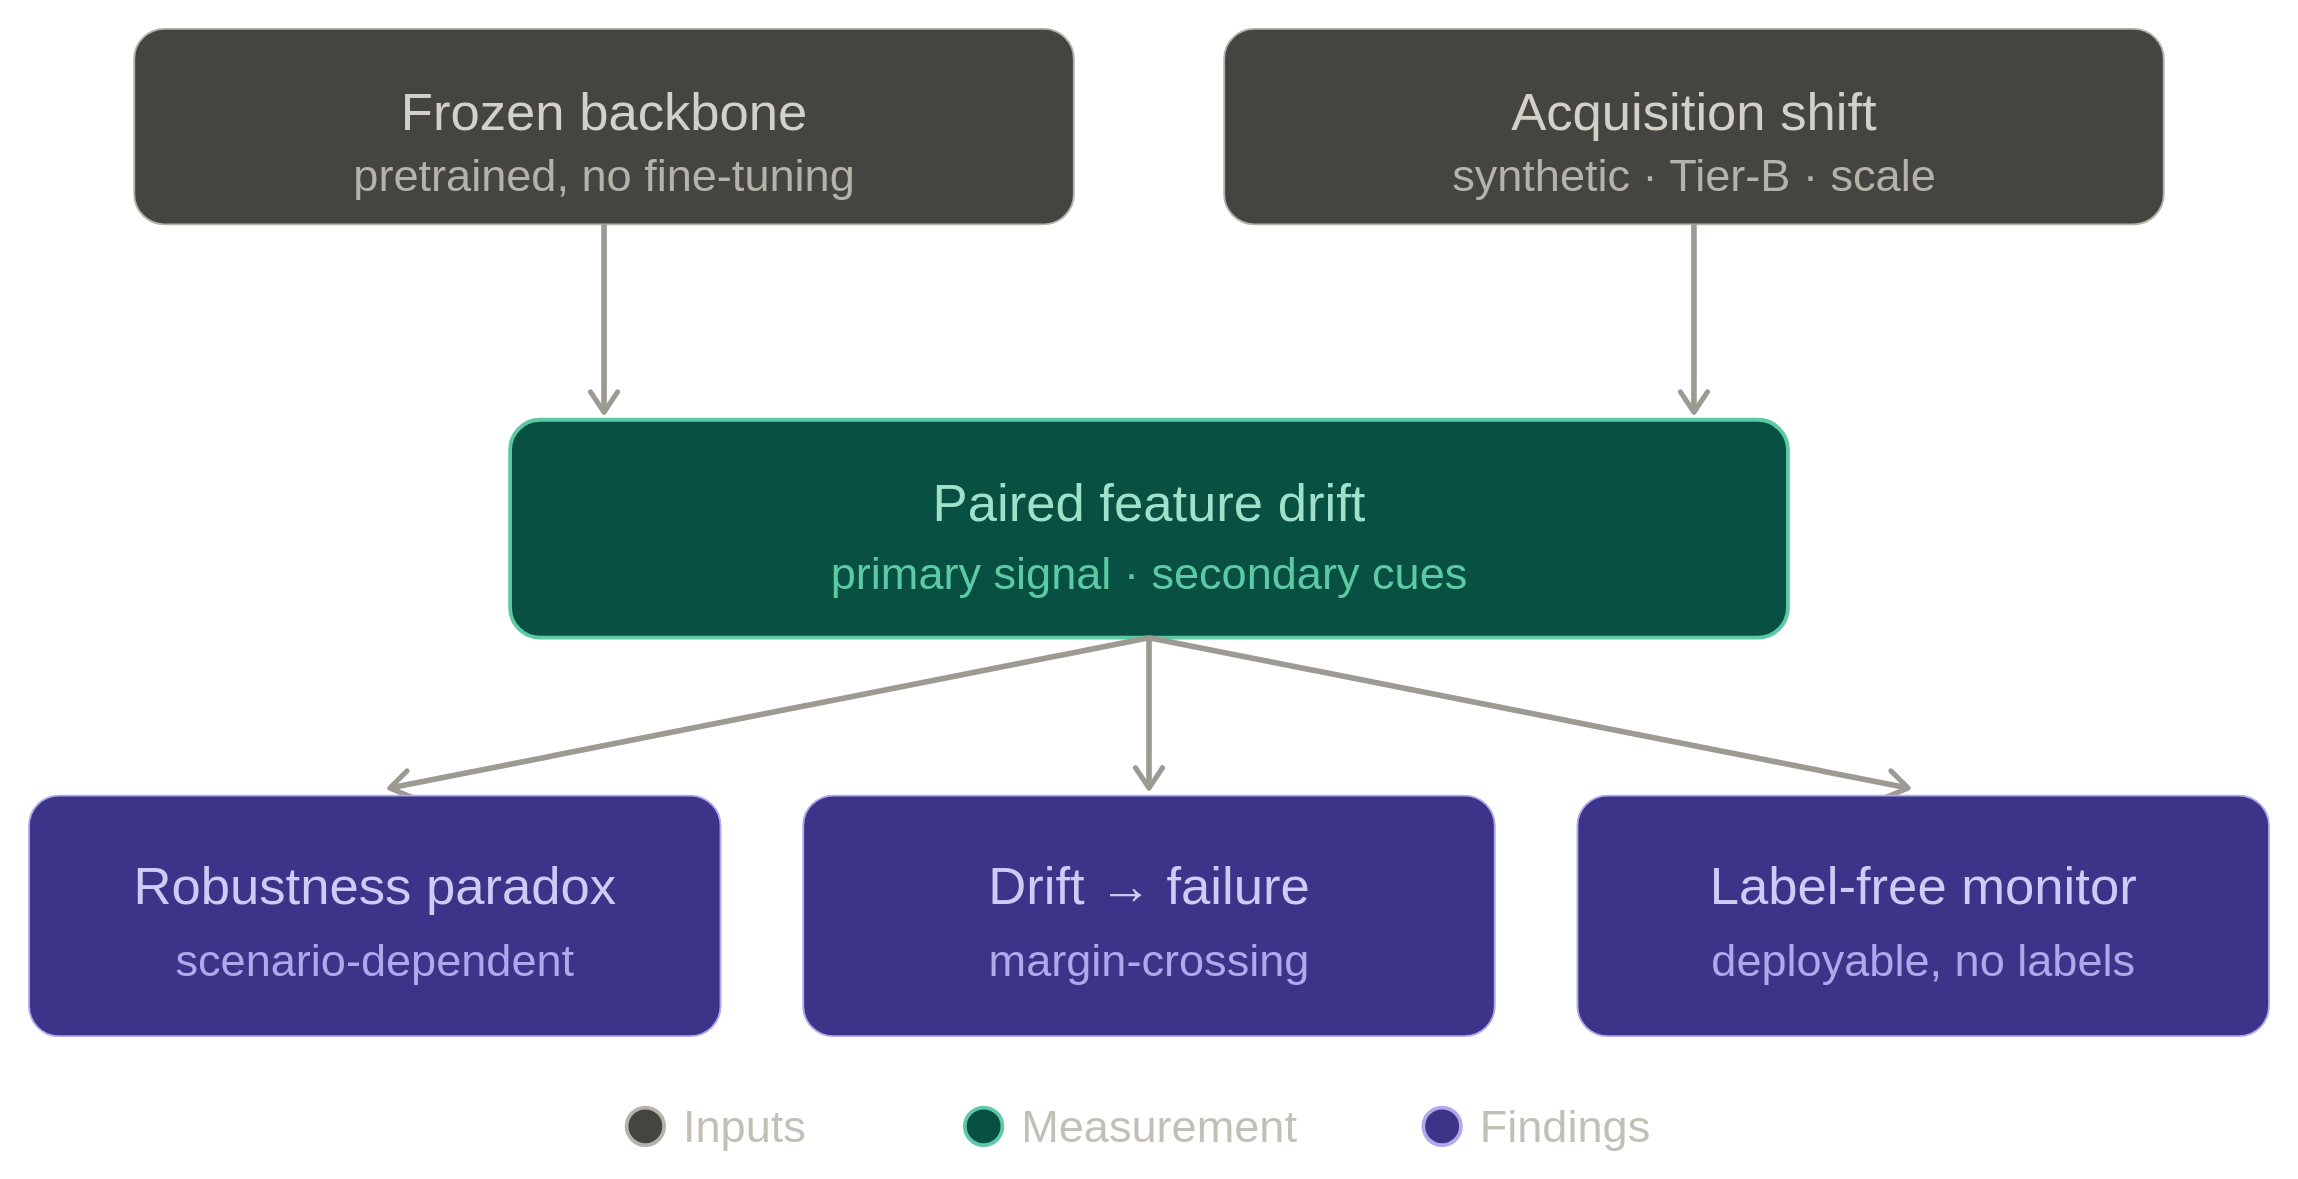
\includegraphics[width=\linewidth]{results/figures/mrd_wood_overview_figure1.png}
\caption{Overview of MRD-Wood. Frozen pretrained backbones are evaluated under acquisition shifts, paired feature drift is the primary signal, and the resulting analysis supports three outputs: scenario-dependent robustness ranking, margin-crossing explanation of failure, and label-free deployment monitoring.}
\label{fig:mrd_framework}
\end{figure}

Formally, let $D_0=\{(x_i,y_i)\}_{i=1}^{N}$ denote a clean image set and let $T_\delta$ denote an acquisition-shift operator with severity $\delta$. A shifted image is written as $x_i^\delta=T_\delta(x_i)$, and a frozen pretrained backbone maps an image to a global feature vector
\begin{equation}
  z_i = f_\theta(x_i), \qquad \hat{z}_i = \frac{z_i}{\|z_i\|_2}.
\end{equation}
Normalizing to the unit sphere makes all subsequent geometry depend on direction rather than magnitude, matching the cosine decision rule. The normalized features extracted from $D_0$ form the clean reference bank $B_0$ used for deployment monitoring.
The decision-level degradation is measured by the accuracy drop
\begin{equation}
  \Delta A_\delta = A_0 - A_\delta,
\end{equation}
where $A_0$ and $A_\delta$ are the clean and shifted accuracies.

For reference, the symbols used in the diagnostic protocol are as follows.
Each image is mapped to a global, $L_2$-normalized feature $\hat z$; $\Delta_f$
denotes the paired feature drift between a clean image and its shifted
counterpart; $d_{\mathrm{intra}}$ and $d_{\mathrm{inter}}$ denote intra-class
compactness and inter-class separation, summarized by the feature-geometry
collapse score $FGCS$. At the spatial level, $SGI$ measures the granularity of
the clustered token map and $CSI$ (with its permutation-invariant variant
$CSI_H$) measures spatial-cluster stability under shift. At the activation
level, $H(p)$ and $JSD$ measure, respectively, the concentration and the
clean-to-shift redistribution of a centroid activation map (CAM-proxy). Finally,
$B_0$ denotes the clean reference bank of features used for label-free
deployment monitoring and $B_t$ an incoming deployment batch. Lower-case $r$ and
$\rho$ denote Pearson and Spearman correlations; the statistical conventions are
detailed in Section~\ref{sec:quant_protocol}.

\subsection{Global feature drift and class geometry}
\label{sec:global_drift}

The primary signal of MRD-Wood is whether a perturbed image still maps close to
its own clean location in the feature space that the classifier actually uses.
For controlled perturbation experiments, where a clean image and its shifted
counterpart are both available, paired feature drift is defined as the cosine
displacement between the two embeddings:
\begin{equation}
  \Delta_f(x_i,\delta)
  = 1 -
  \frac{f_\theta(x_i)^\top f_\theta(T_\delta(x_i))}
  {\|f_\theta(x_i)\|_2\,\|f_\theta(T_\delta(x_i))\|_2}.
\end{equation}
A value of $0$ means the perturbation did not move the representation at all,
while larger values mean the shifted feature points in an increasingly different
direction. This quantity is an \emph{oracle} diagnostic because it requires a
clean--shifted image pair, which is unavailable at deployment; it is used here
only to test whether representation displacement is empirically linked to
recognition failure.

Beyond the movement of individual samples, we also characterize how the overall
class structure deforms. For each class $c$, the class centroid summarizes the
typical clean location of that class on the unit sphere,
\begin{equation}
  \mu_c=\frac{1}{|D_c|}\sum_{x_i\in D_c}\hat{z}_i ,
\end{equation}
and the within- and between-class structure is summarized by intra-class
compactness and inter-class separation,
\begin{equation}
  d_{\mathrm{intra}}=
  \frac{1}{C}\sum_{c=1}^{C}\frac{1}{|D_c|}
  \sum_{x_i\in D_c}\|\hat{z}_i-\mu_c\|_2 ,
\end{equation}
\begin{equation}
  d_{\mathrm{inter}}=
  \frac{2}{C(C-1)}\sum_{i<j}\|\mu_i-\mu_j\|_2 .
\end{equation}
Intuitively, $d_{\mathrm{intra}}$ is the average spread of samples around their
own class centre, and $d_{\mathrm{inter}}$ is the average distance between class
centres; a smaller spread and a larger centroid separation make the
nearest-neighbour decision more stable. We combine the two into a single
separability summary, the feature-geometry collapse score,
\begin{equation}
  FGCS=\frac{d_{\mathrm{inter}}}{d_{\mathrm{intra}}+\epsilon},
\end{equation}
where a higher $FGCS$ indicates a more separable feature configuration.

Because the absolute value of $FGCS$ depends on the dataset and backbone, we
report how class geometry \emph{changes} under shift rather than its level. In
particular, inter-class collapse is the reduction in mean pairwise centroid
separation,
\begin{equation}
  \Delta d_{\mathrm{inter}}
  = d_{\mathrm{inter}}^{\mathrm{clean}} - d_{\mathrm{inter}}^{\mathrm{shift}},
\end{equation}
so a \emph{positive} value means the average distance between class centroids
\emph{decreases} under shift, shrinking inter-class margins and making confusion
more likely. We stress that this is a relative contraction of the centroid
configuration, not a literal merging of all classes into a single cluster.

\subsection{Spatial clusters}
\label{sec:spatial_clusters}

The remaining diagnostic components of MRD-Wood are \emph{secondary diagnostics} that describe
\emph{how} the representation changes, not \emph{whether} it predicts failure
(that is the role of global drift, Section~\ref{sec:global_drift}). At the spatial
level we cluster the $L_2$-normalized spatial token map with KMeans
\citep{lloyd1982least} ($K{=}3$, a low-complexity diagnostic choice;
Appendix~\ref{app:spatial_cam}) and summarize it with a spatial granularity index
($SGI$, how fragmented the partition is) and a cluster-stability index ($CSI$,
with a Hungarian permutation-invariant variant $CSI_H$, how much the partition is
preserved under shift). Full definitions are given in
Appendix~\ref{app:spatial_cam}.

\subsection{CAM-proxy cluster redistribution}
\label{sec:cam_cluster}

At the activation level we use a gradient-free, centroid-based class-activation
proxy (the \emph{CAM-proxy}; a similarity-based saliency map, not a causal or
gradient method) and summarize how its activation mass is distributed over the
spatial clusters from Section~\ref{sec:spatial_clusters} by its entropy $H(p)$
and its clean-to-shift redistribution (Jensen--Shannon divergence $JSD$). Full
definitions, including the CAM-proxy map and the distribution metrics, are given
in Appendix~\ref{app:spatial_cam}.

\subsection{Reference-bank deployment monitoring}
\label{sec:refbank}

The diagnostics above all assume access to a clean--shifted pair, which a deployed
field system does not have: the operator observes only the incoming image, with no
clean version of the same sample. The monitoring level therefore replaces paired
comparison with a comparison against a fixed \emph{clean reference bank}
$B_0=\{\hat{z}_i\}_{i=1}^{N}$, against which an incoming deployment batch $B_t$ is
scored. All four monitors below answer the same question --- how far has the
incoming batch moved away from $B_0$? --- and differ only in how much of the
reference distribution they use.

The simplest monitor measures distance to the nearest clean neighbours
(point level). For an incoming image $u$, the per-sample $k$NN distance is
\begin{equation}
  s_{kNN}(u)=
  \frac{1}{k}\sum_{j\in NN_k(f_\theta(u),B_0)}
  d_{\cos}(f_\theta(u),z_j),
\end{equation}
and the monitor reports the batch mean
$S_{kNN}(B_t)=|B_t|^{-1}\sum_{u\in B_t}s_{kNN}(u)$. A coarser monitor compares
batch centroids (first-moment level),
\begin{equation}
  S_{\mathrm{centroid}}(B_t)=1-\bar{z}_0^{\top}\bar{z}_t,
  \qquad
  \bar{z}_t=\frac{\sum_{y\in B_t}\hat{z}_y}{\|\sum_{y\in B_t}\hat{z}_y\|_2},
\end{equation}
where $\bar z_0$ is the clean reference-bank centroid. A covariance-aware monitor
rescales the distance to the reference mean by the clean feature covariance
(second-moment level), using a Ledoit--Wolf estimator \citep{ledoit2004well} for
$\Sigma_0$,
\begin{equation}
  S_M(B_t)=\frac{1}{|B_t|}\sum_{y\in B_t}
  (\hat{z}_y-\mu_0)^{\top}\Sigma_0^{-1}(\hat{z}_y-\mu_0).
\end{equation}
Finally, the most distributional monitor compares the whole incoming batch to the
reference bank with a kernel two-sample statistic, the RBF maximum mean
discrepancy between $B_0=\{a_i\}_{i=1}^{n}$ and $B_t=\{b_j\}_{j=1}^{m}$,
\begin{equation}
  \widehat{MMD}^2(B_0,B_t)=
  \frac{1}{n^2}\sum_{i,j} k(a_i,a_j)
  +\frac{1}{m^2}\sum_{i,j} k(b_i,b_j)
  -\frac{2}{nm}\sum_{i,j} k(a_i,b_j),
\end{equation}
where $k(a,b)=\exp(-\gamma\|a-b\|_2^2)$ and $\gamma$ is set by a median-distance
heuristic on the compared feature batches; $\widehat{MMD}^2$ is small when the two
feature distributions coincide and grows as they diverge. All four monitors
require only the clean reference bank $B_0$ and use \emph{no labels} for the
incoming batch, which is what makes them deployable.

\subsection{Analytical account: why representation drift predicts failure}
\label{sec:analytical}

The preceding metrics are empirical descriptors. This subsection gives the
analytical reason a single descriptor --- paired feature drift --- predicts
recognition failure, so that the experiments in
Section~\ref{sec:results_drift} can be read as confirming a stated mechanism
rather than reporting an unexplained correlation. We stress that this is a
conservative mechanistic account rather than a tight predictive law: the bound
is worst-case (Section~\ref{sec:results_drift} shows it certifies only a small
fraction of samples), and its role is to explain \emph{why} drift tracks
failure, not to improve prediction over drift itself. The argument does not require
any assumption about the black-box backbone $f_\theta$; it is a property of the
\emph{decision geometry} induced on the unit sphere by a frozen feature space,
treated as fixed points together with a known decision rule. Throughout, a
sample $x$ has true label $y$ and normalized clean feature $\hat z$, and its
shifted counterpart has feature $\hat z'$ with paired drift
$\Delta_f = 1-\langle \hat z,\hat z'\rangle$.

\paragraph{A geometric identity.}
Because features are $L_2$-normalized, cosine drift is exactly a squared
Euclidean displacement on the sphere.

\noindent\textbf{Lemma 1 (drift--displacement identity).}
\emph{For unit vectors $\hat z,\hat z'$,
$\;\|\hat z'-\hat z\|_2 = \sqrt{2\,\Delta_f}\,$.}

\noindent\emph{Proof.}
$\|\hat z'-\hat z\|_2^2 = \|\hat z'\|_2^2+\|\hat z\|_2^2-2\langle \hat z,\hat z'\rangle
= 2-2(1-\Delta_f)=2\Delta_f$. \hfill$\square$

\paragraph{Drift erodes the classification margin.}
Consider the prototype (cosine nearest-centroid) rule used as one of the
decision rules in Appendix~\ref{app:additional_checks}: with class prototypes
$p_c=\mu_c/\|\mu_c\|_2$, a feature is assigned to
$\arg\max_c \langle \hat z,p_c\rangle$. For a correctly classified clean sample,
define the clean margin
\begin{equation}
  \Gamma(x)=\langle \hat z,p_y\rangle-\max_{c\neq y}\langle \hat z,p_c\rangle>0 .
  \label{eq:margin}
\end{equation}

\noindent\textbf{Lemma 2 (the margin is $2$-Lipschitz).}
\emph{$\;|\Gamma(\hat z')-\Gamma(\hat z)|\le 2\,\|\hat z'-\hat z\|_2\,$.}

\noindent\emph{Proof.}
Each score $\hat z\mapsto\langle \hat z,p_c\rangle$ is $1$-Lipschitz since
$\|p_c\|_2=1$. A pointwise maximum of $1$-Lipschitz functions is $1$-Lipschitz,
so $\max_{c\neq y}\langle\cdot,p_c\rangle$ is $1$-Lipschitz; $\Gamma$ is a
difference of two $1$-Lipschitz functions and is therefore $2$-Lipschitz.
\hfill$\square$

\noindent\textbf{Proposition 1 (label preservation under bounded drift).}
\emph{If $x$ is correctly classified with margin $\Gamma(x)$ and}
\begin{equation}
  \Delta_f(x) < \frac{\Gamma(x)^2}{8},
  \label{eq:preserve}
\end{equation}
\emph{then $x^\delta$ is also correctly classified.}

\noindent\emph{Proof.}
By Lemma 2 and Lemma 1,
$\Gamma(\hat z')\ge \Gamma(\hat z)-2\|\hat z'-\hat z\|_2
=\Gamma(x)-2\sqrt{2\Delta_f}$. If $\Delta_f<\Gamma(x)^2/8$ then
$2\sqrt{2\Delta_f}<2\sqrt{2\cdot\Gamma(x)^2/8}=\Gamma(x)$, hence
$\Gamma(\hat z')>0$ and the shifted feature keeps the correct label.
\hfill$\square$

\noindent\textbf{Corollary 1 (drift is necessary but not sufficient for failure).}
\emph{A previously correct sample can be misclassified only if}
\begin{equation}
  \Delta_f(x)\ \ge\ \frac{\Gamma(x)^2}{8}.
  \label{eq:necessary}
\end{equation}

Corollary~\ref{eq:necessary} is the mechanism behind the empirical result.
Failure is gated by a sample-specific threshold $\Gamma(x)^2/8$: a large drift in
a wide-margin region need not flip the label, while a small drift near a decision
boundary can. This is exactly why feature drift is a strong but imperfect
predictor of failure, and it makes the relationship non-tautological even though
drift is measured in the same space the classifier uses --- a continuous
displacement is converted into an error only after it crosses the margin gate
of Eq.~\eqref{eq:necessary}.

\paragraph{The same law holds for other decision rules.}
The bound is not specific to the prototype rule. For a frozen linear probe with
class weights $\{w_c\}$ and scores $g_c(\hat z)=w_c^\top\hat z+b_c$, each score is
$\|w_c\|_2$-Lipschitz, so with $L=2\max_c\|w_c\|_2$ the analogous condition is
$\Delta_f(x)\ge \Gamma_{\mathrm{lin}}(x)^2/(2L^2)$, where $\Gamma_{\mathrm{lin}}$
is the linear score margin. The functional form is identical; only the
rule-dependent constant changes. This explains why the kNN, nearest-centroid, and
linear-probe results in Appendix~\ref{app:additional_checks} all exhibit the same
strong drift/drop association: they are three instances of one margin law, not
three independent coincidences. For the $k$NN rule the same logic holds with a
\emph{local} margin (the gap between the query's distances to the nearest
same-class and nearest different-class gallery points), so a flip again requires
drift large enough to reorder these neighbours.

\paragraph{From per-sample bound to group-level accuracy drop.}
Proposition 1 is a statement about individual samples; the reported quantity is a
group-level accuracy drop. The sufficient condition in Eq.~\eqref{eq:preserve}
also gives its contrapositive failure gate. Fix a group $G$ (a
dataset--backbone pair) and write
$\tau(x)=\Gamma(x)^2/8$ for the per-sample failure threshold. Under the
first-crossing model in which a previously correct sample fails exactly when its
drift exceeds its threshold (the sharp-margin version of
Corollary~\ref{eq:necessary}), the group accuracy drop is
\begin{equation}
  \Delta A(G)=\Pr_{x\in G}\!\left[\Delta_f(x)\ge \tau(x)\right].
  \label{eq:groupdrop}
\end{equation}

\noindent\textbf{Proposition 2 (monotonicity and the role of grouped controls).}
\emph{Within a group whose margin distribution (hence the law of $\tau$) is fixed,
if increasing perturbation severity increases per-sample drift in the usual
stochastic order, then $\Delta A(G)$ in Eq.~\eqref{eq:groupdrop} is
non-decreasing in severity.}

\noindent\emph{Proof.}
For each fixed threshold value $t$, $s\mapsto\Pr[\Delta_f\ge t]$ is non-decreasing
when the drift distribution increases in stochastic order. Equation~\eqref{eq:groupdrop}
is the mixture of these probabilities over the fixed law of $\tau$, and a mixture
of non-decreasing functions is non-decreasing. \hfill$\square$

Proposition 2 explains the precise pattern observed in
Section~\ref{sec:results_drift}. \emph{Within} a group the margin distribution is
fixed, so accuracy drop is a monotone functional of the drift distribution and the
within-group drift/drop association is high (Table~\ref{tab:consistency}).
\emph{Across} groups the margin distribution itself varies --- different backbones
and datasets place class boundaries differently --- which injects between-group
variance and attenuates the pooled correlation. Removing exactly this
between-group margin variation is what the partial correlation does, which is why
the partial coefficient ($r=0.795$) is the mechanistically honest summary and the
pooled coefficient ($r=0.908$) is an upper-bound mixture. The theory therefore
predicts the ordering pooled $\ge$ partial and high within-group consistency,
both of which are observed.

\paragraph{Principled reading of the auxiliary metrics.}
The remaining metrics inherit well-defined properties that make them diagnostic
rather than ad hoc. (i) The feature-geometry collapse score is invariant to any
global orthogonal transform $Q\in O(d)$ of the feature space: $Q$ preserves every
pairwise Euclidean distance entering $d_{\mathrm{intra}}$ and $d_{\mathrm{inter}}$,
so $FGCS$ depends on intrinsic class geometry, not on the coordinate frame; this
is why only its \emph{change} under shift, $\Delta d_{\mathrm{inter}}$, is
reported. (ii) The Hungarian spatial-stability index $CSI_H$ is invariant to
relabelling of the shifted clusters by construction of the $\max_\pi$ over
permutations, which is the formal justification for Hungarian matching. (iii) The
CAM-proxy satisfies $M\in[0,1]$ by min--max normalization, its cluster
distribution entropy satisfies $H(p)\in[0,\log K]$, and the redistribution score
satisfies $JSD\in[0,\log 2]$ with $JSD=0$ if and only if the clean and shifted
allocations coincide; the extremes therefore have a definite meaning (no
redistribution versus maximal redistribution).

\paragraph{The deployment monitors form a moment hierarchy.}
The four monitors of Section~\ref{sec:refbank} are not an arbitrary menu but a
nested sequence in the moments of the feature distribution they compare against
the clean reference bank $B_0$. With a linear kernel $k(a,b)=a^\top b$, the
maximum mean discrepancy reduces to a difference of means,
$\widehat{MMD}^2=\|\bar a-\bar b\|_2^2$; for the $L_2$-normalized batch means used
here this equals $2\,S_{\mathrm{centroid}}$, so the centroid monitor is exactly
the first-moment (linear-kernel) special case of MMD. The Mahalanobis monitor adds
second-moment (covariance) information, and the RBF kernel is
\emph{characteristic}, so its population MMD vanishes if and only if the two
feature distributions are identical \citep{gretton2012mmd}, capturing all
moments. Choosing among the monitors is thus a bias--variance and compute
trade-off along a single moment hierarchy (mean $\subset$ mean$+$covariance
$\subset$ full distribution), which is consistent with the RBF-MMD monitor being
the strongest detector in Section~\ref{sec:monitoring_results}.

\paragraph{A falsifiable prediction.}
Corollary~\ref{eq:necessary} yields a testable, per-sample prediction that goes
beyond a pooled correlation. Define the \emph{margin-normalized drift}
\begin{equation}
  \widetilde{\Delta}_f(x)=\frac{8\,\Delta_f(x)}{\Gamma(x)^2},
  \label{eq:normdrift}
\end{equation}
so that the theory predicts failures to concentrate where
$\widetilde{\Delta}_f(x)\ge 1$. The normalization in Eq.~\eqref{eq:normdrift}
therefore converts raw drift into a margin-relative crossing score. Two
consequences are checked in Section~\ref{sec:results_drift}: (a) among samples
that flip, the necessary condition $\Delta_f\ge\Gamma^2/8$ should hold up to
estimation noise; and (b) whether the margin against the clean nearest
competitor, evaluated at the shifted feature (Eq.~\eqref{eq:firstorder}),
identifies failures that raw drift magnitude alone does not. Because this
worst-case bound ignores the direction of the displacement, we also report a
clean-competitor margin diagnostic based on the clean nearest competing
prototype $p_{c^\ast}$,
\begin{equation}
  \widehat{\Gamma}(\hat z') =
  \Gamma(x)-\langle \hat z-\hat z',\,p_y-p_{c^\ast}\rangle,
  \label{eq:firstorder}
\end{equation}
where $c^\ast=\arg\max_{c\neq y}\langle \hat z,p_c\rangle$ is defined on the
clean feature. Expanding the inner product gives
$\widehat{\Gamma}(\hat z')=\langle \hat z',\,p_y-p_{c^\ast}\rangle$, i.e.\ the exact
margin of the true class against its clean nearest competitor evaluated at the
shifted feature. Hence $\widehat{\Gamma}(\hat z')\le 0$ is a \emph{sufficient}
condition for misclassification (the competitor $c^\ast$ has overtaken the true
class), though not a necessary one, since a third class may instead become the
winner.

\section{Experimental Design}

The experiments are designed to move from controlled failure induction to deployment-oriented validation. The first stage applies synthetic perturbations to controlled Tier-A datasets so that clean-shifted pairs are available and representation changes can be measured precisely. The second stage tests whether the same feature-drift relationships hold on additional public datasets with different acquisition histories. The third stage separately isolates magnification shift on VN26, because magnification changes alter the scale of anatomical patterns and are a common deployment risk in WoodID. Finally, the monitoring experiments ask whether failure can be detected without target labels.

\subsection{Dataset tiers and their roles}

Table~\ref{tab:datasets} summarizes the dataset tiers. Tier-A datasets (WRD25, DTSR14, PCA11) provide the main controlled perturbation setting. These datasets are used to estimate feature drift, spatial cluster changes, CAM-proxy redistribution, and accuracy drop under known perturbation severity. Tier-B datasets (BFS46, FSDM41, GOIMAI, WOODAUTH, BD11) are not used merely to enlarge the sample size; they serve as an external validity check, because their acquisition procedures, species composition, and image characteristics differ from Tier-A. Tier-C corresponds to VN26 at three magnification levels, enabling a separate analysis of scale shift that cannot be reduced to blur or compression alone.

\begin{table}[pos=htbp]
\centering
\caption{Dataset organization used in the study. Image counts refer to the curated image sets used in the experiments.}
\label{tab:datasets}
\scriptsize
\begin{tabular}{p{0.09\linewidth}p{0.13\linewidth}rrp{0.28\linewidth}p{0.23\linewidth}}
\toprule
Tier & Dataset & Classes & Images & Acquisition summary & Role \\
\midrule
Tier-A & WRD25 & 25 & 2167 & Smartphone through 20$\times$ magnifying glass & Main perturbation analysis \\
Tier-A & DTSR14 & 14 & 8903 & Flatbed-scanned wood-core RGB patches & Main perturbation analysis \\
Tier-A & PCA11 & 11 & 10795 & Digital magnifying glass, 640$\times$480 & Main perturbation analysis \\
Tier-B & BFS46 & 46 & 1901 & Zeiss stereomicroscope, 10$\times$ & External validation \\
Tier-B & FSDM41 & 41 & 2942 & Macro box with controlled halogen illumination & External validation \\
Tier-B & GOIMAI & 37 & 2121 & Smartphone with 24$\times$ optical magnifying lens & External validation \\
Tier-B & WOODAUTH & 12 & 8561 & DSLR images cropped to 400$\times$400 & External validation \\
Tier-B & BD11 & 11 & 440 & Low-cost portable microscope and smartphone & External validation \\
Tier-C & VN26 x10/x20/x50 & 26 & 7800 & Same species set at three magnification levels & Cross-magnification analysis \\
\bottomrule
\end{tabular}
\end{table}

\subsection{Backbone and perturbation selection}

We evaluate seven frozen pretrained backbones chosen to cover complementary architectural biases: a standard residual CNN (ResNet-50 \citep{he2016resnet}), an efficient scaled CNN (EfficientNet-B3 \citep{tan2019efficientnet}), a modern ConvNet (ConvNeXt-T \citep{liu2022convnext}), a hierarchical transformer (Swin-T \citep{liu2021swin}), a self-supervised foundation-style visual representation (DINOv2-B \citep{oquab2023dinov2}), a high-resolution representation network (HRNet-32 \citep{sun2019hrnet}), and a mobile architecture (MobileNetV3 \citep{howard2019mobilenetv3}). They are intentionally kept frozen. This isolates the robustness of pretrained representations and avoids conflating the analysis with supervised adaptation or fine-tuning choices.

The perturbation families are selected to approximate common acquisition failures in macroscopic WoodID. Owens-style shifts such as blur, resize, channel shift, and scratches are included because they represent known field risks, while additional stressors cover focus/optical degradation, digital compression and pixelation, sensor noise, photometric variation, rotation, and compound field-like degradation. ImageNet-C motivates the general principle of testing diverse corruptions, but this suite is not intended as a one-to-one ImageNet-C reproduction. The goal is not to claim that these perturbations exhaust all field conditions, but to create controlled, reproducible stressors that can be linked to representation-level changes.

Table~\ref{tab:severity} gives the exact severity values used to generate the cached features. Perturbations are applied to denormalized RGB tensors after resizing to the model input size and before ImageNet renormalization. Resize perturbation is implemented as a center zoom followed by bilinear resizing back to the input size; defocus blur uses a disk-shaped point-spread kernel; JPEG uses encode/decode simulation; color and illumination changes are clipped to the valid RGB range; and rotation uses the standard torchvision rotation operator. The compound presets combine Gaussian blur, brightness scaling, and JPEG compression. These values define the experimental stress test and should be interpreted as controlled acquisition proxies rather than a complete model of all field degradations.

\begin{table}[pos=htbp]
\centering
\caption{Perturbation severities used in the controlled robustness benchmark.}
\label{tab:severity}
\small
\begin{tabular}{lp{0.66\linewidth}}
\toprule
Perturbation family & Severity values \\
\midrule
Blur/focus & Gaussian blur $\sigma=\{2,4,6,8,10,12\}$; defocus radius $\{3,5,8,11,15\}$; motion blur $\{5,9,15\}$; zoom blur $\{1.05,1.10,1.20\}$ \\
Geometric/scale & Resize factors $\{1.33,1.67,2.00\}$; rotations $\{45^\circ,90^\circ,135^\circ,180^\circ\}$ \\
Photometric/channel & Illumination factors $\{0.70,0.85,1.15,1.30\}$; contrast factors $\{0.50,0.75,1.25,1.50\}$; RGB-channel offsets $\{-45,-30,30,45\}$ \\
Digital/noise & JPEG quality $\{10,20,30,50,70\}$; pixelation $\{0.50,0.33,0.25\}$; Gaussian noise $\{0.02,0.05,0.10\}$; shot noise $\{60,30,15\}$; impulse noise $\{0.01,0.03,0.05\}$ \\
Surface/compound & Scratch severity $\{\text{mild},\text{moderate},\text{severe}\}$; compound, compound-optical, compound-digital, and compound-field presets at mild/moderate/severe levels \\
\bottomrule
\end{tabular}
\end{table}

\subsection{Frozen-feature recognition protocol}

All reported accuracies are computed on frozen feature extractors rather than on fine-tuned WoodID classifiers. For each backbone, the classifier head is removed, global pooled features are L2-normalized, and a cosine 5-nearest-neighbor decision rule is used. Clean accuracy is estimated with five stratified shuffle splits using an 80/20 train/test split within each dataset. The split is stratified at the image-file level because specimen-level metadata are not consistently available across all public datasets; therefore, clean accuracy is interpreted as a representation-separability benchmark rather than as a specimen-disjoint deployment estimate. Perturbation accuracy uses a paired gallery--query stability protocol: clean features form the labeled gallery and the corresponding perturbed features form the query set. This protocol deliberately asks whether a shifted image remains compatible with the clean feature distribution of the same acquisition set; it should therefore be interpreted as a representation-stability benchmark rather than as a specimen-disjoint deployment estimate. To reduce dependence on one decision rule, Appendix~\ref{app:additional_checks} reports kNN sensitivity, nearest-centroid classification, and a frozen linear-probe check.

The same distinction is used in external and monitoring experiments. Tier-B experiments reuse the frozen-feature kNN protocol to test whether the drift/drop relationship persists under different acquisition histories, while VN26 reuses the protocol to isolate magnification-level transfer. In the monitoring experiment, labels are used only to define retrospective failure labels for evaluation; the deployed monitor scores incoming features against a clean reference bank without using target labels. The main results use $k=5$ following a conservative local-voting protocol; Appendix~\ref{app:additional_checks} verifies that the drift/drop conclusion is stable for $k\in\{1,3,5,10\}$ and for nearest-centroid classification.

\subsection{Experiment groups}

Table~\ref{tab:experiment_map} summarizes the analytical role of each experiment group. MRD-Wood is not a single metric; it is a sequence of tests that first establishes the failure phenomenon, then examines representation-level changes, then checks external validity, and finally evaluates deployment monitoring.

\begin{table}[pos=htbp]
\centering
\caption{Experimental design and analytical role of each experiment group.}
\label{tab:experiment_map}
\footnotesize
\begin{tabular}{p{0.16\linewidth}p{0.39\linewidth}p{0.35\linewidth}}
\toprule
Group & Analytical role & Reported analyses \\
\midrule
Robustness & Measure accuracy changes under controlled acquisition shifts & Accuracy matrix, severity curves, backbone ranking \\
Feature geometry & Relate representation displacement and class-geometry deformation to failure & Feature drift, intra/inter-class change, FGCS \\
Spatial/CAM-proxy & Characterize spatial organization and activation allocation under shift & SGI, CSI, CAM-proxy entropy, CAM-JSD \\
Generalization & Test feature-drift generality beyond Tier-A and separately evaluate magnification shift & Tier-B validation, VN26 cross-magnification \\
Synthesis/monitoring & Quantify incremental explanatory value and label-free detection & Hierarchical $R^2$, partial correlations, reference-bank AUC \\
\bottomrule
\end{tabular}
\end{table}

\subsection{Quantitative protocol and statistical analysis}
\label{sec:quant_protocol}

Quantitative experiments use the standard cached-feature protocol. Images are resized to the input resolution specified by each pretrained backbone configuration (EfficientNet-B3 uses 300$\times$300; the other backbones use 224$\times$224) and normalized with ImageNet statistics. Global features are extracted from timm pretrained models with the classifier removed and L2-normalized after pooling. Spatial features use timm \texttt{features\_only} with \texttt{out\_indices=(2,)} for CNN/HRNet/Swin backbones, while DINOv2-B uses intermediate ViT tokens from block 6. Spatial clustering uses $K=3$, L2-normalized spatial tokens, KMeans with ten initializations, and no PCA. This choice keeps the spatial metrics consistent with the features used in the accuracy and drift analyses. Cluster labels are brightness-ordered only for visualization. Quantitative cluster comparison uses Hungarian matching to reduce permutation ambiguity. The CAM-proxy analysis uses the centroid activation map defined in Section~\ref{sec:cam_cluster}. High-resolution VN26 figures are used only for qualitative visualization of spatial clusters and CAM-proxy overlays; they are not used as the main quantitative protocol. The robustness protocol uses five stratified shuffle splits and the global random seed is 42. The implementation requires PyTorch, torchvision, timm, scikit-learn, scipy, statsmodels-compatible mixed-effects tooling, pandas, NumPy, OpenCV, Pillow, and scikit-image; feature caches were generated with the Colab L4 configuration used for the full run.

We use bootstrap confidence intervals \citep{efron1979bootstrap}, Wilcoxon/Nemenyi ranking following common classifier-comparison practice \citep{demsar2006statistical}, Kendall's $W$, Pearson and Spearman correlations, partial correlations, hierarchical regression, and \texttt{statsmodels} mixed-effects models \citep{laird1982random,seabold2010statsmodels}. For clarity we summarize the role of each statistic. Pearson $r$ measures the strength of a linear association and Spearman $\rho$ a monotonic (rank) association; reporting both guards against a result driven by a few outliers or by nonlinearity. Partial correlation reports $r$ after residualizing shared factors (dataset, backbone, perturbation family), isolating the drift/drop link from the common severity trend. $R^2$ is the fraction of accuracy-drop variance explained by a regression model, and $\Delta R^2$ is the incremental variance a block adds. The Friedman test ($\chi^2$) checks whether backbones have systematically different robustness ranks across conditions; Kendall's $W$ reports how concordant those ranks are ($0$ = no agreement, $1$ = identical rankings). The Nemenyi critical-difference (CD) analysis identifies which mean ranks differ significantly: backbones connected by a bar are \emph{not} significantly different. Maximum mean discrepancy (MMD) is a kernel two-sample statistic that is large when two feature distributions differ. Mixed-effects coefficients ($\beta$) estimate the drift effect while modelling grouped (non-independent) records. The Nemenyi critical-difference analysis controls family-wise comparison for the backbone-ranking post-hoc test; other reported $p$-values are interpreted alongside effect sizes, confidence intervals, and grouped robustness checks rather than as a single decision threshold. Because backbone--dataset--perturbation records are grouped rather than fully independent, the main correlation is also checked by backbone, dataset, perturbation family, leave-one-dataset-out validation, mixed-effects controls, and clustered bootstrap over dataset--backbone--perturbation groups. Detector performance is evaluated with ROC-AUC, average precision, and best F1, with additional batch-size, reference-bank-size, leave-one-dataset-out, and leave-one-perturbation-family-out checks.

\section{Results and Experimental Analysis}

The analysis proceeds from robustness measurement to representation diagnosis and deployment monitoring. Controlled and external shift experiments first establish how pretrained WoodID backbones fail when acquisition conditions change. Representation analyses then test which feature, spatial, and attention-level signals track those failures. The final experiment evaluates whether the same representation-drift principle can be used as a label-free reference-bank monitor. This progression separates three empirical questions: whether failure changes model ranking, whether feature-space movement explains much of that failure, and whether a deployable monitor can approximate the paired-drift diagnostic without target labels.

\subsection{Robustness under synthetic acquisition shift}

The first experiment establishes the failure phenomenon that MRD-Wood is designed to explain. Figures~\ref{fig:acc_heatmap} and~\ref{fig:severity} show that clean accuracy is high for all models (0.931--0.956), but perturbation robustness differs substantially. DINOv2-B and EfficientNet-B3 have the highest mean perturbed accuracy (0.736 and 0.708) even though HRNet-32 has the highest clean accuracy (0.956), while ResNet-50 has the largest mean drop (0.297). Table~\ref{tab:robustness} gives the per-backbone values. Thus, clean-domain performance under this representation-separability benchmark is a weak basis for selecting a deployment model.

\begin{figure}[pos=htbp]
\centering
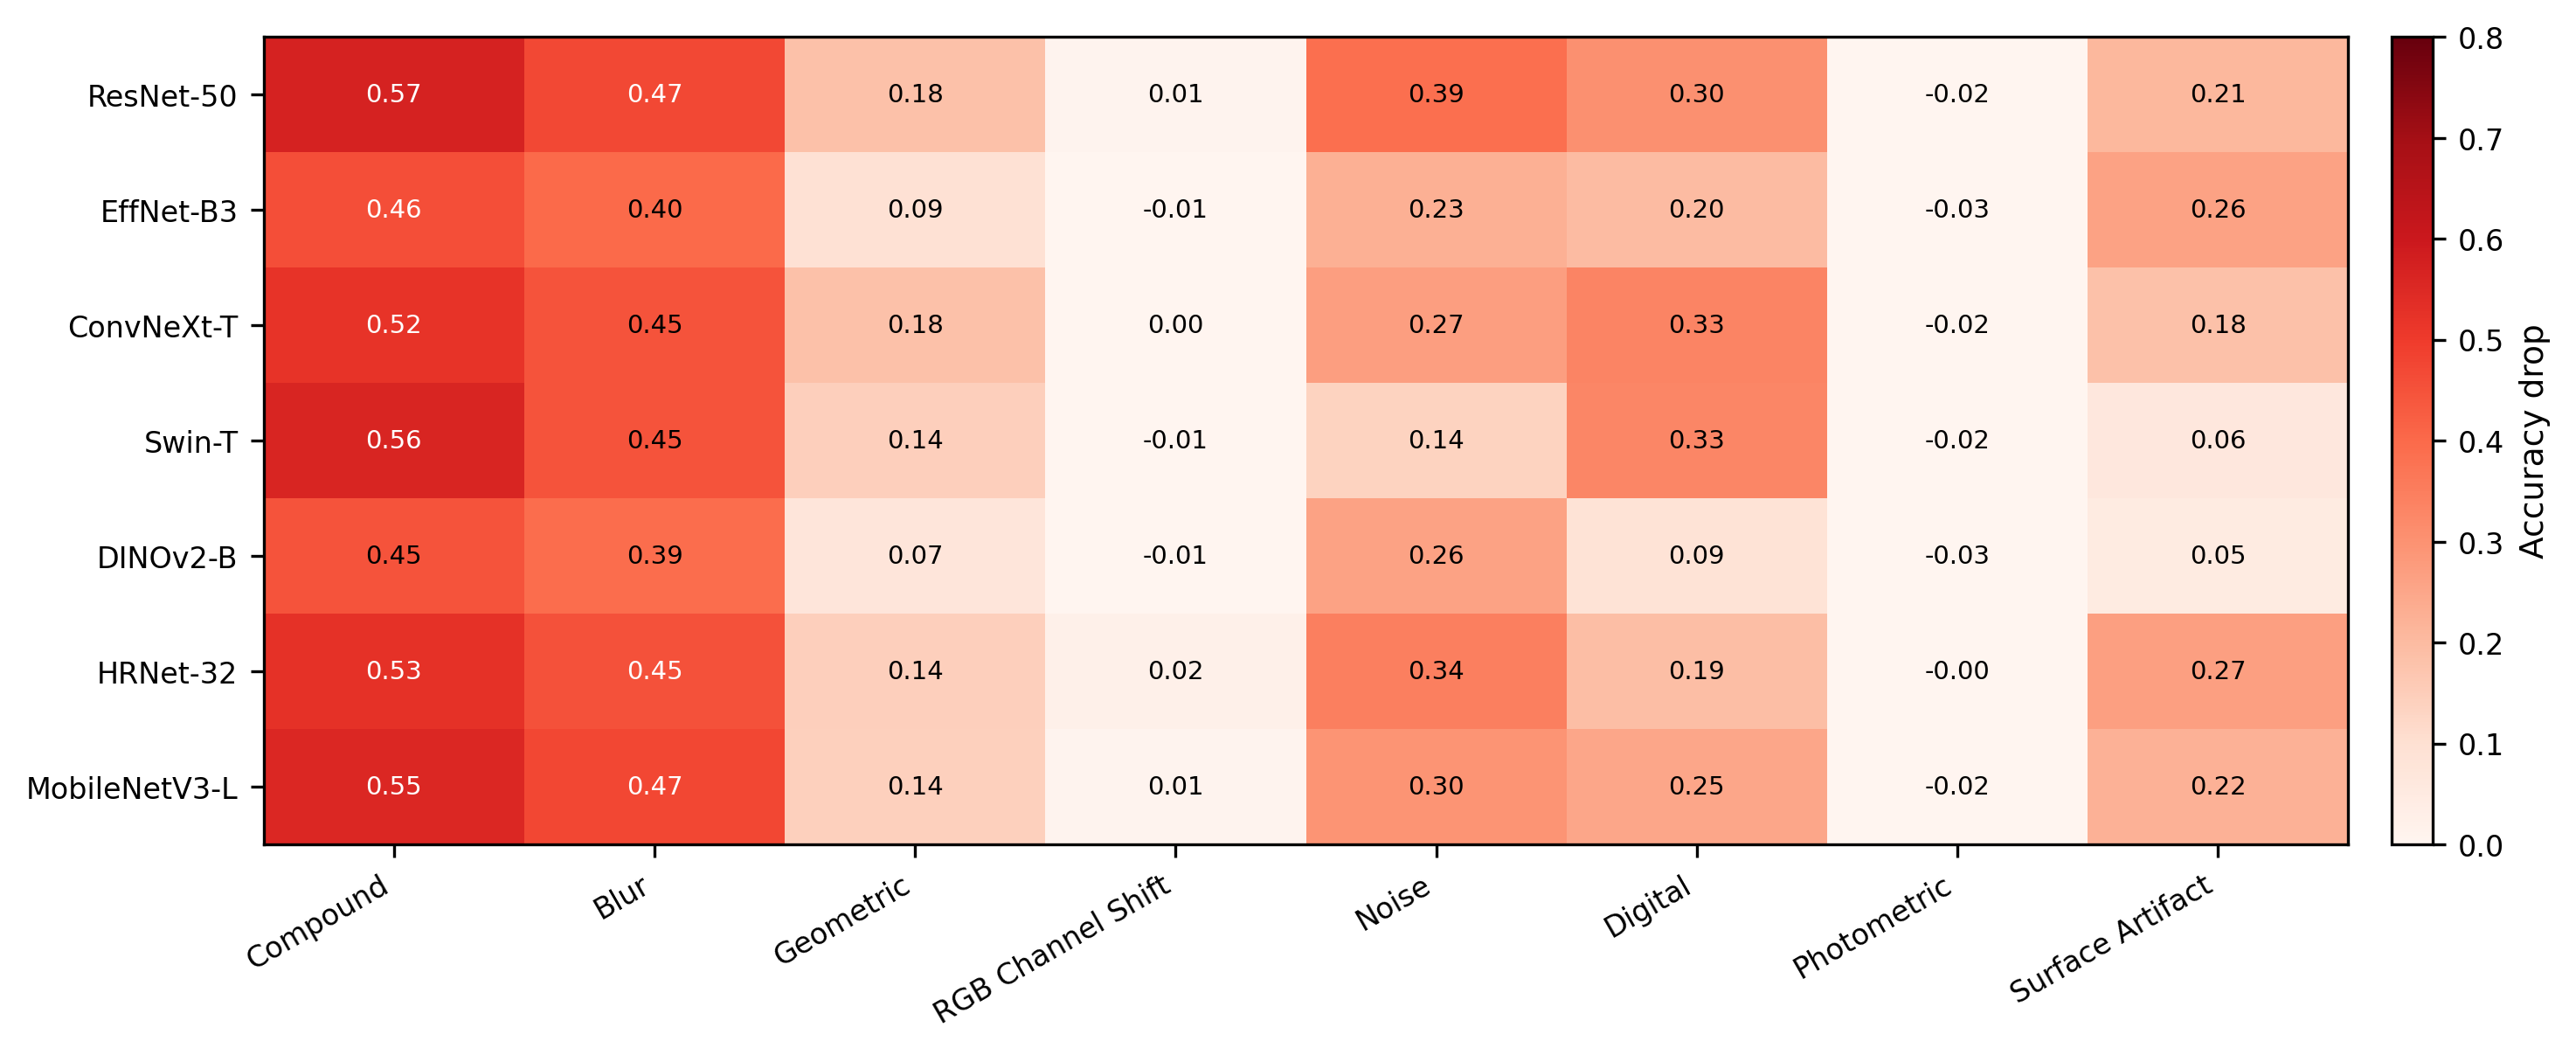
\includegraphics[width=\linewidth]{results/figures/fig2a_accuracy_heatmap.png}
\caption{Accuracy heatmap across backbones and perturbation families.}
\label{fig:acc_heatmap}
\end{figure}

\begin{figure}[pos=htbp]
\centering
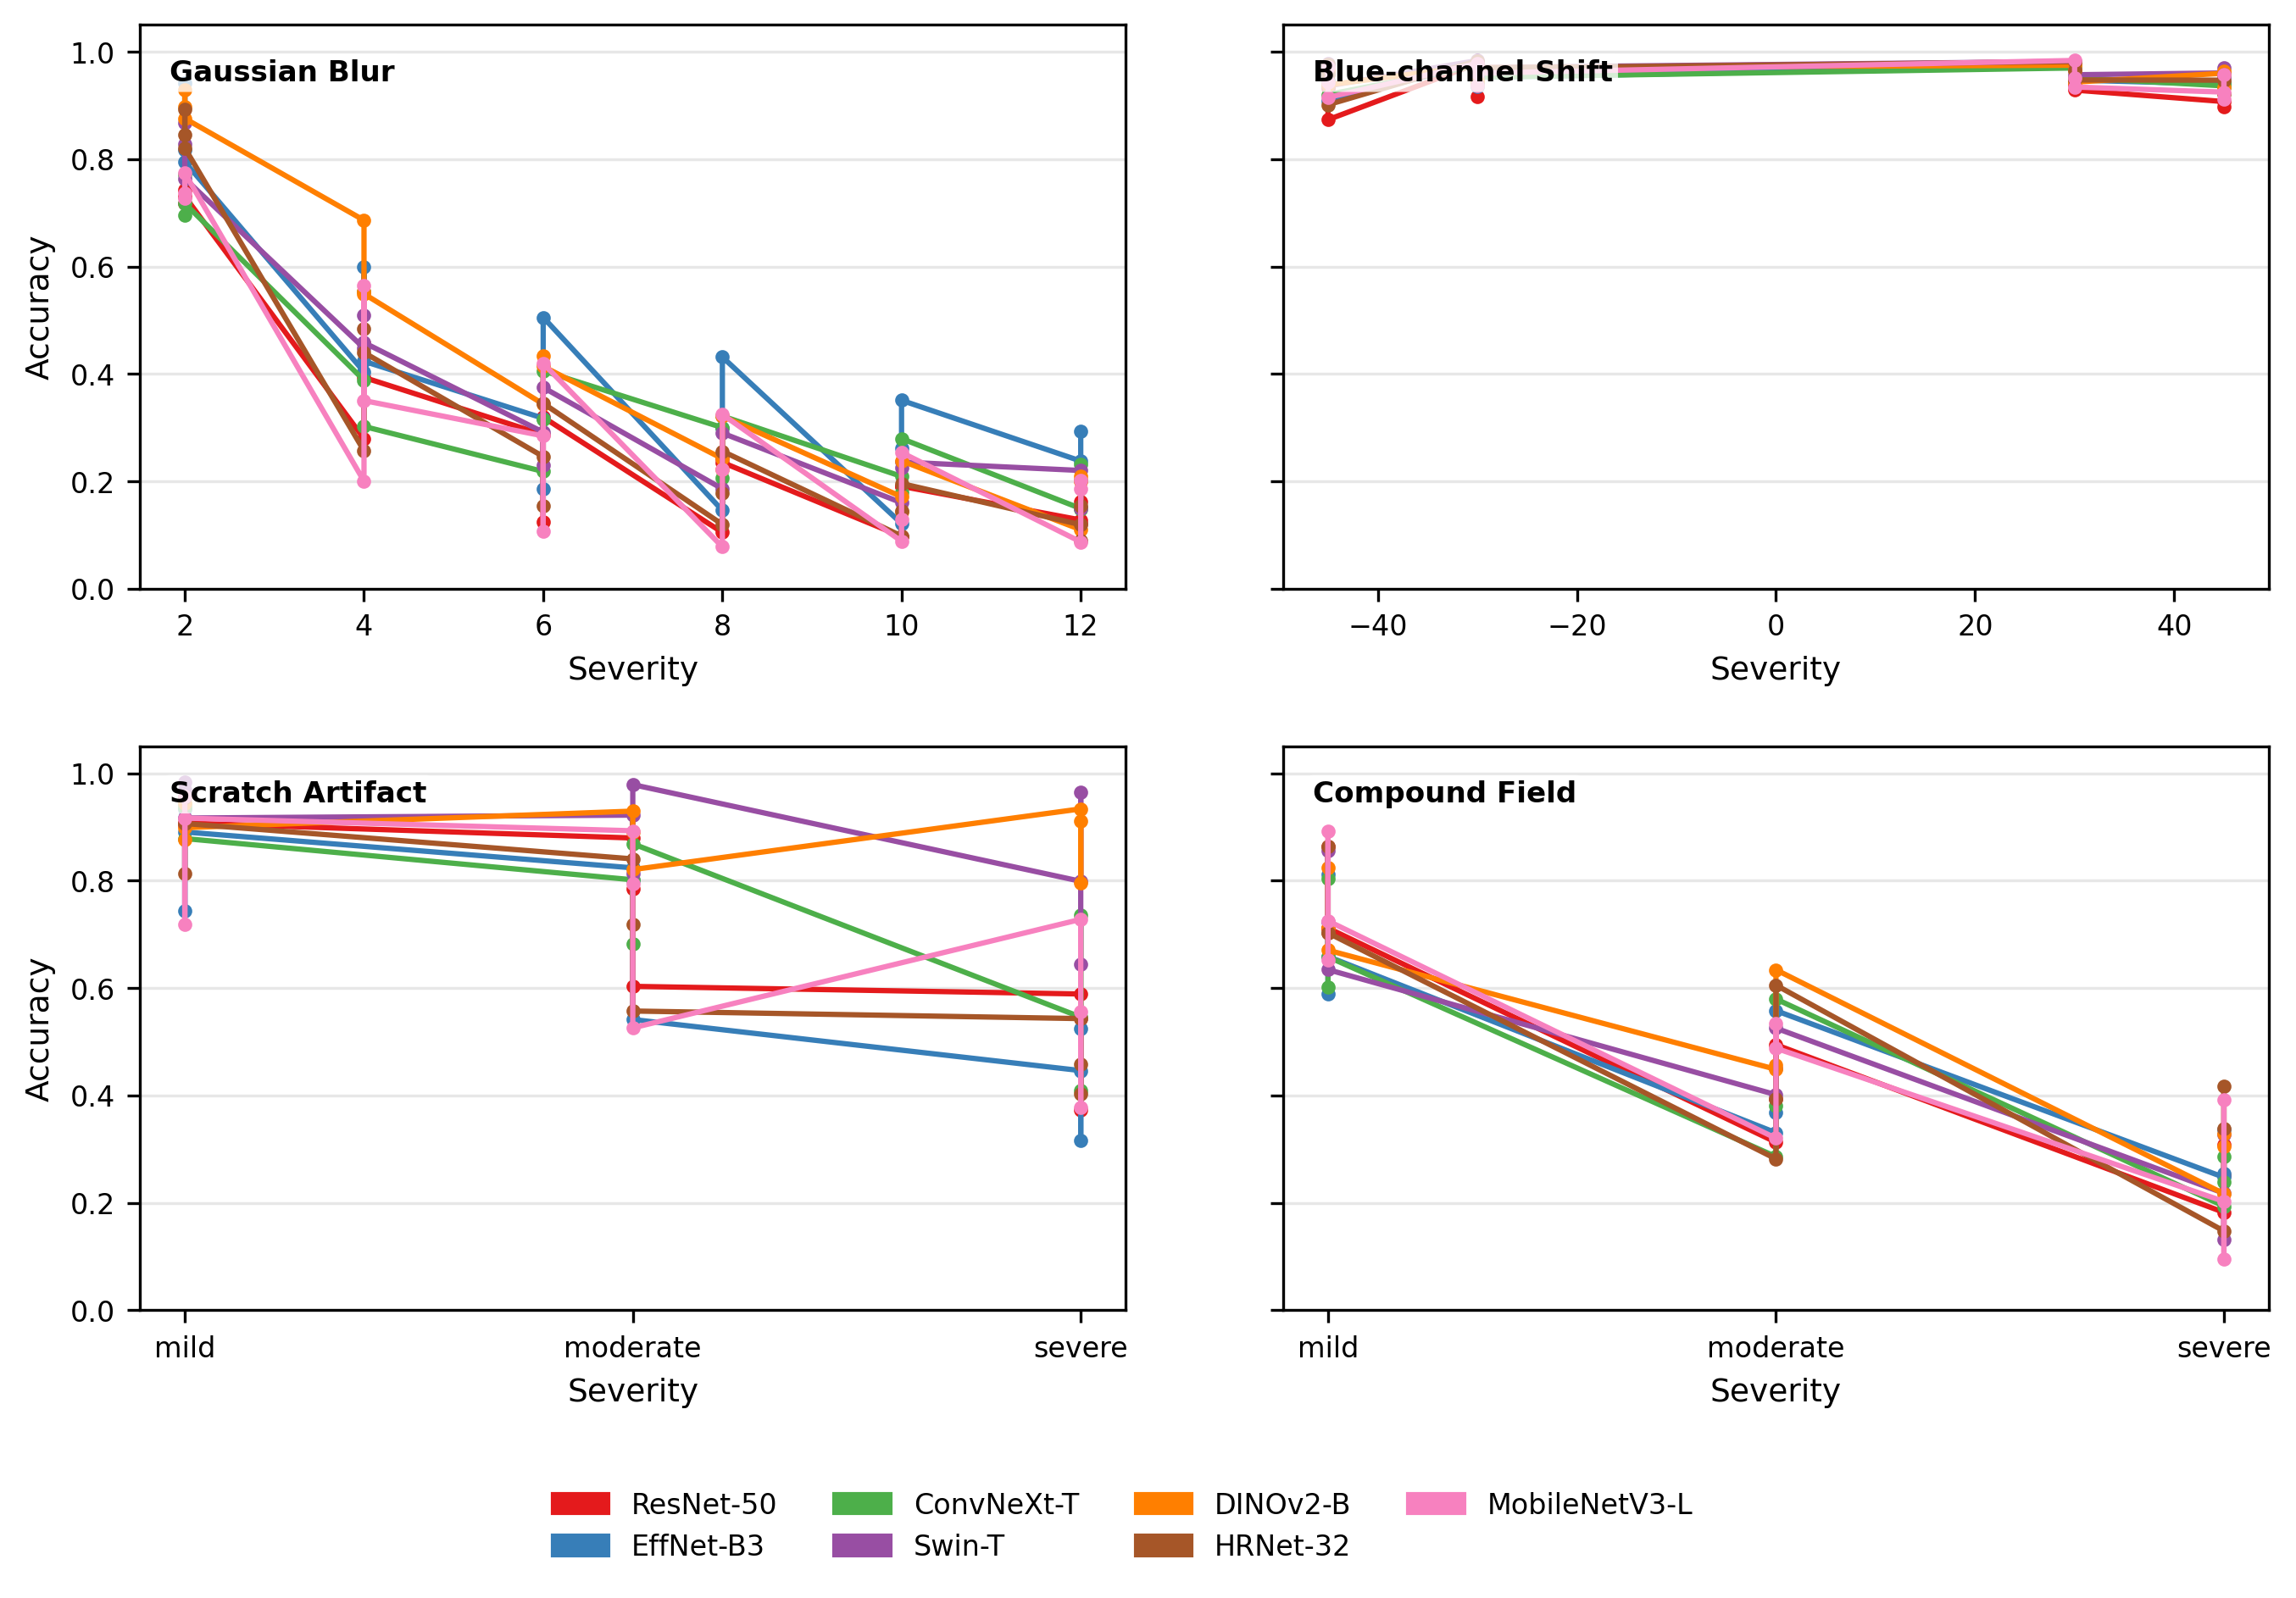
\includegraphics[width=\linewidth]{results/figures/fig2b_severity_curves.png}
\caption{Severity-dependent degradation curves with uncertainty estimates.}
\label{fig:severity}
\end{figure}

\begin{table}[pos=htbp]
\centering
\caption{Backbone robustness under synthetic perturbations.}
\label{tab:robustness}
\begin{tabular}{lccc}
\toprule
Backbone & Clean acc. & Perturbed acc. & Mean drop \\
\midrule
DINOv2-B & 0.938 & 0.736 & 0.203 \\
EfficientNet-B3 & 0.931 & 0.708 & 0.224 \\
Swin-T & 0.951 & 0.699 & 0.252 \\
HRNet-32 & 0.956 & 0.684 & 0.273 \\
ConvNeXt-T & 0.939 & 0.667 & 0.272 \\
MobileNetV3 & 0.942 & 0.665 & 0.276 \\
ResNet-50 & 0.935 & 0.638 & 0.297 \\
\bottomrule
\end{tabular}
\end{table}

Table~\ref{tab:perturbation} shows the perturbation hierarchy. Compound perturbations and blur-like degradations are most destructive, whereas the evaluated RGB channel shifts and global photometric changes do not consistently reduce accuracy in the averaged Tier-A setting. This is not a direct test of prior blue-channel findings \citep{owens2025robustness}, because the model, datasets, decision rule, and transform definitions differ. The safer conclusion is that perturbation ranking is parameter- and architecture-dependent, and that a broad stress-test suite exposes failure modes missed by narrower perturbation sets.

\begin{table}[pos=htbp]
\centering
\caption{Selected perturbation types ordered by mean accuracy drop.}
\label{tab:perturbation}
\begin{tabular}{lcc}
\toprule
Perturbation & Mean accuracy & Mean drop \\
\midrule
Compound & 0.219 & 0.723 \\
Gaussian blur & 0.357 & 0.585 \\
Compound optical & 0.448 & 0.494 \\
Pixelate & 0.460 & 0.482 \\
Compound field & 0.477 & 0.465 \\
Defocus blur & 0.494 & 0.448 \\
Shot noise & 0.553 & 0.389 \\
Zoom blur & 0.565 & 0.377 \\
Scratch & 0.762 & 0.180 \\
Resize & 0.832 & 0.110 \\
Blue-channel shift & 0.951 & -0.009 \\
\bottomrule
\end{tabular}
\end{table}

The statistical ranking analysis confirms that robustness ranking is not identical to clean-accuracy ranking. Across 228 non-clean dataset--perturbation--severity conditions, the Friedman test rejects equal backbone ranks ($\chi^2=243.945$, $p=8.06\times 10^{-50}$), with modest but non-negligible concordance (Kendall's $W=0.179$). The Nemenyi critical-difference analysis in Fig.~\ref{fig:nemenyi} gives the best mean ranks to DINOv2-B (2.882), Swin-T (3.145), and EfficientNet-B3 (3.601), while ResNet-50 has the weakest mean rank (5.469). In this diagram, lower mean rank means greater robustness, and backbones joined by a horizontal bar are not significantly different under the post-hoc rank comparison. The result shows that failure depends on the acquisition stressor and can reorder model preference, motivating the next question: which representation-level changes track the severity of these failures?

\begin{figure}[pos=htbp]
\centering
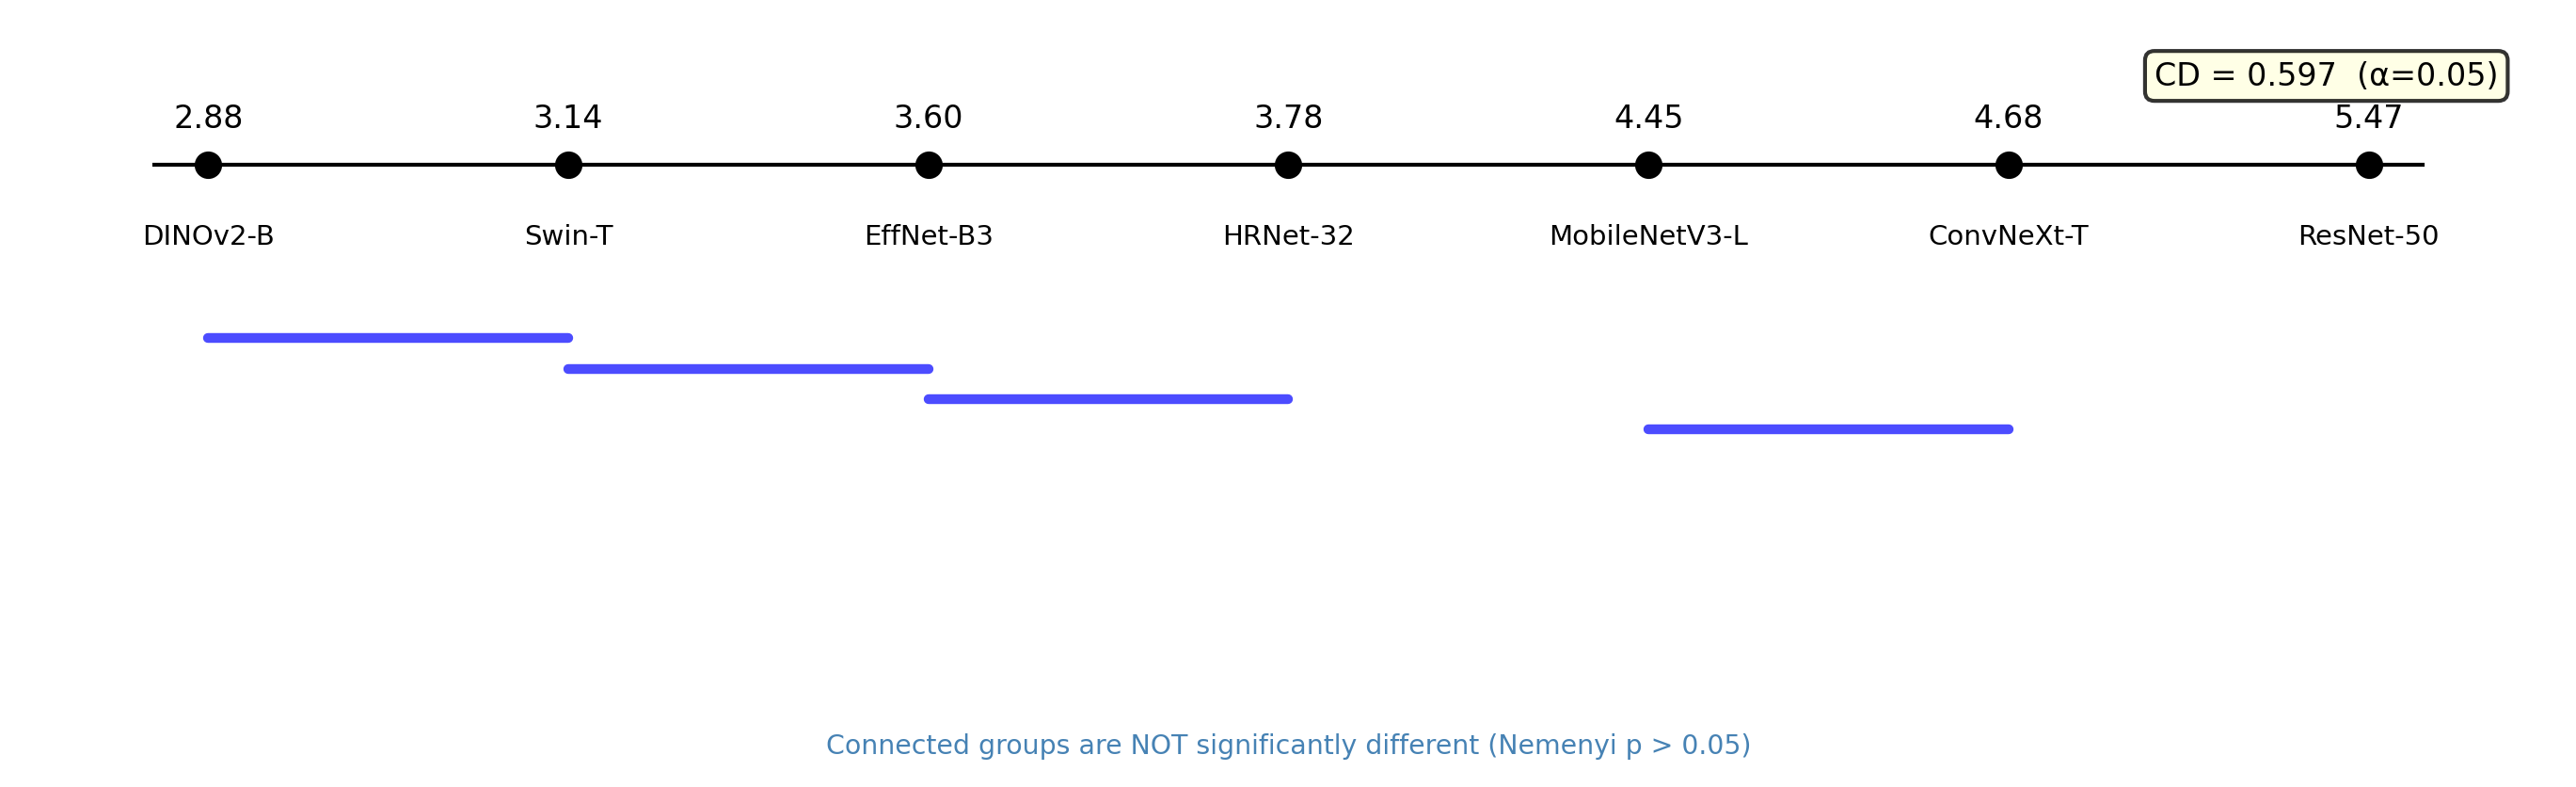
\includegraphics[width=.82\linewidth]{results/figures/fig5_nemenyi_cd_diagram.png}
\caption{Nemenyi critical-difference diagram for backbone robustness ranks over non-clean Tier-A conditions. Lower mean rank indicates stronger robustness.}
\label{fig:nemenyi}
\end{figure}

\subsection{Feature-space drift tracks accuracy degradation}
\label{sec:results_drift}

The robustness experiment shows where models fail; the feature-geometry experiment tests which representation-level changes track that failure. For each clean-shifted pair, we measure how far the shifted embedding moves from its clean counterpart and how the class geometry changes. If feature drift is only a trivial consequence of image perturbation, it should not strongly track the magnitude of accuracy degradation across different datasets, backbones, and perturbations. Conversely, if representation displacement is empirically linked to failure, larger drift should consistently correspond to larger accuracy drop.

Figure~\ref{fig:feature_geometry} and Table~\ref{tab:geometry_corr} support the latter interpretation. Feature drift has the strongest association with accuracy drop ($r=0.908$, $n=1596$, $p<10^{-300}$, i.e.\ below the double-precision floor). Inter-class collapse is also strongly related to degradation ($r=0.713$), indicating that shifted features reduce class separability. FGCS change has a weaker but still positive association ($r=0.340$), suggesting that the ratio between inter-class separation and intra-class compactness captures part of the failure but is less direct than paired feature displacement.

\begin{figure}[pos=htbp]
\centering
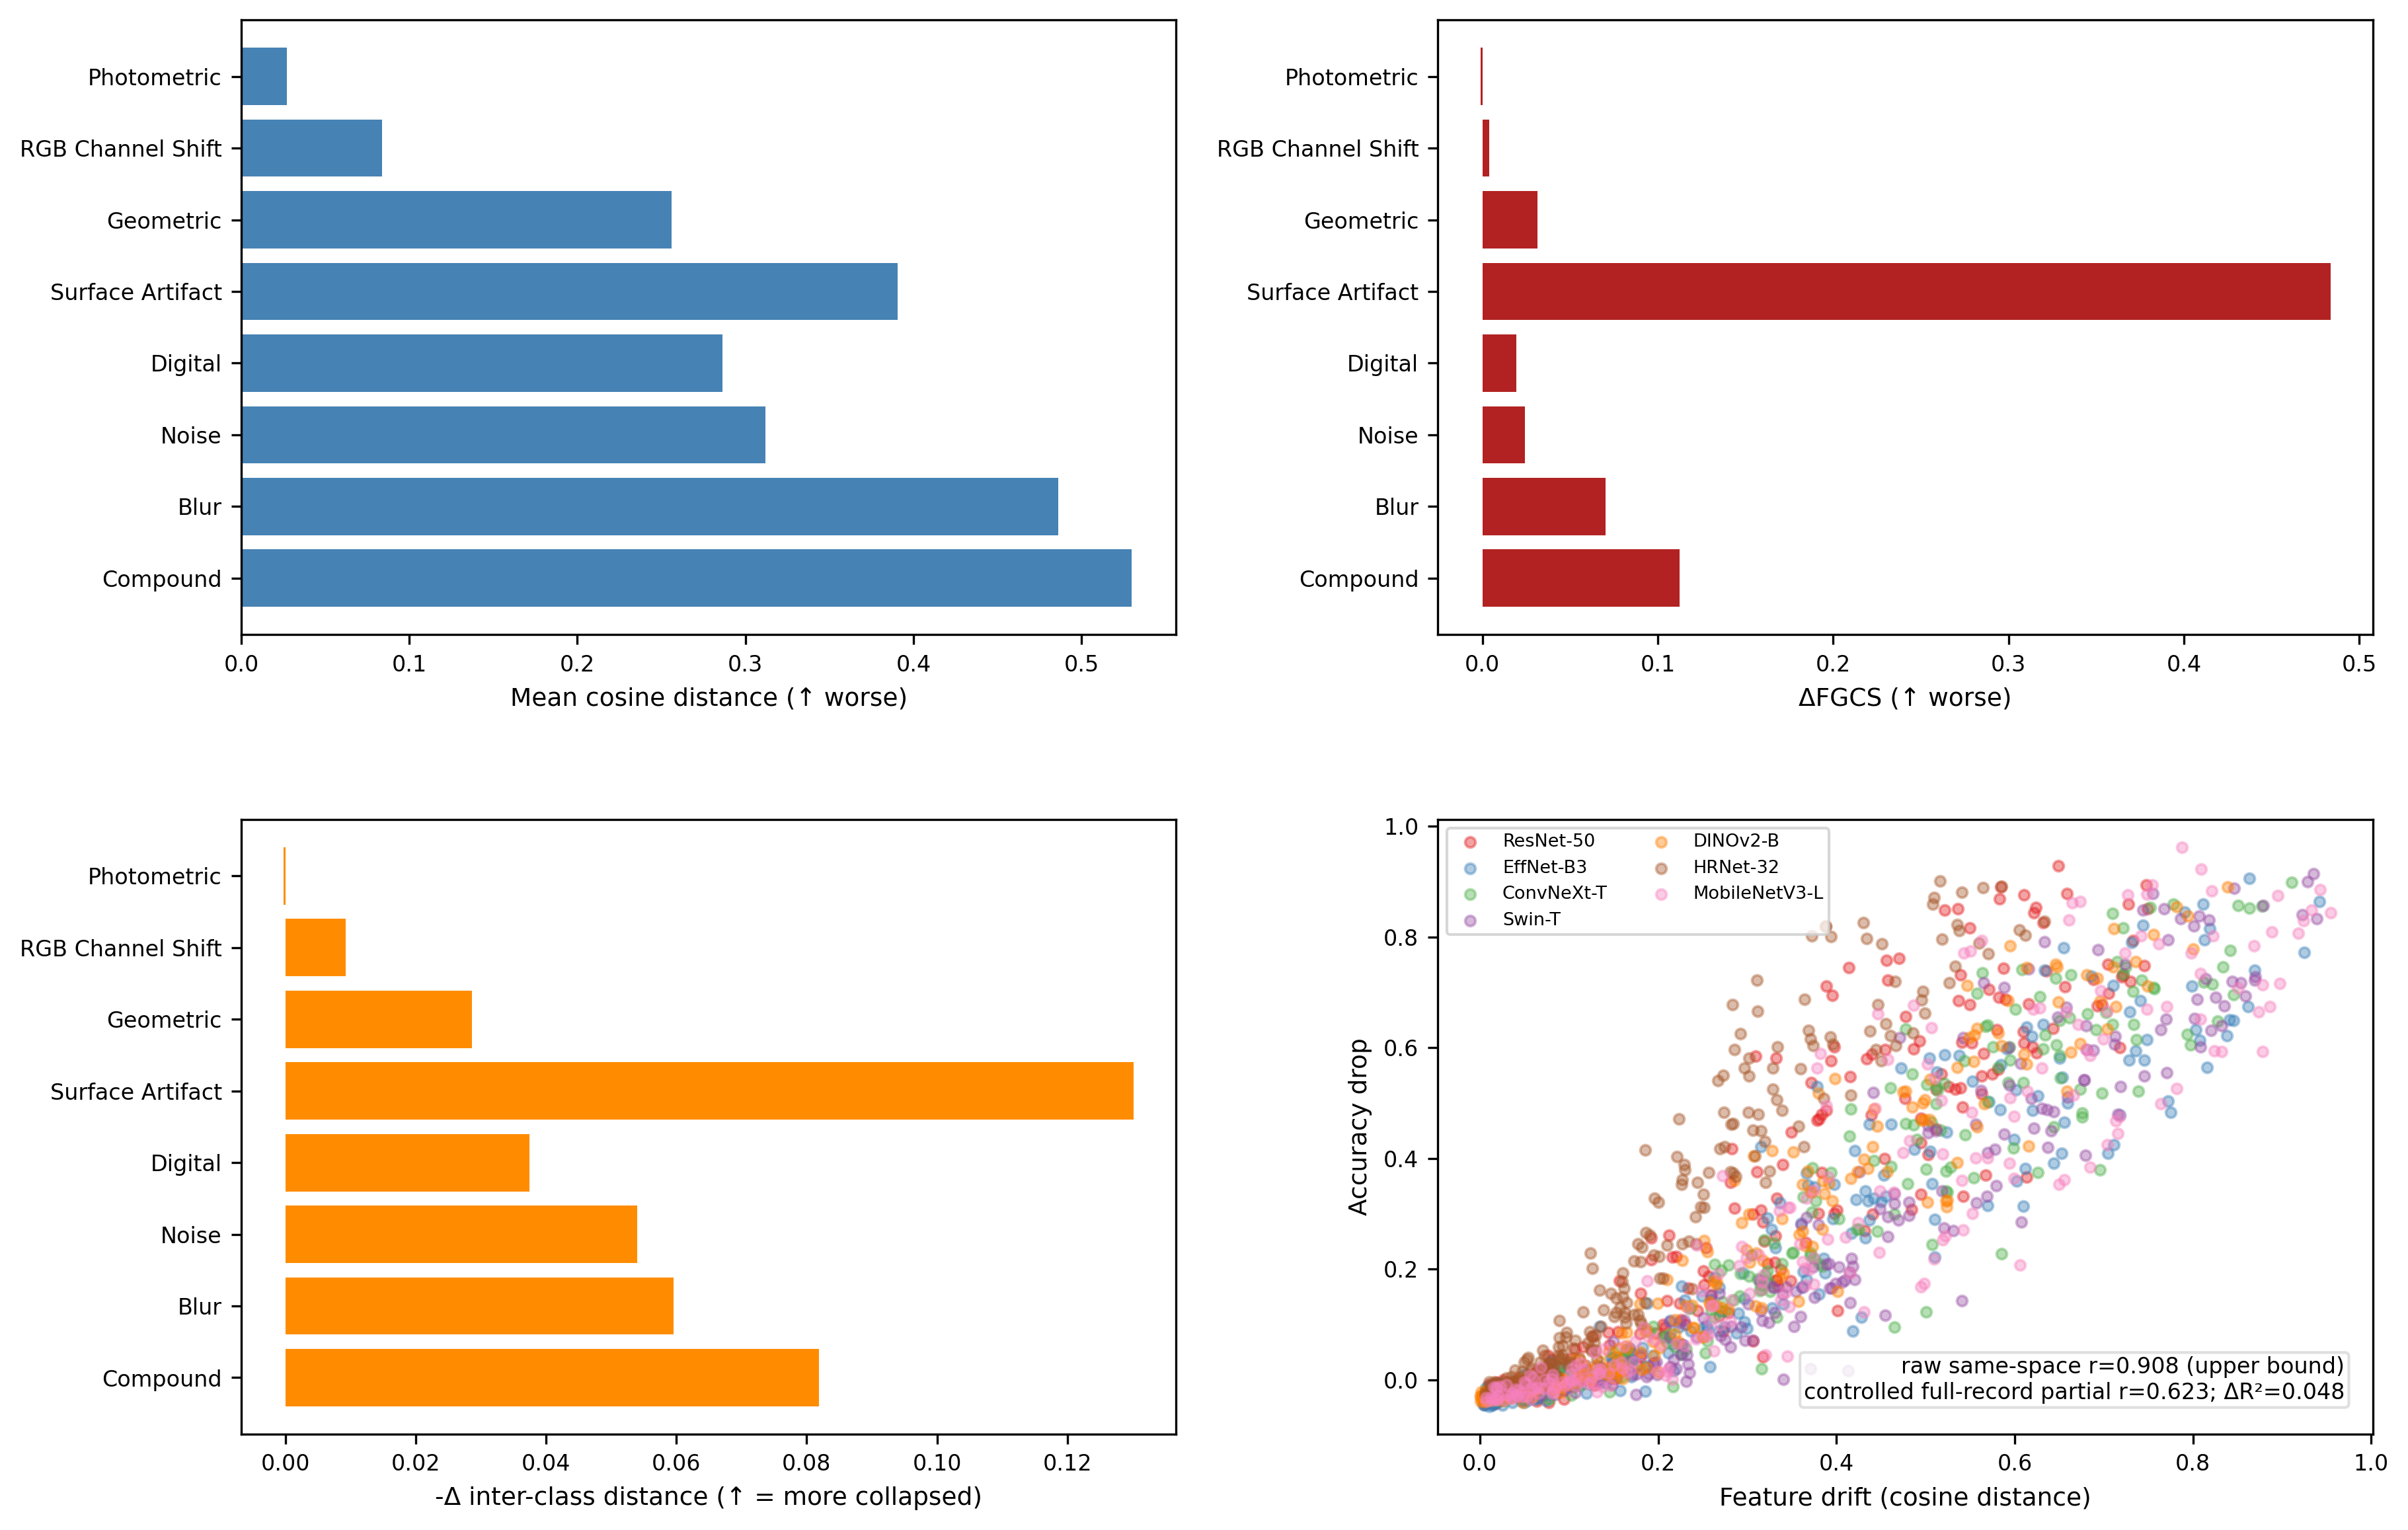
\includegraphics[width=\linewidth]{results/figures/fig3_feature_geometry_failure.png}
\caption{Feature geometry under acquisition shift. Feature drift is the strongest predictor of accuracy drop.}
\label{fig:feature_geometry}
\end{figure}

\begin{table}[pos=htbp]
\centering
\caption{Correlation between representation-geometry metrics and accuracy drop.}
\label{tab:geometry_corr}
\begin{tabular}{lcc}
\toprule
Metric & Pearson $r$ & $n$ \\
\midrule
Feature drift & 0.908 & 1596 \\
Inter-class collapse & 0.713 & 1596 \\
Intra-class change & -0.653 & 1596 \\
FSR collapse & 0.420 & 1596 \\
FGCS change & 0.340 & 1596 \\
\bottomrule
\end{tabular}
\end{table}

The conclusion is not based only on a pooled Pearson coefficient. Rank correlation gives the same ordering: feature drift has Spearman $\rho=0.937$ over the same 1596 records. After controlling for dataset, backbone, and perturbation family by residualization, the partial correlation between feature drift and accuracy drop remains high ($r=0.795$). The relationship is also consistent within every Tier-A dataset and every backbone, as summarized in Table~\ref{tab:consistency}. Leave-one-dataset-out validation remains strong: when each Tier-A dataset is held out in turn, the mean held-out feature-drift/drop correlation is $r=0.913$, with a minimum of $0.895$.

We test the margin mechanism of Section~\ref{sec:analytical} directly at the
sample level, using the prototype (nearest-centroid) rule for which
Proposition~1 is exact. Across 9,551,148 clean-correct sample--perturbation
records, 3,287,059 shifted samples flip under the prototype rule (34.4\%). For
each record we compute the clean margin $\Gamma(x)$ from Eq.~\eqref{eq:margin},
the paired drift $\Delta_f(x)$, and the margin gate $\Gamma(x)^2/8$. The
necessary condition of Corollary~\ref{eq:necessary} holds for 100.0\% of flipped
samples: no prototype flip occurs inside the provably safe region
$\Delta_f<\Gamma(x)^2/8$. The bound is deliberately worst-case and therefore
loose: it certifies only 0.3\% of records as guaranteed-correct, with a 0.0\%
flip rate inside that certified region. This explains why the right panel of
Fig.~\ref{fig:margin_crossing} is concentrated near small gates, while the left
panel shows the empirical effect that matters for prediction: flip rate rises
smoothly with total drift.

We then test whether direction-aware margin erosion in Eq.~\eqref{eq:firstorder}
materially improves per-sample flip prediction. Under the pooled Tier-A
sample-level evaluation, the clean-competitor shifted margin gives ROC-AUC 0.847,
only slightly above raw drift magnitude at 0.842 (gain 0.005), and the
single-competitor margin already drives a majority of failures: the region
$\widehat{\Gamma}(\hat z')\le 0$ is an exact sufficient condition for a flip and
captures 53.3\% of all flips with zero false positives (the vertical segment at
$\mathrm{FPR}=0$ in Fig.~\ref{fig:margin_direction}); the remaining 46.7\%
require a different margin-crossing route, such as a third class overtaking the
true class without the clean nearest-competitor condition being triggered. The
direction-aware signal is therefore consistent with the margin
mechanism but does not become the headline predictor under the pooled protocol.
The value of the analysis is mechanistic rather than a large predictive
improvement: drift tracks failure because it is the displacement term in a
margin-crossing condition that is never violated, while the worst-case
certificate is conservative because most feature movement is not aligned with the
clean margin direction.
Figure~\ref{fig:margin_direction} shows the corresponding ROC comparison.

\begin{figure}[pos=htbp]
\centering
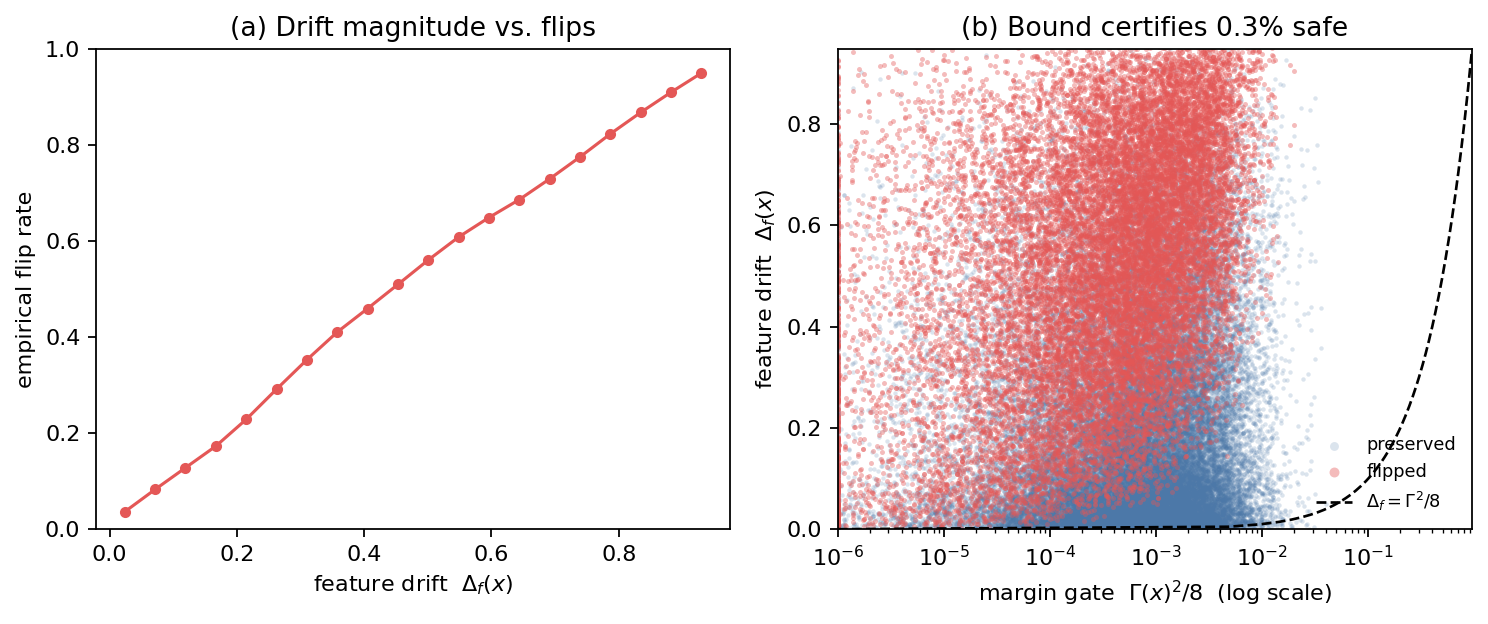
\includegraphics[width=.82\linewidth]{results/figures/fig_margin_crossing.png}
\caption{Margin-crossing validation of Proposition~1. Left: the empirical
prototype flip rate rises monotonically with paired feature drift. Right: the
worst-case margin gate $\Delta_f=\Gamma^2/8$ is never violated by flipped samples
but certifies only 0.3\% of records as guaranteed-correct, showing that the bound
is valid but conservative rather than a tight per-sample predictor.}
\label{fig:margin_crossing}
\end{figure}

\begin{figure}[pos=htbp]
\centering
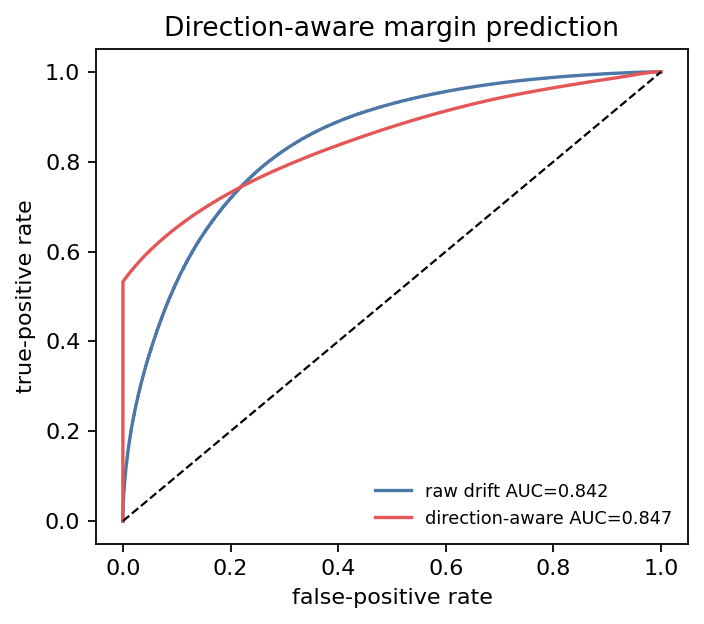
\includegraphics[width=.58\linewidth]{results/figures/fig_margin_direction.png}
\caption{Direction-aware margin check. The pooled flip ROC-AUC of
$\widehat{\Gamma}(\hat z')$ matches raw drift (0.847 versus 0.842), but the
operating point $\widehat{\Gamma}(\hat z')\le 0$ is an exact sufficient condition
for misclassification: it identifies 53.3\% of flips with zero false positives
(vertical segment), confirming that a majority of failures are deterministic
margin-crossing events against the clean nearest competitor.}
\label{fig:margin_direction}
\end{figure}

Whereas $\widehat{\Gamma}(\hat z')\le 0$ certifies the 53.3\% of flips in which
the clean nearest competitor overtakes the true class, that competitor is the
\emph{final} winner in only 26.2\% of all flips; in the remaining certified
cases a third class ultimately overtakes it. We therefore examine which class
becomes the final winner after a flip. Across 3,287,057 prototype flips, the
final winner is the clean nearest competitor in 26.2\% of cases. The remaining
73.8\% are competitor-switching failures in which a different class wins, but
they are still structured: among switched flips,
39.2\% of winners were already within the clean top-5 classes of the sample, and
the median clean rank is 7. This indicates a mixture of local confusions and
broader representation reordering rather than uniformly random labels. The
single-competitor share also varies strongly by stressor
(Fig.~\ref{fig:competitor_switching}b): illumination (82.2\%), blue-channel
shift (78.8\%), contrast (73.2\%), and red/green-channel shifts (71.8\%/69.1\%)
are mostly deterministic low-rank crossings, whereas compound degradation
(9.9\%), Gaussian blur (14.9\%), compound optical degradation (17.7\%), and
pixelation (18.8\%) induce broader multi-competitor switching. This extends the
margin account beyond the certified operating point: severe structure-destroying
stressors do not merely push the sample across one clean boundary, but can
reorder several nearby class margins at once.

\begin{figure}[pos=htbp]
\centering
\IfFileExists{results/figures/fig_competitor_switching.png}{%
  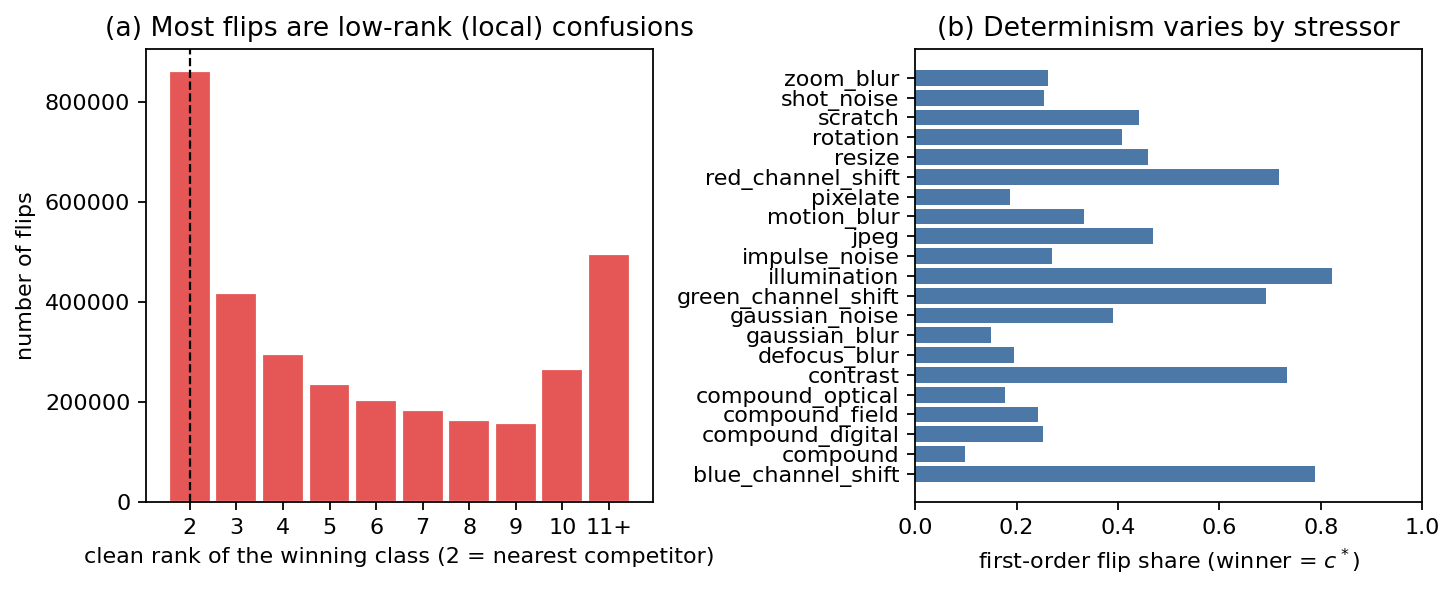
\includegraphics[width=\linewidth]{results/figures/fig_competitor_switching.png}%
}{%
  \fbox{\parbox{0.9\linewidth}{\centering Figure file missing: results/figures/fig\_competitor\_switching.png}}%
}
\caption{Structure of flips. (a) Clean rank of the winning class for flipped
samples (rank 2 = clean nearest competitor, deterministically certified by
$\widehat{\Gamma}(\hat z')\le0$ when it overtakes the true class). A majority of
flips have a low clean rank, but the long tail shows that severe shifts can
reorder several competitors. (b) Nearest-competitor (single-competitor)
winner share by perturbation family; photometric/channel shifts are more single-competitor, while blur,
pixelation, and compound degradation produce broader competitor switching.}
\label{fig:competitor_switching}
\end{figure}

Mixed-effects models further address grouped dependence. A random-slope model by backbone estimates a positive feature-drift effect ($\beta=1.155$, 95\% CI $[0.976,1.334]$, $p<0.001$). A crossed model with dataset and backbone effects, while controlling perturbation family and severity, still assigns feature drift a positive coefficient ($\beta=0.737$, 95\% CI $[0.692,0.783]$, $p<0.001$). A clustered bootstrap over dataset--backbone--perturbation groups gives $r=0.908$ with 95\% CI $[0.892,0.922]$. These checks reduce the risk that the main result is only a severity artifact, a single-dataset effect, or pseudo-replication.

\begin{table}[pos=htbp]
\centering
\caption{Consistency checks for the feature-drift/accuracy-drop relationship. Values are Pearson correlations computed within groups.}
\label{tab:consistency}
\footnotesize
\begin{tabular}{p{0.42\linewidth}p{0.25\linewidth}p{0.20\linewidth}}
\toprule
Grouping & Correlation range & Records per group \\
\midrule
Backbone & 0.926--0.965 & 228 \\
Tier-A dataset & 0.895--0.931 & 532 \\
Perturbation type & 0.594--0.902 & 63--126 \\
Leave-one-dataset-out & mean 0.913, min 0.895 & held-out datasets \\
Partial correlation with grouped controls & 0.795 & 1596 \\
Mixed model with grouped controls & $\beta=0.737$ & 1596 \\
\bottomrule
\end{tabular}
\end{table}

At the global representation level, failure is not merely a decision-layer artifact; it is accompanied by measurable feature displacement and class-geometry deformation. This also explains why feature drift later becomes a strong monitoring signal: it measures the same representation movement that tracks accuracy loss in the controlled experiments.

\subsection{Secondary spatial and CAM-proxy diagnostics}

Feature drift explains the magnitude of failure, but it does not by itself describe how the internal spatial organization changes across the wood surface. We therefore use spatial clustering and CAM-proxy redistribution as supporting diagnostics rather than as the primary predictive claim. Table~\ref{tab:spatial_cam_summary} summarizes the quantitative spatial and CAM-proxy metrics by backbone. Backbones differ in both spatial granularity and cluster stability: EfficientNet-B3 has the highest clean SGI (0.00950), whereas DINOv2-B and Swin-T have the highest Hungarian CSI (0.568 and 0.553). CAM-proxy redistribution also varies by architecture: DINOv2-B has the lowest CAM-JS distance (0.170), while ConvNeXt-T has the highest (0.363).

\begin{table}[pos=htbp]
\centering
\caption{Spatial and CAM-proxy diagnostic summary by backbone. SGI measures clean spatial granularity, CSI-H measures Hungarian-matched spatial cluster stability, and CAM-JS distance measures CAM-proxy cluster redistribution under shift.}
\label{tab:spatial_cam_summary}
\small
\begin{tabular}{lccc}
\toprule
Backbone & SGI $\uparrow$ & CSI-H $\uparrow$ & CAM-JS dist. $\downarrow$ \\
\midrule
EfficientNet-B3 & 0.00950 & 0.522 & 0.222 \\
MobileNetV3 & 0.00560 & 0.501 & 0.264 \\
HRNet-32 & 0.00494 & 0.480 & 0.228 \\
ResNet-50 & 0.00349 & 0.494 & 0.272 \\
DINOv2-B & 0.00174 & 0.568 & 0.170 \\
Swin-T & 0.00104 & 0.553 & 0.256 \\
ConvNeXt-T & 0.00065 & 0.476 & 0.363 \\
\bottomrule
\end{tabular}
\end{table}

\subsection{Cross-dataset and cross-magnification generalization}

The preceding experiments use controlled perturbations, which are necessary for paired drift analysis but may not fully represent public-dataset heterogeneity. We therefore use Tier-B datasets to test whether the feature-drift relationship survives external acquisition histories, and use VN26 cross-magnification transfer as a separate deployment-shift test focused on scale mismatch. Together, these experiments test whether the diagnostic relationship generalizes beyond Tier-A and whether deployment failure can also arise from scale mismatch rather than synthetic corruption alone.

The Tier-B validation in Fig.~\ref{fig:tierb} tests whether the feature-drift relationship holds outside the three Tier-A datasets. The correlation remains strong: Tier-A has $r=0.908$ with mean drop 0.257, while Tier-B has $r=0.870$ with mean drop 0.450. Because Tier-B datasets carry genuinely different acquisition histories rather than synthetic corruptions, the persistence of the drift/drop relationship there ($r=0.870$) is the strongest available evidence that the diagnostic is not an artefact of the synthetic protocol. Tier-B is also more difficult on average, as indicated by its higher mean drift and drop. This supports the claim that feature drift is not merely an artifact of the controlled Tier-A perturbation protocol.

These two settings are the closest available proxies for real deployment shift:
Tier-B datasets carry genuinely different acquisition pipelines (sensors,
capture conditions, and preparation) rather than synthetic corruptions, and
cross-magnification transfer on VN26 is a real optical scale change rather than
a simulated one. The persistence of the drift--drop relationship in both
settings is therefore the strongest available evidence that the diagnostic is
not an artefact of the synthetic perturbation protocol, in the absence of paired
laboratory-to-field captures.

\begin{figure}[pos=htbp]
\centering
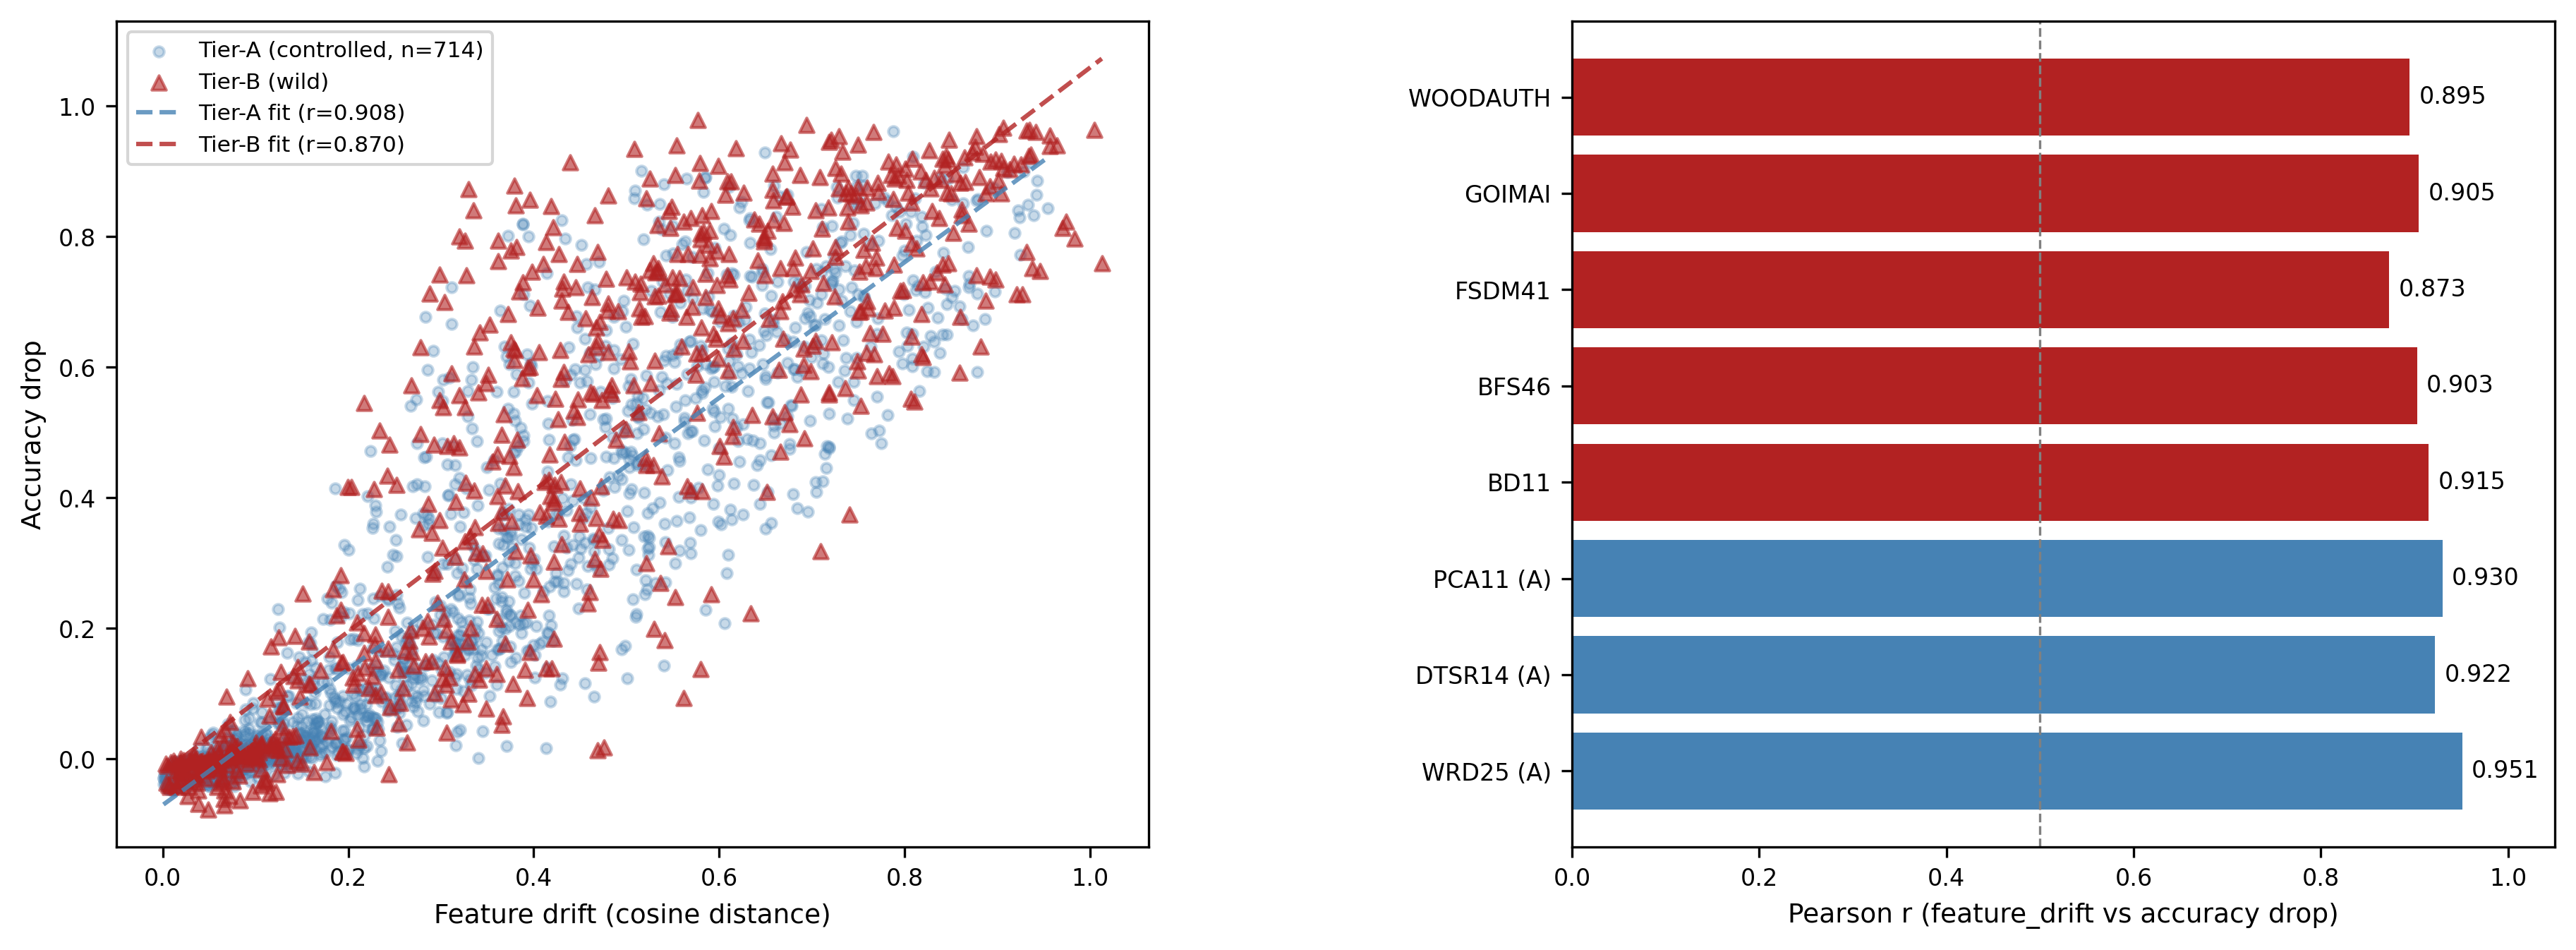
\includegraphics[width=\linewidth]{results/figures/fig11_tierb_validation.png}
\caption{Tier-B validation of the feature-drift relationship.}
\label{fig:tierb}
\end{figure}

Cross-magnification results on VN26 reveal this separate deployment scenario. Within-magnification accuracy is near perfect (0.996 at x10, 1.000 at x20, and 0.995 at x50). The full 3$\times$3 transfer matrix in Table~\ref{tab:crossmag} shows that accuracy drops sharply whenever the training and testing magnifications differ. Transfer from x10 to x20 remains partially viable (0.619), but transfer involving x50 is much weaker, especially x20$\rightarrow$x50 (0.160), x50$\rightarrow$x20 (0.179), and x10$\rightarrow$x50 (0.202). The transfer is also asymmetric: x10$\rightarrow$x20 (0.619) is markedly easier than x20$\rightarrow$x10 (0.537), and any transfer involving x50 collapses in both directions. This suggests that adapting from coarser to finer magnification is not symmetric to the reverse, consistent with anatomical detail being lost rather than recoverable across scale. The associated spatial stability analysis is shown in Appendix~\ref{app:spatial_cam}. These results indicate that magnification shift is not equivalent to ordinary synthetic perturbation: it changes the scale at which anatomical patterns are represented. Consequently, a WoodID system should not assume that robustness to blur or compression implies robustness to magnification changes, even when within-magnification recognition is almost saturated.

\begin{table}[pos=htbp]
\centering
\caption{VN26 full cross-magnification mean accuracy over seven frozen backbones. Diagonal entries are within-magnification baselines; off-diagonal entries use the source magnification as the clean gallery and the target magnification as the query set.}
\label{tab:crossmag}
\begin{tabular}{lccc}
\toprule
Train $\rightarrow$ Test & x10 & x20 & x50 \\
\midrule
x10 & 0.996 & 0.619 & 0.202 \\
x20 & 0.537 & 1.000 & 0.160 \\
x50 & 0.283 & 0.179 & 0.995 \\
\bottomrule
\end{tabular}
\end{table}

\subsection{Multilevel failure model}

The previous subsections analyze each signal separately. The multilevel model asks a stronger question: after accounting for perturbation type, which representation levels add independent explanatory value? This matters because a metric can correlate with failure simply because both are driven by perturbation severity. Hierarchical regression provides a structured way to separate the dominant effect of perturbation identity from the additional information carried by feature, spatial, and attention-level signals.

Table~\ref{tab:r2} shows that perturbation type alone explains $R^2=0.782$ of the accuracy drop in complete records with spatial and CAM-proxy measurements. Adding feature drift increases $R^2$ to 0.871, the largest incremental gain ($\Delta R^2=0.089$). Full feature geometry adds 0.017, spatial clustering adds 0.004, and attention drift adds 0.001. The ordering is consistent with the earlier analyses: global feature displacement is the main quantitative bridge between shift and failure, while spatial and CAM-proxy metrics provide smaller but interpretable refinements. Because this table is intended as an interpretable variance-partitioning analysis, Table~\ref{tab:hier_strict} reports a stricter complete-case model with dataset, backbone, perturbation family, and severity controls.

\begin{table}[pos=htbp]
\centering
\caption{Hierarchical regression for accuracy-drop explanation.}
\label{tab:r2}
\begin{tabular}{lcc}
\toprule
Model & $R^2$ & $\Delta R^2$ \\
\midrule
Perturbation type only & 0.782 & 0.782 \\
+ Feature drift & 0.871 & 0.089 \\
+ Full feature geometry & 0.888 & 0.017 \\
+ Spatial clustering & 0.893 & 0.004 \\
+ Attention drift & 0.894 & 0.001 \\
\bottomrule
\end{tabular}
\end{table}

The multilevel model therefore provides the synthesis for the representation analysis: feature drift is the dominant explanatory level after accounting for perturbation identity, while class geometry, spatial clustering, and CAM-proxy redistribution add smaller interpretive information.

\subsection{Label-free deployment failure monitoring}
\label{sec:monitoring_results}

The final experiment converts the diagnostic findings into a deployment setting. Paired feature drift is powerful in controlled experiments, but it is not directly deployable because a field system does not observe both a clean and shifted version of the same image. We therefore construct a clean reference bank for each dataset/backbone and score shifted deployment batches without target labels. A record is counted as a recognition-failure case when its kNN accuracy drop exceeds 0.20, corresponding to a practically meaningful 20-percentage-point degradation that would normally justify reacquisition or manual review in a screening workflow. Labels are used only to define this retrospective evaluation target, not to compute the monitor score. This setting is closer to a real WoodID monitor: the system has access to validated reference features from its acquisition protocol and must decide whether an incoming batch has drifted enough to risk failure.

Table~\ref{tab:monitor} reports the detector results over 4256 backbone--dataset--perturbation records, with bootstrap confidence intervals for ROC-AUC and F1. The best deployable detector, RBF-MMD, reaches ROC-AUC 0.968 (95\% CI 0.964--0.973) and F1 0.909 (95\% CI 0.902--0.918), approaching the paired feature-drift oracle (ROC-AUC 0.976). Centroid cosine and kNN distances are also strong, with ROC-AUC values above 0.958 for the best two alternatives. Under this batch-level synthetic-shift benchmark, deployment failure can be detected without target labels and without clean-shifted pairs, provided that a representative clean reference bank is available.

Figure~\ref{fig:monitor_roc} complements this deployment result by showing the controlled diagnostic upper bound: the paired feature-drift oracle reaches ROC-AUC 0.975 and remains stable when the accuracy-drop threshold defining retrospective positives varies from 0.10 to 0.40 (ROC-AUC range 0.963--0.984). The AUC panel also shows a clear ordering among diagnostic signals: feature drift is strongest, class-geometry collapse is next, and spatial/CAM-proxy-derived signals remain useful but weaker. This ranking is consistent with the rest of the paper. Global feature displacement is the most compact predictor of failure magnitude, while spatial and CAM-proxy signals are better interpreted as secondary diagnostic evidence.

\begin{figure}[pos=htbp]
\centering
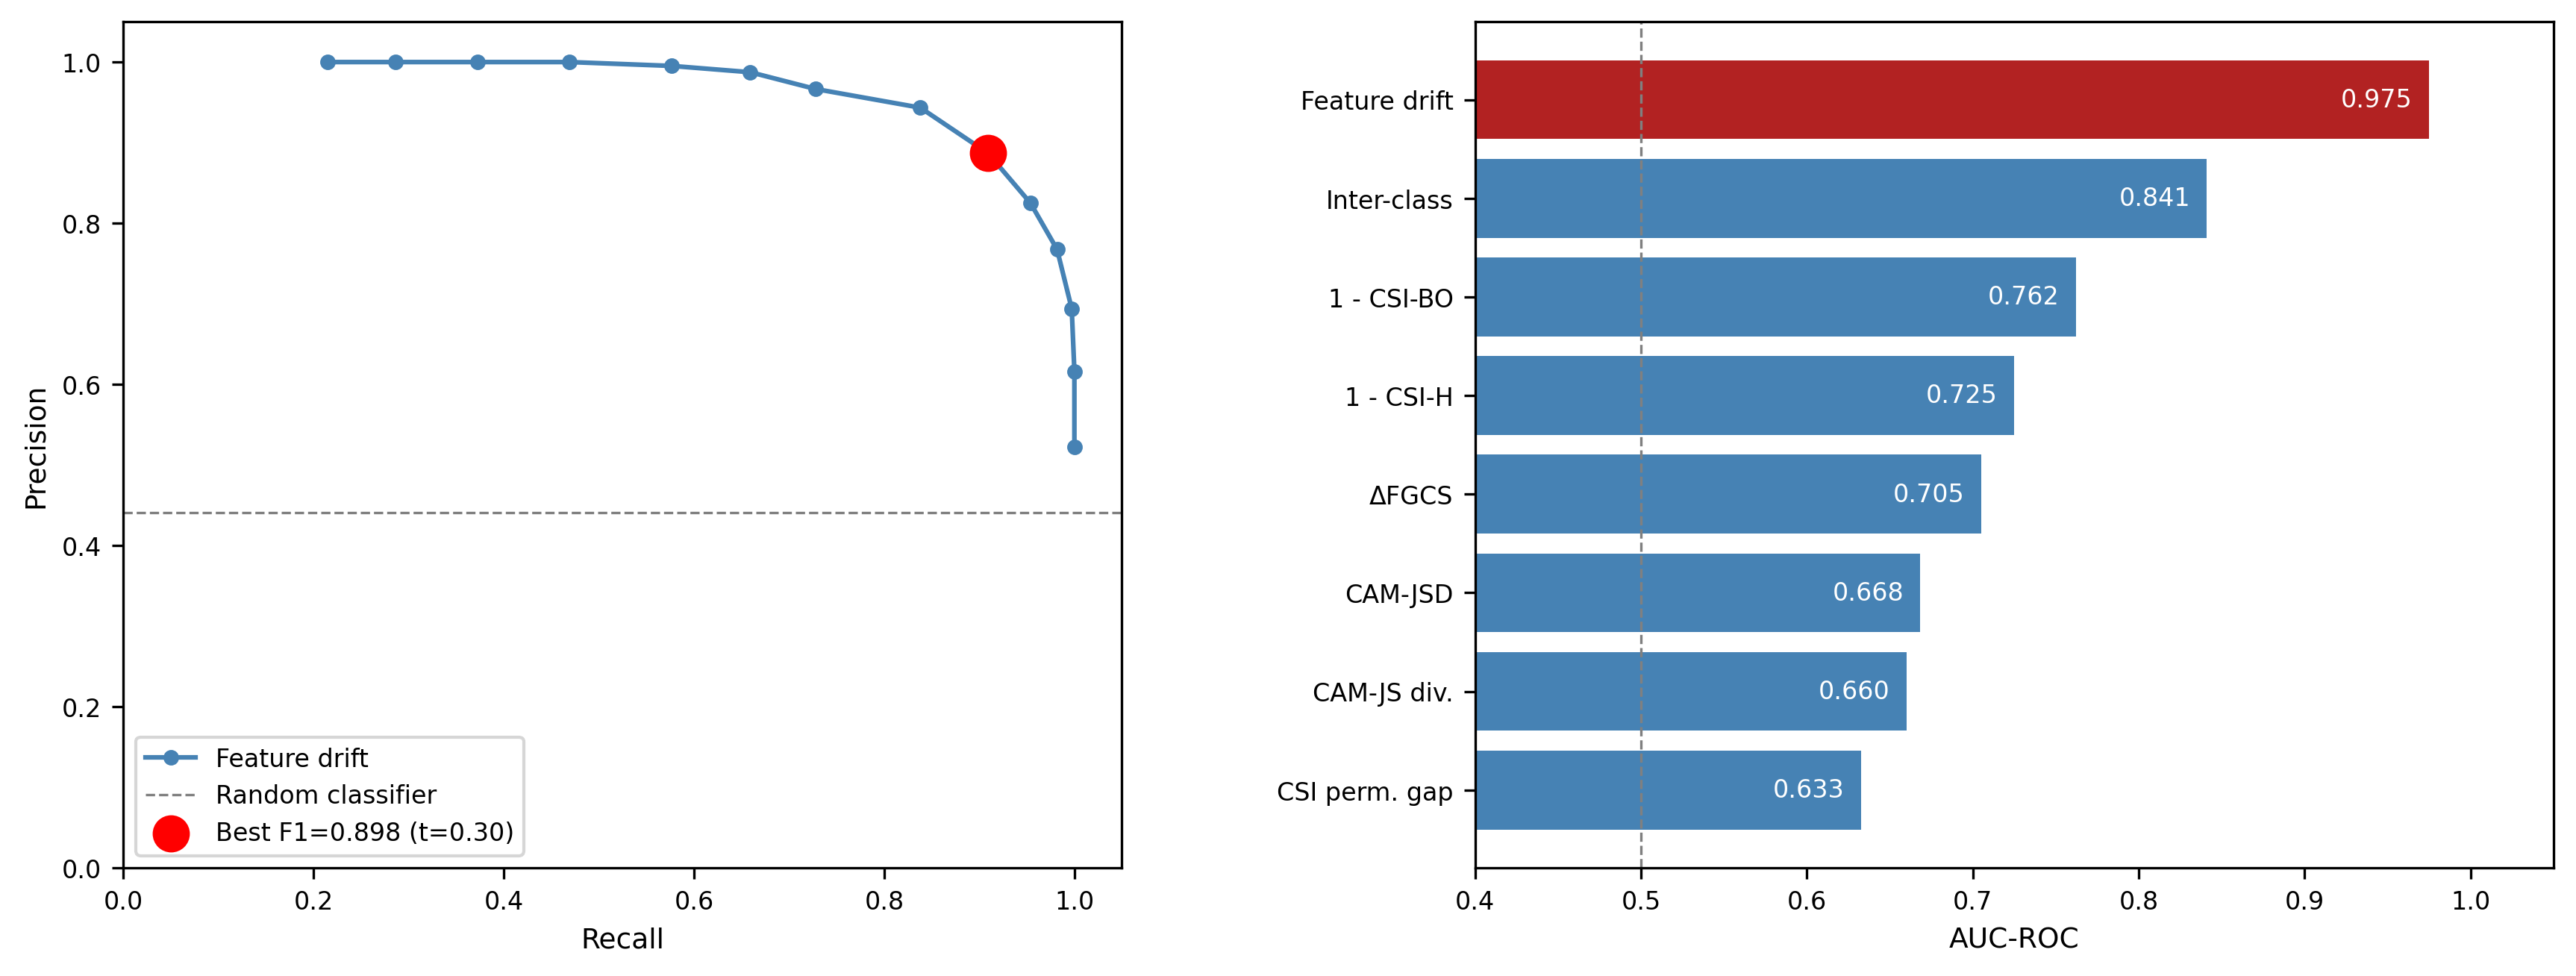
\includegraphics[width=\linewidth]{results/figures/fig8_roc_failure_detection.png}
\caption{Controlled diagnostic failure detection using representation-level signals. The paired feature-drift score is an oracle because it requires clean-shifted pairs; deployable reference-bank detectors are summarized separately in Table~\ref{tab:monitor}.}
\label{fig:monitor_roc}
\end{figure}

Additional checks make the monitor claim more deployment-oriented. With batch size 8, RBF-MMD ROC-AUC remains between 0.924 and 0.930 depending on reference-bank size; with batch sizes 32--64, ROC-AUC increases to roughly 0.961--0.977 (Table~\ref{tab:batch_ref}). Fixed-operating-point analysis shows that RBF-MMD recovers 81.0\% of failures at 5\% FPR and 90.8\% at 10\% FPR (Table~\ref{tab:mmd_oppoints}). Leave-one-dataset-out threshold transfer remains strong: when the threshold is calibrated on seven datasets and evaluated on the held-out dataset, RBF-MMD obtains mean ROC-AUC 0.974, minimum ROC-AUC 0.964, mean F1 0.895, and minimum F1 0.824 across the eight datasets. Leave-one-perturbation-family-out evaluation is harder: RBF-MMD obtains mean held-out ROC-AUC 0.946 and mean held-out F1 0.675, because a threshold selected on known families can be conservative for low-failure families such as channel shift and illumination (Table~\ref{tab:lopo}). Thus, reference-bank monitoring is a strong label-free risk signal, but threshold calibration remains a real deployment issue for unseen shift types.

\begin{table}[pos=htbp]
\centering
\caption{Reference-bank deployment failure detection. Brackets show 95\% bootstrap confidence intervals. The paired feature-drift detector is an oracle because it requires clean-shifted pairs; all reference-bank detectors are deployable.}
\label{tab:monitor}
\small
\begin{tabular}{lcccc}
\toprule
Detector & Deploy. & ROC-AUC & AP & Best F1 \\
\midrule
RBF-MMD & Yes & 0.968 [0.964, 0.973] & 0.967 & 0.909 [0.902, 0.918] \\
Centroid cosine & Yes & 0.959 [0.954, 0.964] & 0.958 & 0.897 [0.889, 0.907] \\
kNN-1 distance & Yes & 0.958 [0.953, 0.963] & 0.957 & 0.892 [0.884, 0.902] \\
kNN-5 distance & Yes & 0.942 [0.935, 0.948] & 0.945 & 0.872 [0.862, 0.883] \\
Mahalanobis delta & Yes & 0.916 [0.908, 0.924] & 0.911 & 0.850 [0.840, 0.861] \\
Mahalanobis & Yes & 0.915 [0.907, 0.923] & 0.911 & 0.851 [0.840, 0.861] \\
Paired feature drift & No & 0.976 [0.973, 0.979] & 0.977 & 0.919 [0.911, 0.928] \\
\bottomrule
\end{tabular}
\end{table}

The practical implication is that feature drift should be viewed in two forms. The paired version is a controlled upper-bound diagnostic for the representation-failure mechanism. The reference-bank version is the operational monitor: it compares incoming features to the clean reference bank $B_0$ and can trigger reacquisition, calibration, or manual review. The small gap between RBF-MMD and the oracle paired drift strengthens the central claim that representation drift is not only explanatory but also operationally useful in the evaluated setting. Because the monitoring benchmark uses synthetic batch-level shift, its absolute operating points should be read as an upper-bound estimate pending validation on real field batches. The sensitivity and held-out-family results also clarify the boundary of this deployment claim: the score transfers well as a ranking signal, but an operational alarm threshold should be calibrated for the expected batch size, reference-bank coverage, and acquisition condition.

\subsection{Negative control: restoration does not reduce drift}

A final negative-control experiment tests whether a visually plausible restoration step automatically reduces representation drift. On Gaussian-blur conditions, Wiener deconvolution makes this assumption fail rather than succeed: averaged over 126 backbone--dataset--blur-radius records, blurred accuracy is 0.469, while deblurred accuracy drops to 0.297; mean paired drift increases from 0.488 to 0.638. Deblurring improves accuracy in only 10.3\% of records and reduces representation drift in only 8.7\% of records. The per-radius results are reported in Table~\ref{tab:deblur}. This result supports the deployment-monitoring argument: acquisition-quality corrections should be validated through representation stability and recognition behavior, rather than assumed to improve robustness because they make images look sharper.

\subsection{Augmentation reduces but does not remove the failure, and the diagnostic persists}
\label{sec:augmentation}

Because the perturbation suite is also an augmentation family, we test whether
training the decision head on clean plus perturbed features (input-augmentation
training under the frozen backbone) closes the gap. On DINOv2-B/WRD25 with a
linear ridge head, augmentation raises mean perturbed accuracy by 0.243 and
shrinks the clean-to-perturbed gap from 0.333 to 0.075
(Table~\ref{tab:augmentation}), but a residual gap remains and clean accuracy
drops slightly (0.968 to 0.953). Crucially, the drift--drop relationship
persists under the augmented head (Pearson $r=0.909$ versus 0.971 for the
baseline head), so representation drift remains a valid diagnostic even after
augmentation; augmentation mitigates the failure rather than eliminating the
need to monitor it.
This gain is, however, obtained for shift families that are known and simulated
in advance: the augmented head is trained and evaluated on the same perturbation
families. It therefore does not address unanticipated field shifts---exactly
where a label-free monitor is needed---consistent with the
leave-one-perturbation-family-out result (Table~\ref{tab:lopo}), where a
threshold calibrated on known families transfers only partially to held-out
ones.

\begin{table}[pos=htbp]
\centering
\caption{Frozen linear ridge head versus augmentation-trained linear ridge head (DINOv2-B/WRD25; frozen backbone). Augmentation reduces but does not remove the gap; the drift--drop relationship persists.}
\label{tab:augmentation}
\begin{tabular}{lcccc}
\toprule
Head & Clean acc. & Perturbed acc. & Gap & drift$\to$drop $r$ \\
\midrule
Baseline (clean only) & 0.968 & 0.635 & 0.333 & 0.971 \\
Augmented (clean+pert.) & 0.953 & 0.878 & 0.075 & 0.909 \\
\bottomrule
\end{tabular}
\end{table}

\FloatBarrier

\section{Discussion}

The experiments give a connected picture of WoodID failure under acquisition shift. Pretrained backbones do not fail in a single uniform way: clean accuracy, synthetic-shift robustness, and cross-magnification transfer can produce different model rankings. Among the measured representation-level signals, paired feature drift is the dominant quantitative marker of degradation, while class geometry, spatial clustering, and CAM-proxy redistribution provide secondary explanatory detail. The same principle can be operationalized without target labels through a clean reference bank $B_0$, although threshold calibration remains shift-family dependent. The discussion below synthesizes these findings rather than repeating each experiment.

\subsection{Feature drift is the dominant failure signal}

Across the experiments, feature drift is the most consistent signal of failure. It correlates strongly with accuracy drop, contributes the largest incremental $R^2$ beyond perturbation identity, generalizes from Tier-A to Tier-B, remains stable in leave-one-dataset-out validation, survives mixed-effects controls, and provides the bridge to deployment monitoring. The central reason is that the frozen-backbone kNN protocol makes representation geometry directly responsible for the prediction. If a shifted image remains close to its clean representation and to the same local class neighbourhood, the nearest-neighbour decision is more likely to remain stable. If the feature moves away from that neighbourhood, collapses toward other species regions, or becomes less class-separable relative to the clean reference bank $B_0$, errors become more likely. In this setting, feature drift is not merely a descriptive embedding statistic; it measures the same geometry that the classifier uses at inference time.

We address the most important objection to this result directly: because the decision rule is a cosine $k$NN in the same embedding space in which $\Delta_f$ is measured, one might expect feature drift and accuracy drop to be coupled by construction. This coupling is real but the relationship is not a tautology. Drift is a continuous cosine displacement, whereas an error is a thresholded label flip that depends on the local class density and margin around the clean feature: a sample can move substantially yet remain inside its own high-density class region without changing its nearest-neighbour vote, while a small displacement near a decision boundary can flip the label. The empirical content of our result is therefore not the existence of a correlation but its tightness and stability across heterogeneous datasets, backbones, and perturbation families, after residualizing the shared severity component (partial $r=0.795$), and the fact that the same displacement signal transfers to a label-free reference-bank monitor. To further separate the signal from one decision rule, Appendix~\ref{app:additional_checks} shows that the drift/drop association persists under nearest-centroid classification and under a frozen linear probe trained on clean training-split features and evaluated on perturbed test-split features. This argument is made precise in Section~\ref{sec:analytical}: Corollary~\ref{eq:necessary} shows that a continuous drift causes an error only once it crosses the sample's margin gate $\Gamma(x)^2/8$, so the drift/drop link is a margin-crossing mechanism rather than a definitional identity.

This helps explain why paired feature drift outperforms several plausible alternatives. Inter-class separation, intra-class compactness, and global feature-class separability are important clean-distribution properties, but they do not directly ask whether a specific acquisition change moves a sample away from its own clean location. Perturbation identity is also informative, because some perturbation families are more destructive than others, but it cannot capture the fact that the same nominal perturbation can be mild for one backbone and severe for another. Paired feature drift combines both aspects: it is sample- and model-specific, while still being interpretable as a shift in the representation space used for recognition. The controlled regressions, mixed-effects model, and clustered bootstrap therefore support a coherent interpretation rather than an isolated correlation.

For frozen pretrained backbones evaluated on WoodID datasets, the amount of
representation movement is the most reliable observed marker of recognition
failure, established across controlled perturbations and externally validated
acquisition shifts. We read this as an empirical diagnostic principle rather than a
causal or universal law: the experiments do not prove that reducing drift alone
would recover accuracy under every shift, and MRD-Wood does not claim feature
drift as a universal law of visual robustness. This explicit scoping is what
makes the diagnostic principle defensible.

\subsection{The robustness paradox}

The results show that there is no universally best backbone. HRNet-32 has the highest clean accuracy, DINOv2-B and EfficientNet-B3 are strongest under synthetic perturbations, and the VN26 transfer matrix shows that magnification mismatch can dominate the evaluation regardless of within-magnification accuracy. These findings are not contradictory; they indicate that the evaluation axes measure different properties. Clean accuracy measures how well a frozen representation separates the available benchmark images under the nominal acquisition protocol. Synthetic perturbation robustness measures local stability around that protocol under blur, colour, compression, noise, and compound changes. Cross-magnification transfer measures whether features learned at one anatomical scale remain discriminative when vessel, ray, and texture patterns are observed at another scale. A backbone can be strong on one axis and weak on another because the invariances required by those axes are not identical.

This robustness paradox is important for WoodID practice. A laboratory benchmark can favour an architecture that separates the curated clean distribution well, while deployment can fail because acquisition conditions change the visual statistics that the representation relies on. Conversely, a model with slightly lower clean accuracy can be preferable if its representation moves less under the shifts expected in the target workflow. This is especially relevant for wood microscopy because changes in focus, illumination, compression, and magnification do not simply add nuisance noise; they can change the visibility and apparent scale of anatomical structures used for recognition. Model selection should therefore be scenario-dependent. A study intended for controlled laboratory screening, field capture, digitized public images, or cross-magnification deployment should not rely on the same single clean-accuracy ranking.

The expanded perturbation suite should be interpreted in this spirit. A single colour or blur condition is insufficient to support a general robustness conclusion, because perturbation family, severity, backbone, and dataset can all change the observed ranking. Varying these factors and checking external validation leads to a more defensible interpretation: WoodID robustness is conditional, and representation drift provides a common diagnostic scale across those conditions. This is a conceptual contribution in its own right: representation drift acts as a single, model- and shift-agnostic scale on which otherwise incomparable failure modes (blur, compression, channel shift, magnification mismatch, and external-dataset shift) can be placed and compared.

\subsection{Why spatial and CAM-proxy metrics matter}

Spatial clustering and CAM-proxy redistribution answer a different question from
feature drift: while drift measures how far the representation moved, SGI, CSI,
and CAM-JSD describe whether the movement also changes spatial organization or
activation allocation (Table~\ref{tab:spatial_cam_summary}), providing
complementary interpretive evidence about how failure manifests. Their
predictive power is weaker than global drift, and because the clusters are
unsupervised and the CAM-proxy is not causal attribution, they are used for
model inspection and failure interpretation rather than as primary evidence.

\subsection{Deployment implications}

The central empirical claim is that, across heterogeneous backbones and
acquisition shifts, a single representation-drift signal organizes and predicts
failure and transfers to label-free monitoring. We therefore position MRD-Wood as
a diagnostic protocol, a broad robustness benchmark, a deployable label-free
monitor, and the robustness-paradox finding, with the margin analysis as a
supporting mechanistic explanation.

The reference-bank monitor suggests a practical deployment strategy. A WoodID system can store clean reference-bank features $B_0$ for a validated acquisition protocol, then monitor incoming batches using MMD, centroid distance, or kNN distance. If a batch exceeds a calibrated threshold, the system can trigger quality-control actions such as reacquisition, focus correction, calibration checks, or manual review. Because the monitor does not require target labels or clean--shifted image pairs, it is suitable for early deployment and field screening, where labels may arrive late or not at all.

The monitoring results also clarify what should and should not be operationalized. The high overall AUC and leave-one-dataset-out performance show that representation-distance scores can rank risky batches well. The lower fixed-threshold performance under leave-one-perturbation-family-out evaluation shows that a threshold calibrated on known shift families may not transfer cleanly to unseen acquisition problems. In practice, this means that MRD-Wood should be used as a calibrated risk monitor rather than as an automatic rejection rule with a universal threshold. Deployment studies should report operating points such as recall at fixed false-positive rate, false-alarm rate at a target recall, and sensitivity to reference-bank size and batch size.

The negative-control deblur experiment reinforces the same point. A generic restoration step can make the image look more plausible while worsening recognition accuracy and increasing representation drift. Therefore, the first operational response to detected drift should not be blind preprocessing. A safer workflow is to diagnose the likely acquisition issue, verify it against a held-out validation protocol, and only then introduce a corrective step. In this sense, MRD-Wood is not only a retrospective analysis framework; it provides a route toward proactive quality assurance, but that route depends on deployment-specific calibration and validation.

\section{Limitations}

This study has several limitations. First, synthetic perturbations approximate but do not exhaust real deployment shifts. The suite is broader than a single selected-shift study, but it is still a controlled diagnostic set rather than a full ImageNet-C-style corruption benchmark or a complete model of field acquisition. Outdoor acquisition, specimen preparation artifacts, operator behavior, and device-specific optics may introduce shifts not covered here. We mitigate this with external Tier-B datasets and real cross-magnification transfer, which exhibit the same drift--drop relationship; however, paired laboratory-to-field captures of the same specimens were not available, so direct validation against true field shift remains future work. Because the perturbation suite is also a natural data-augmentation family, a reader may ask whether training with these augmentations would close the gap; we deliberately freeze the backbones to measure the intrinsic stability of pretrained representations decoupled from adaptation. As a partial check, Section~\ref{sec:augmentation} shows that augmentation training of the head reduces but does not remove the gap while the drift diagnostic persists; full fine-tuning, supervised domain adaptation, and test-time adaptation remain future work. Second, clean-split evaluation is image-file stratified because specimen-level identifiers are not consistently available across all public datasets; therefore, clean accuracy should not be interpreted as specimen-disjoint field performance, especially for patch-derived datasets. Third, the correlation analyses use grouped backbone--dataset--perturbation records. We report within-group, rank, partial-correlation, mixed-effects, clustered-bootstrap, and leave-one-dataset-out checks, but these remain observational analyses rather than causal interventions. Fourth, CAM-proxy maps are explanatory proxies and do not establish causal attribution. Fifth, spatial clusters are unsupervised representation clusters, not expert-labeled anatomical tissues; anatomical validation would require pixel- or region-level expert annotations that are not available in the evaluated datasets. Sixth, the high-resolution VN26 panels are qualitative visualizations, whereas the main quantitative protocol uses standard cached features for consistency across experiments. Finally, reference-bank monitoring depends on batch size, threshold calibration, shift family, and the representativeness of the clean reference bank $B_0$; if the reference bank is biased or incomplete, the monitor can misestimate deployment risk.

\section{Conclusion}

This paper introduced MRD-Wood, a representation-drift diagnosis and monitoring framework for wood species recognition failures under acquisition shift. The study yields three main findings. First, clean accuracy is not a reliable indicator of deployment robustness: backbone ranking changes across synthetic perturbation, Tier-B validation, and full VN26 cross-magnification transfer, producing a robustness paradox in which the best clean-accuracy model, perturbation-robust model, and magnification-transferable setting differ. Second, paired feature drift is the strongest empirical representation-level predictor of accuracy degradation, while spatial clustering and CAM-proxy redistribution describe how failure manifests inside the model; this conclusion is supported by partial correlation after grouped controls ($r=0.795$), leave-one-dataset-out validation, mixed-effects modeling, and clustered bootstrap. Third, clean reference-bank monitoring turns the same representation-drift principle into a deployable label-free risk signal, reaching ROC-AUC 0.968 in a batch-level synthetic-shift benchmark without target labels or clean-shifted image pairs, and remaining robust across batch-size, reference-bank-size, and leave-one-dataset-out sensitivity tests, with leave-one-perturbation-family-out results clarifying the need for threshold calibration under unseen shift types. Realizing the monitoring benefit in the field requires deployment-specific threshold calibration and validation. Overall, representation drift is the central signal of wood-identification failure under acquisition shift, and it can be monitored without target labels.

\appendix
\section{Spatial, CAM-proxy, and Cross-magnification Diagnostic Panels}
\label{app:spatial_cam}

This appendix contains extended spatial and CAM-proxy diagnostics. The quantitative backbone summary is reported in Table~\ref{tab:spatial_cam_summary}; the panels below provide qualitative high-resolution visualizations and additional diagnostic plots. These results support interpretation of the failure modes, but they are not the primary predictive evidence for the paper's main claim. The qualitative VN26 panels are high-resolution visualizations; the quantitative protocol remains the cached-feature protocol described in the main text. Figure~\ref{fig:clusters} shows representative spatial-cluster overlays on VN26, illustrating that different backbones partition the same wood surface into different representation-derived regions.

\subsection{Secondary diagnostic definitions}

Let $S(x)\in\mathbb{R}^{H_sW_s\times d}$ be the spatial token map extracted from
a backbone. We $L_2$-normalize the tokens and apply KMeans \citep{lloyd1982least}
with $K=3$ and without PCA in the final quantitative protocol. We fix $K=3$ as a
low-complexity diagnostic choice rather than an anatomical claim: the raw-token
grid $K$ ablation shows that average SGI increases monotonically as $K$ grows,
while average silhouette generally decreases. KMeans seed sensitivity is small:
the SGI coefficient of variation remains below 0.3\% for EfficientNet-B3 and
ConvNeXt-T, below 1.4\% for ResNet-50, HRNet-32, and Swin-T, and below 3.6\% for
DINOv2-B and MobileNetV3. The cluster labels are represented on a common
image-aligned grid $L(x)\in\{1,\ldots,K\}^{H_c\times W_c}$ for connected-component
and overlap computations. For visualization only, clusters are brightness-ordered
as $C_1,C_2,C_3$.

The spatial granularity index measures how fragmented the clustered map is,
\begin{equation}
  SGI=\frac{\sum_{k=1}^{K} n_{\mathrm{comp}}(C_k)}{H_cW_c},
\end{equation}
where $n_{\mathrm{comp}}(C_k)$ is the number of connected components in cluster
$k$; a higher $SGI$ means the backbone partitions the surface into more
disconnected pieces. To measure whether the same regions reappear after the image
is perturbed, we compute the cluster stability between a clean image and its
shifted counterpart as the mean per-cluster overlap,
\begin{equation}
  CSI=\frac{1}{K}\sum_{k=1}^{K}
  \mathrm{IoU}(C_k^{\mathrm{clean}}, C_k^{\mathrm{shift}}).
\end{equation}
Because cluster identities are arbitrary and may permute between the clean and
shifted runs, we also report a permutation-invariant variant that matches clean
and shifted clusters optimally via the Hungarian algorithm
\citep{kuhn1955hungarian},
\begin{equation}
  CSI_H=\frac{1}{K}\max_{\pi}
  \sum_{k=1}^{K}\mathrm{IoU}(C_k^{\mathrm{clean}}, C_{\pi(k)}^{\mathrm{shift}}),
\end{equation}
so that a stable region is rewarded even if its cluster label changes.

For activation allocation, let $s_u(x)$ be the $L_2$-normalized spatial feature at
location $u$, and let $\nu_c$ be the $L_2$-normalized centroid of class $c$
computed from spatial features pooled over the same condition. For an image $x_i$
with class label $y_i$, the CAM-proxy is
\begin{equation}
  M_{y_i}(u)=
  \frac{\max(0, s_u(x_i)^\top \nu_{y_i})-\min_v \max(0, s_v(x_i)^\top \nu_{y_i})}
  {\max_v \max(0, s_v(x_i)^\top \nu_{y_i})-\min_v \max(0, s_v(x_i)^\top \nu_{y_i})+\epsilon}.
  \label{eq:cam}
\end{equation}
Intuitively, Equation~\eqref{eq:cam} assigns a high score to spatial locations
whose feature points in the same direction as the class centroid, then rescales
the scores to $[0,1]$; it is a similarity-based saliency proxy, not a
gradient-based or causal one. The resulting heatmap is bilinearly resized to the
cluster grid before aggregation.

The mass assigned to cluster $k$ is the share of total activation falling inside
that cluster,
\begin{equation}
  p_k=\frac{\sum_{u\in C_k}M(u)}{\sum_u M(u)+\epsilon},
\end{equation}
its concentration is measured by entropy,
\begin{equation}
  H(p)=-\sum_{k=1}^{K}p_k\log(p_k+\epsilon),
\end{equation}
where a low entropy means the activation is concentrated in few clusters, and the
\emph{redistribution} between a clean image and its shifted counterpart is
measured by the Jensen--Shannon divergence \citep{lin1991divergence},
\begin{equation}
  JSD(p,q)=\frac{1}{2}KL(p\|m)+\frac{1}{2}KL(q\|m),
  \qquad m=\frac{p+q}{2},
\end{equation}
which is large when the activation mass moves to different clusters under shift.
These spatial and CAM-proxy metrics are explanatory signals; they do not
establish causality.

\begin{figure}[pos=htbp]
\centering
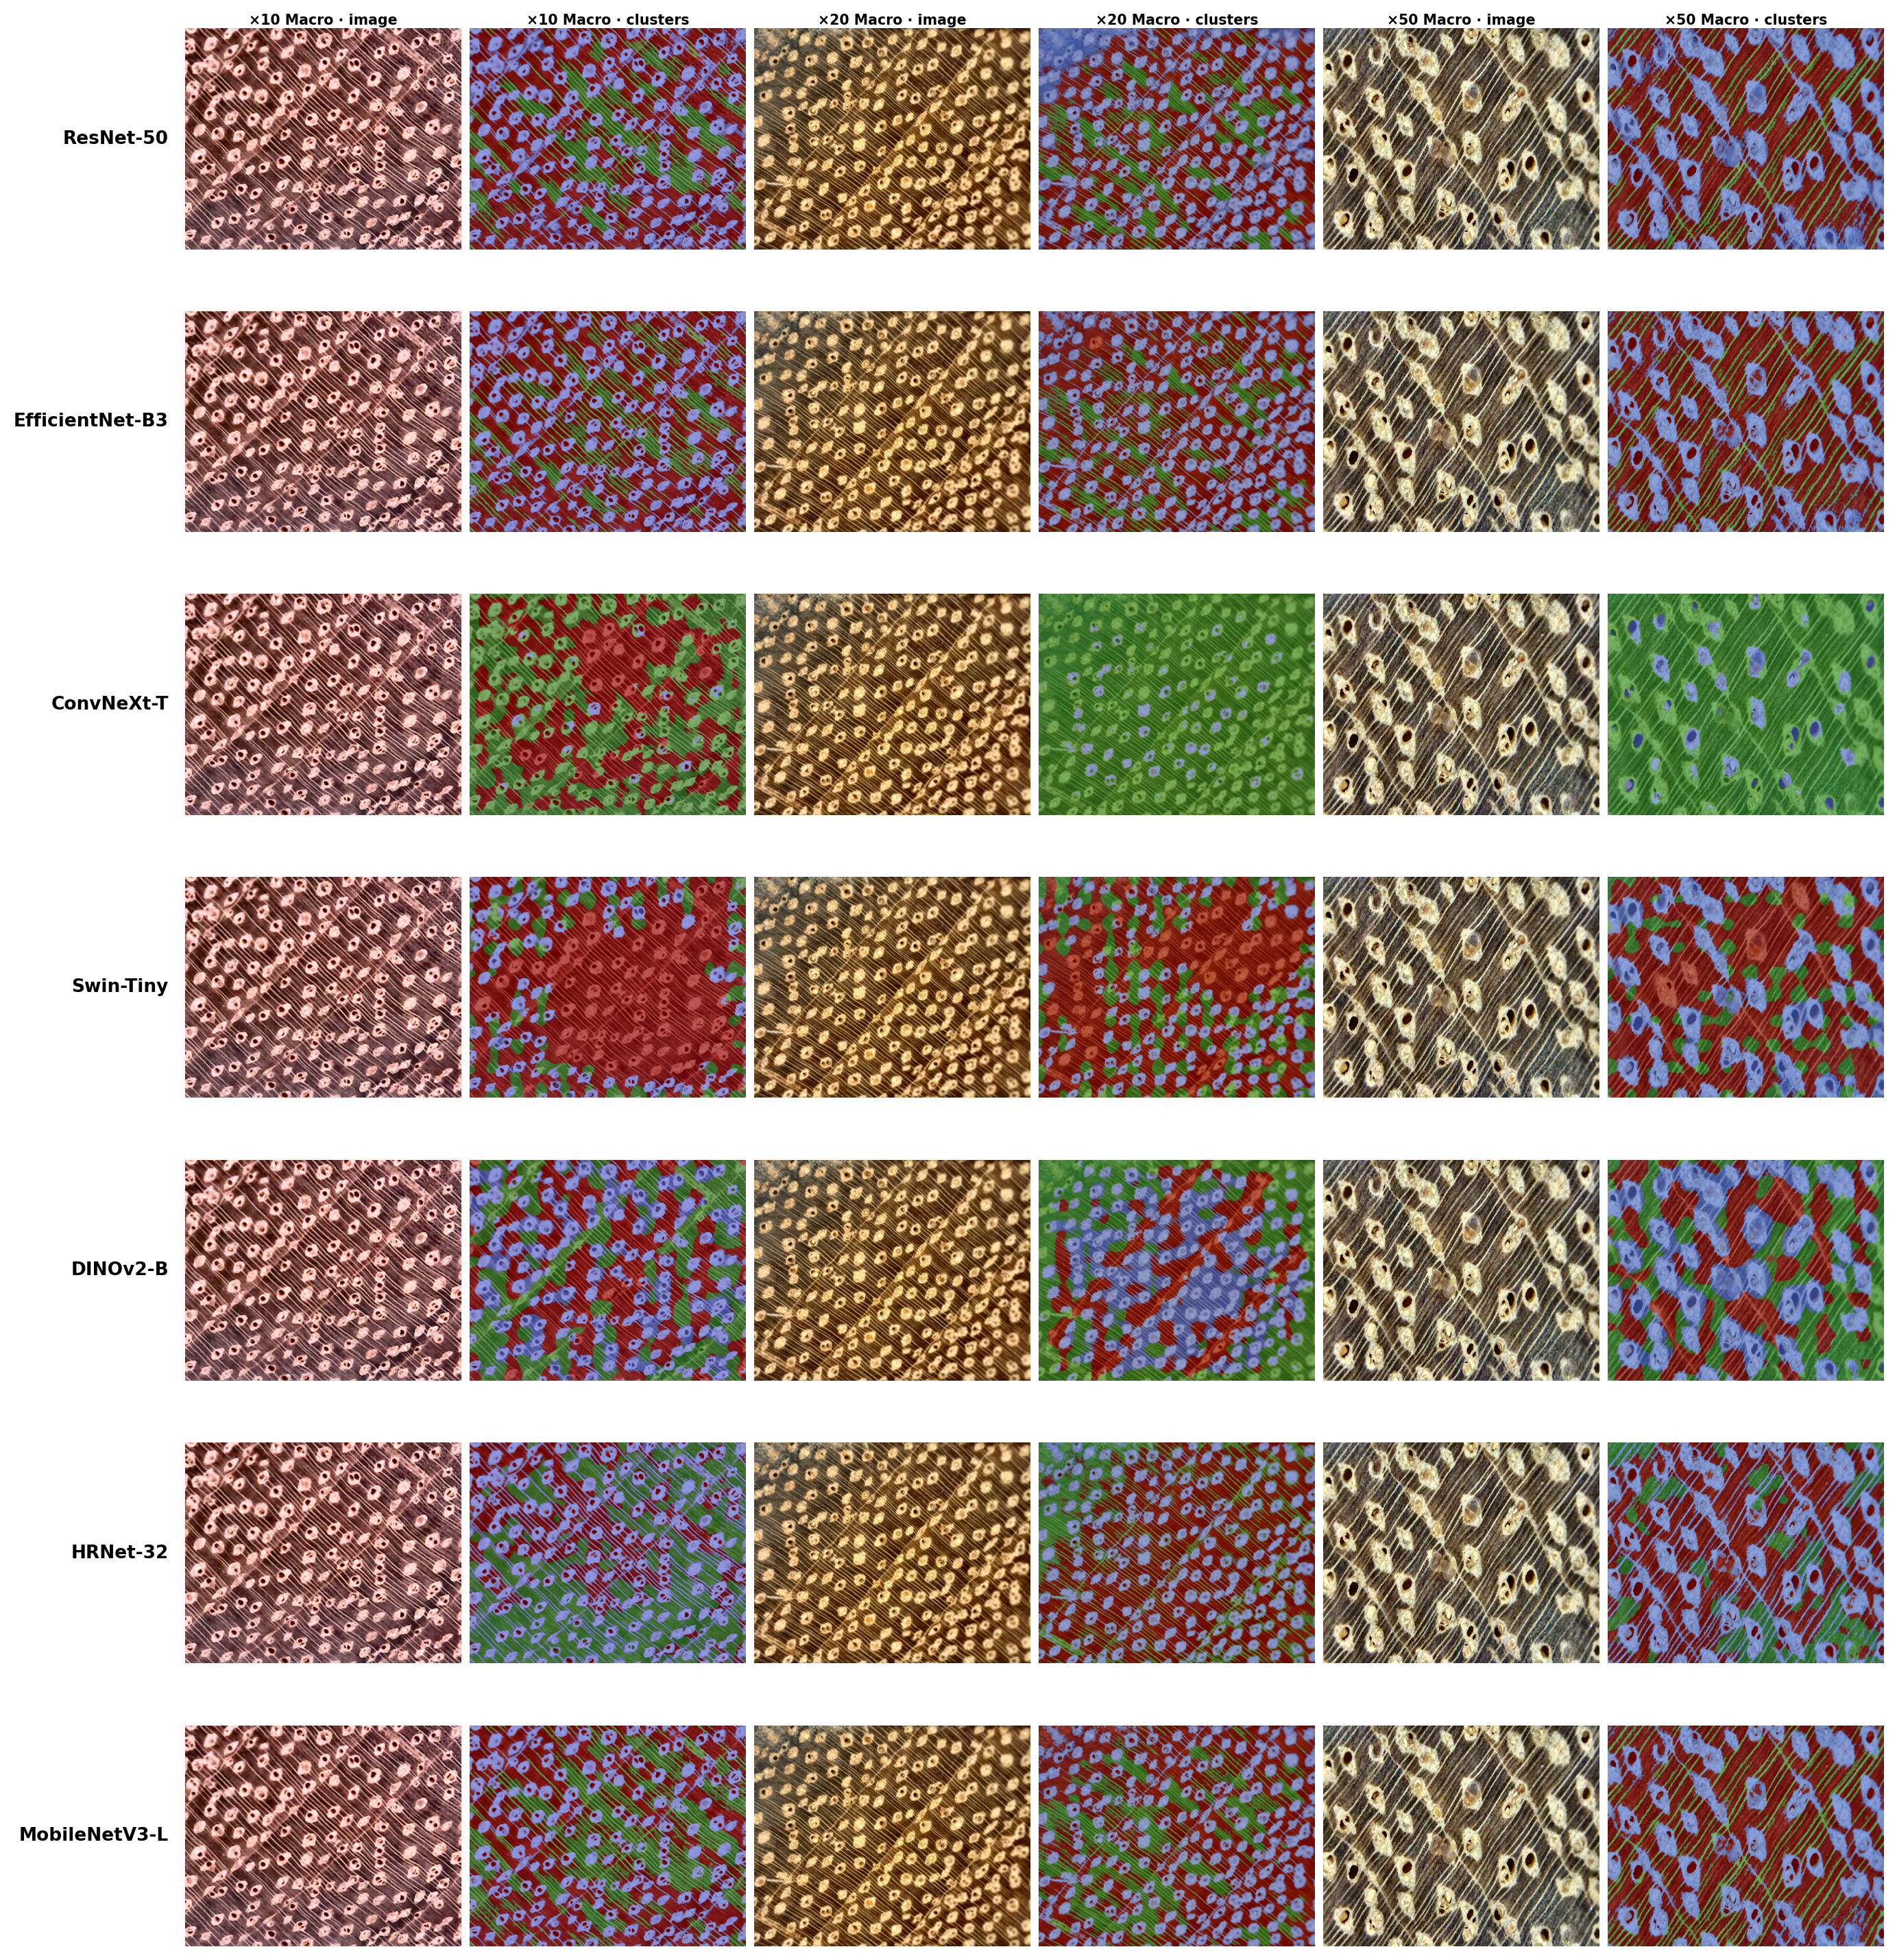
\includegraphics[width=.86\linewidth,height=.52\textheight,keepaspectratio]{results/figures/fig4_spatial_cluster_panels_VN26.png}
\caption{High-resolution VN26 spatial-cluster visualization. These panels are qualitative; quantitative metrics use the standard cached-feature protocol.}
\label{fig:clusters}
\end{figure}

Figure~\ref{fig:vn26_perturb_clusters} gives a complementary perturbation view on VN26 x20. It shows that the cluster overlays are not merely decorative: severe acquisition changes visibly alter local representation partitions, and the pattern of change differs across backbones. This supports the interpretation that SGI and CSI should be used as diagnostic summaries of spatial organization rather than as direct replacements for accuracy or global feature drift.

\begin{figure}[pos=htbp]
\centering
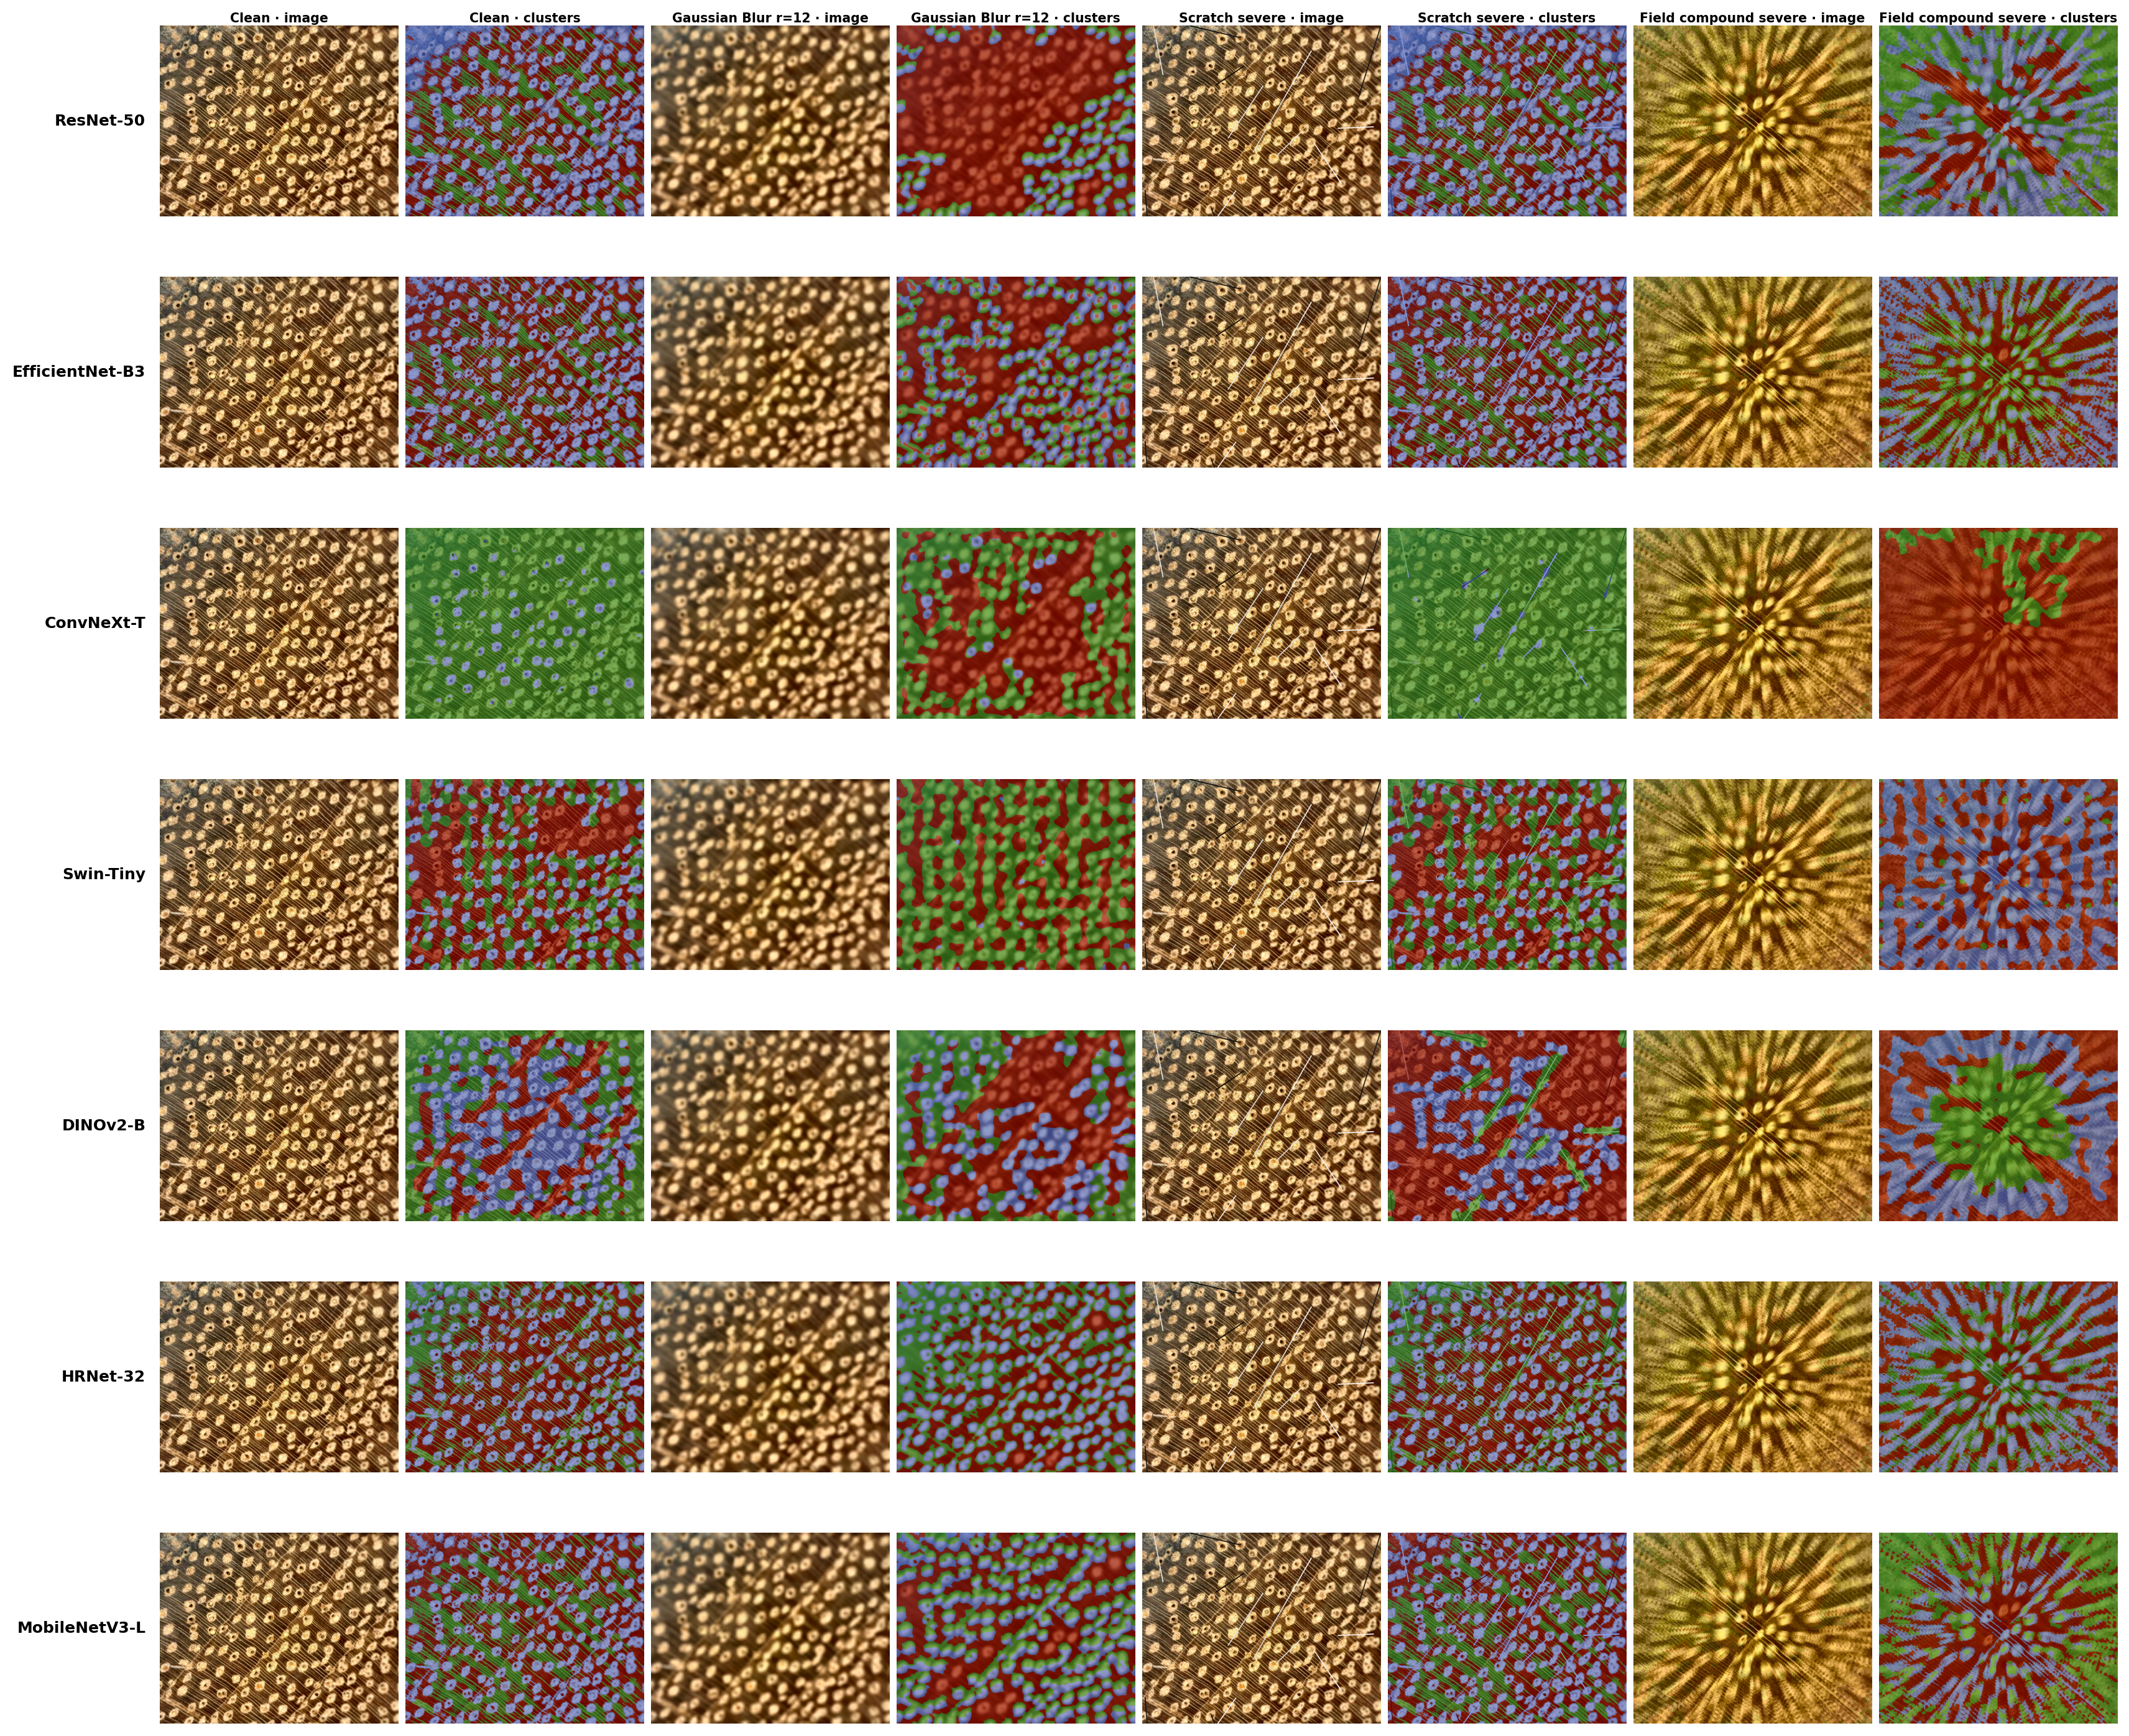
\includegraphics[width=.86\linewidth,height=.52\textheight,keepaspectratio]{results/figures/fig4b_perturbation_VN26x20.png}
\caption{High-resolution VN26 x20 perturbation panels. The visualization compares clean, blurred, and compound-shifted images and their spatial-cluster overlays across backbones.}
\label{fig:vn26_perturb_clusters}
\end{figure}

\begin{figure}[pos=htbp]
\centering
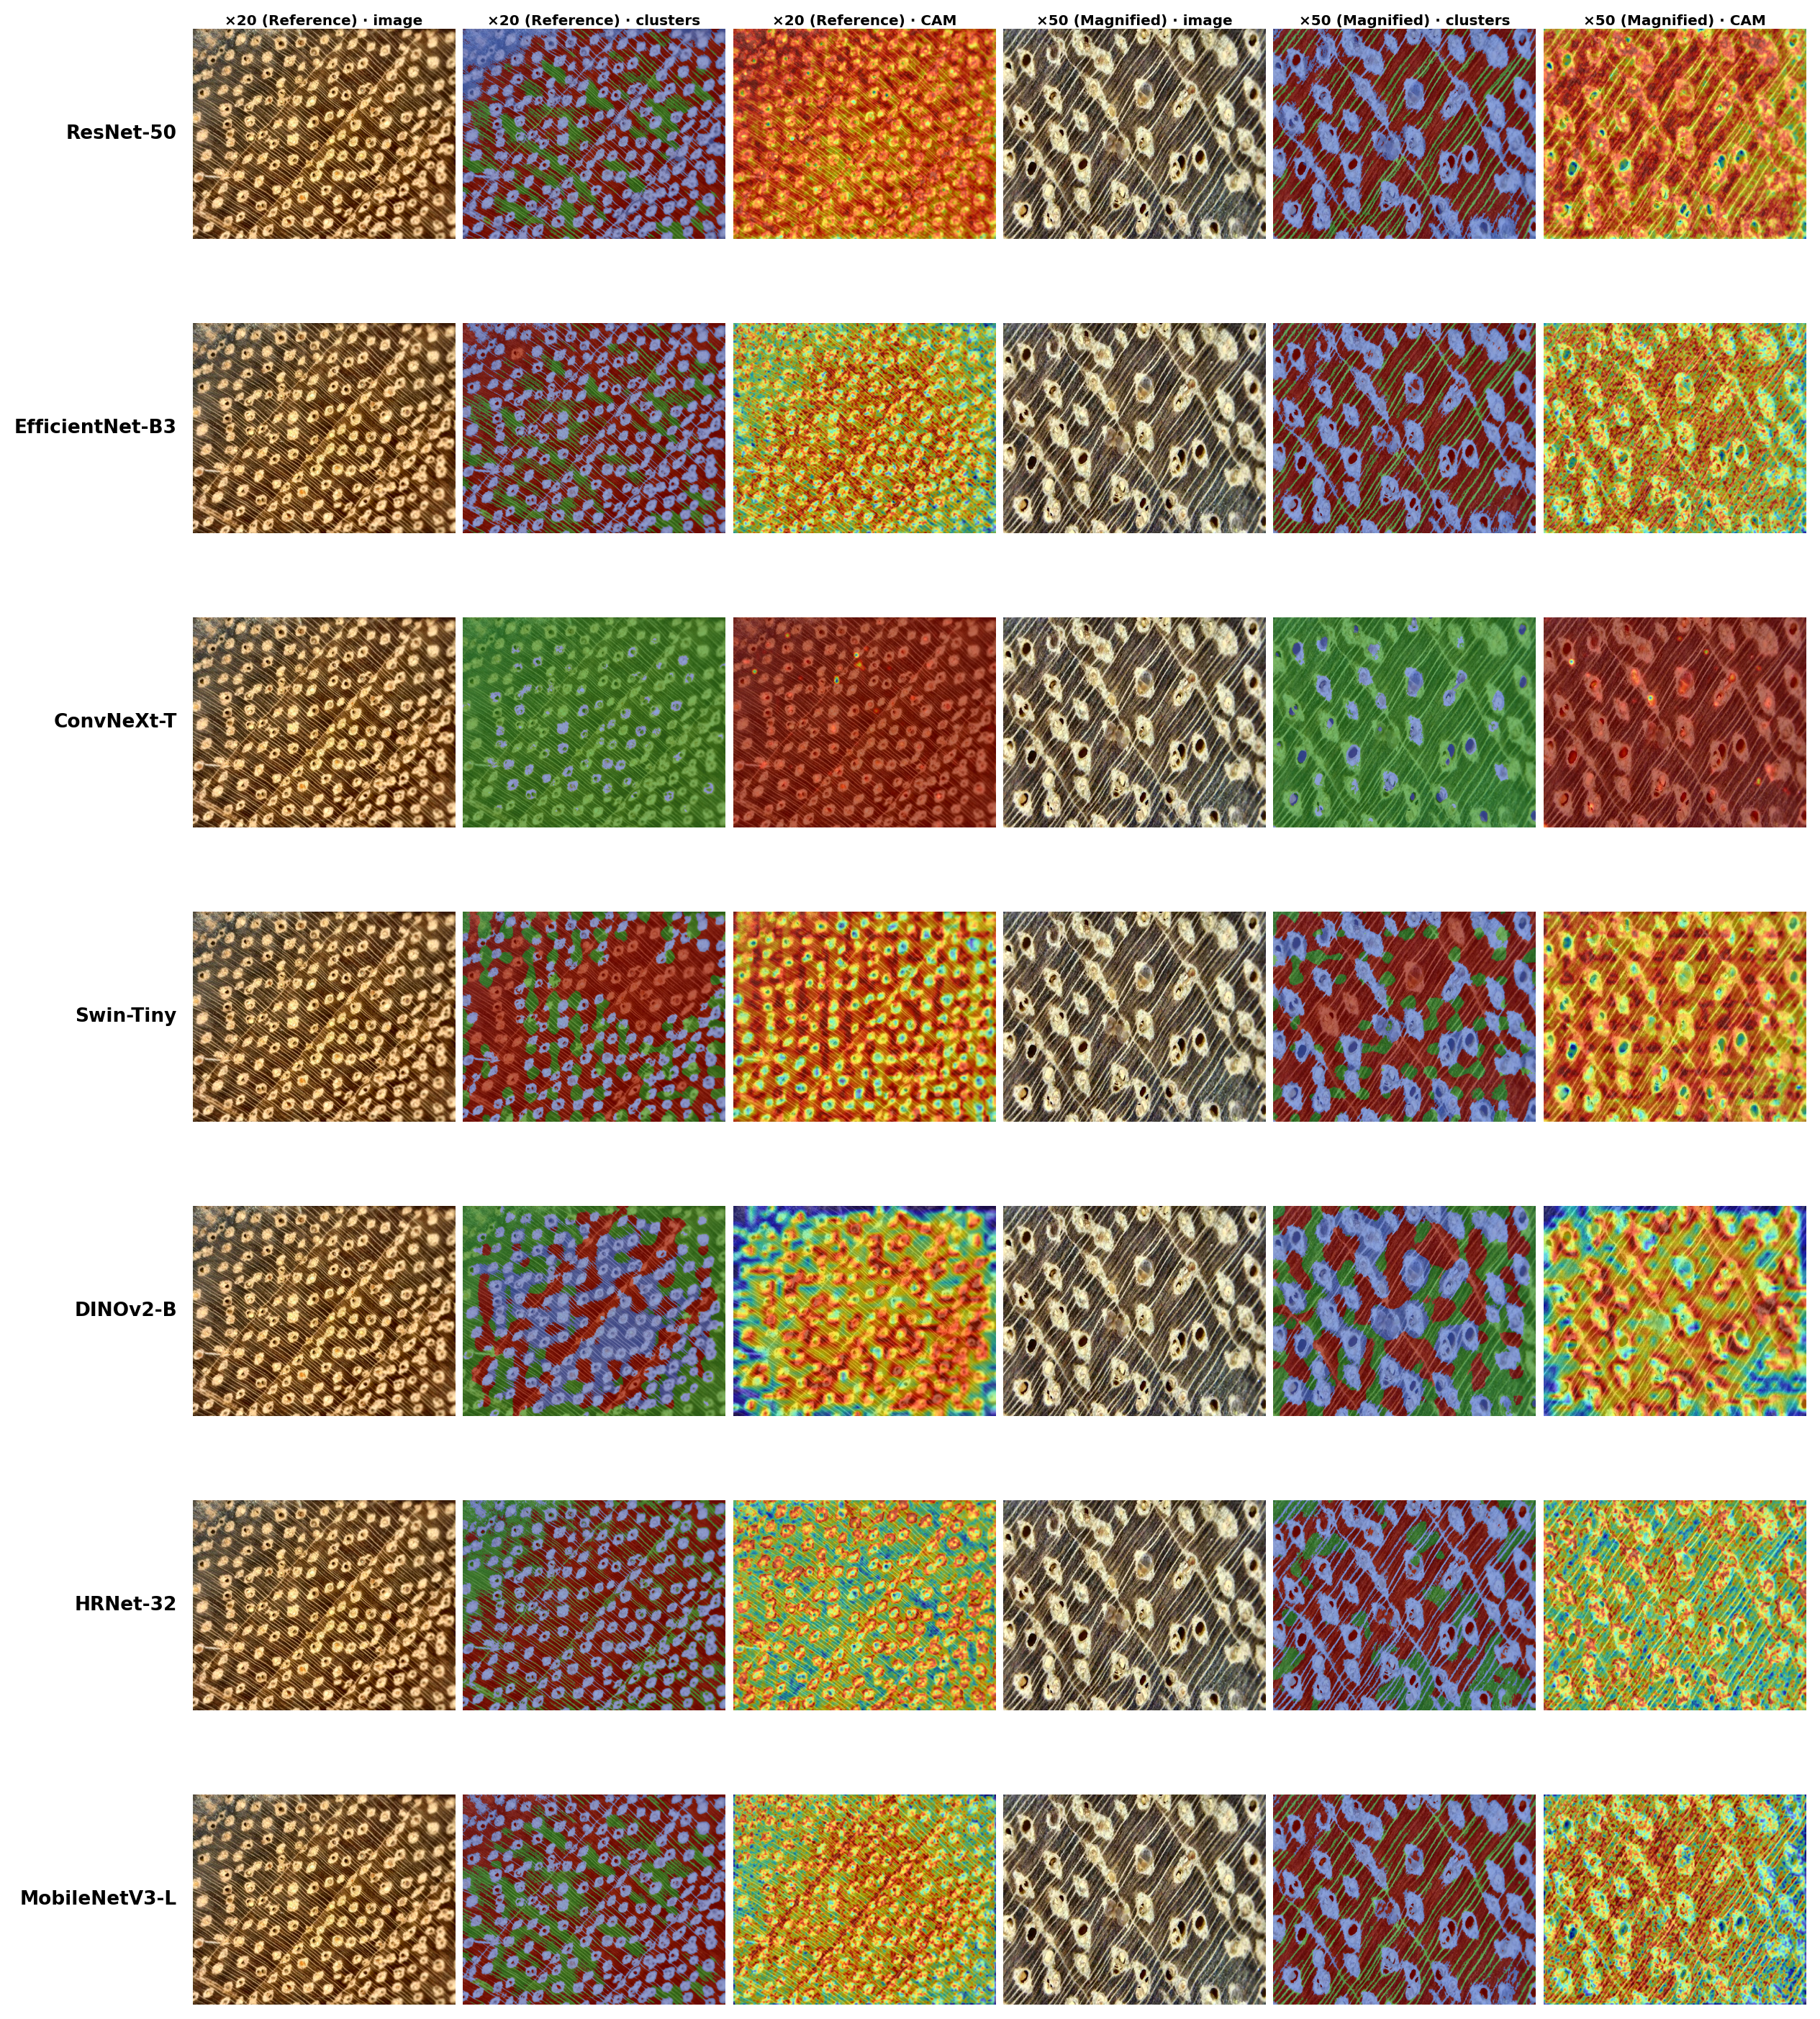
\includegraphics[width=.86\linewidth,height=.52\textheight,keepaspectratio]{results/figures/fig6_cam_cluster_overlay_VN26.png}
\caption{High-resolution VN26 CAM-proxy cluster overlay. CAM-proxy maps are explanatory proxies rather than causal evidence.}
\label{fig:cam_overlay}
\end{figure}

\begin{figure}[pos=htbp]
\centering
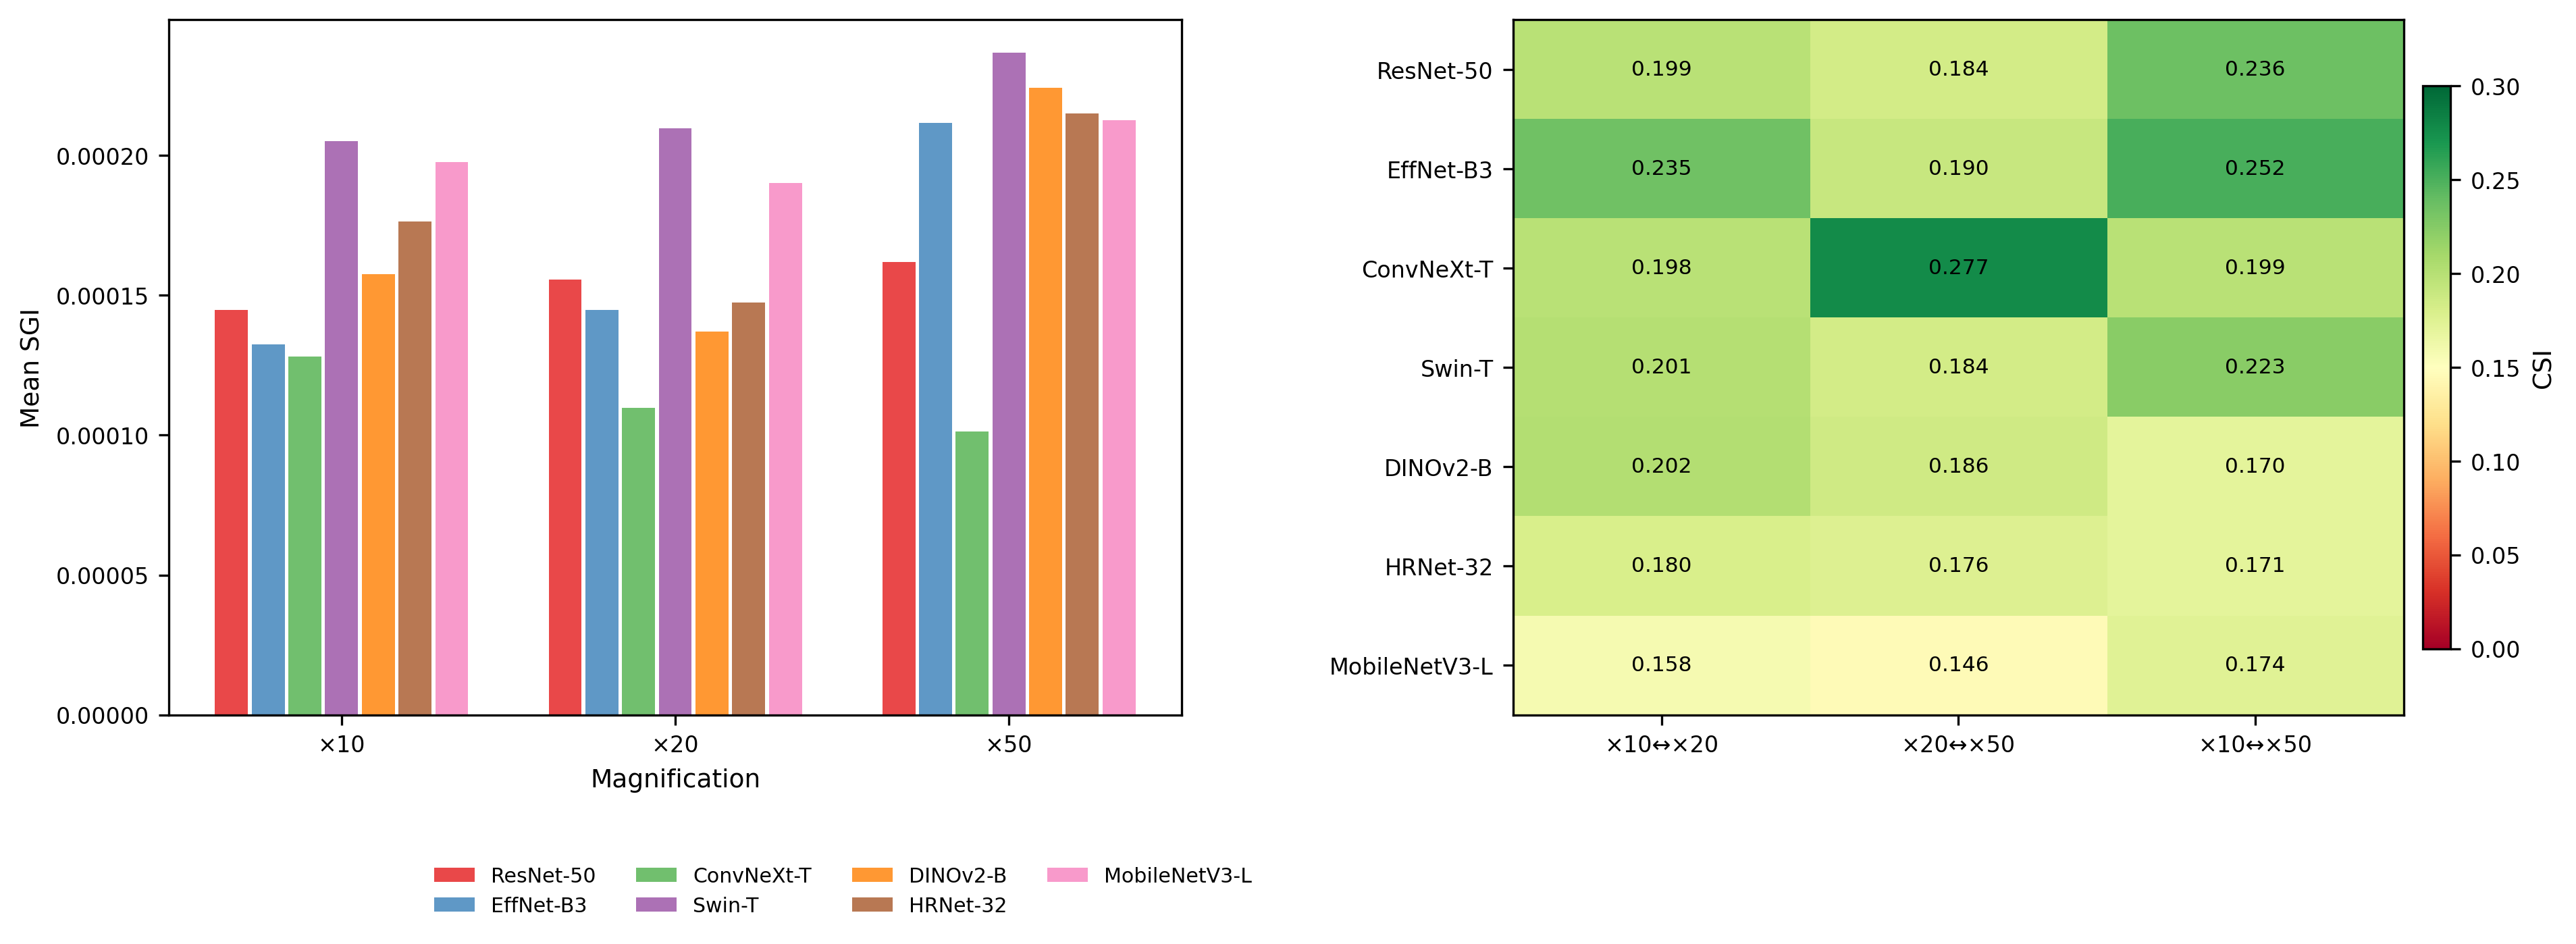
\includegraphics[width=\linewidth]{results/figures/fig12_crossmag_spatial.png}
\caption{Cross-magnification spatial analysis on VN26.}
\label{fig:crossmag}
\end{figure}

Figure~\ref{fig:cam_overlay} visualizes where the CAM-proxy mass concentrates over the representation-derived clusters; the overlay should be read as a diagnostic allocation map, not as causal anatomical attribution. Figure~\ref{fig:crossmag} shows the corresponding cross-magnification spatial analysis, illustrating that spatial organization changes when the same species set is evaluated at different acquisition scales.

Figure~\ref{fig:multilevel_corr_appendix} expands the multilevel diagnostic view behind the main hierarchical model. It shows that spatial instability and CAM-proxy redistribution correlate with accuracy drop, but remain weaker and less direct than paired feature drift. Figures~\ref{fig:csi_drop_appendix}, \ref{fig:cam_shift_drop_appendix}, and~\ref{fig:cam_distribution_appendix} provide the corresponding spatial and CAM-proxy views. These plots support the interpretation used in the main text: spatial and attention-level signals are useful for inspecting failure modes, while global feature displacement remains the most compact quantitative predictor.

\begin{figure}[pos=htbp]
\centering
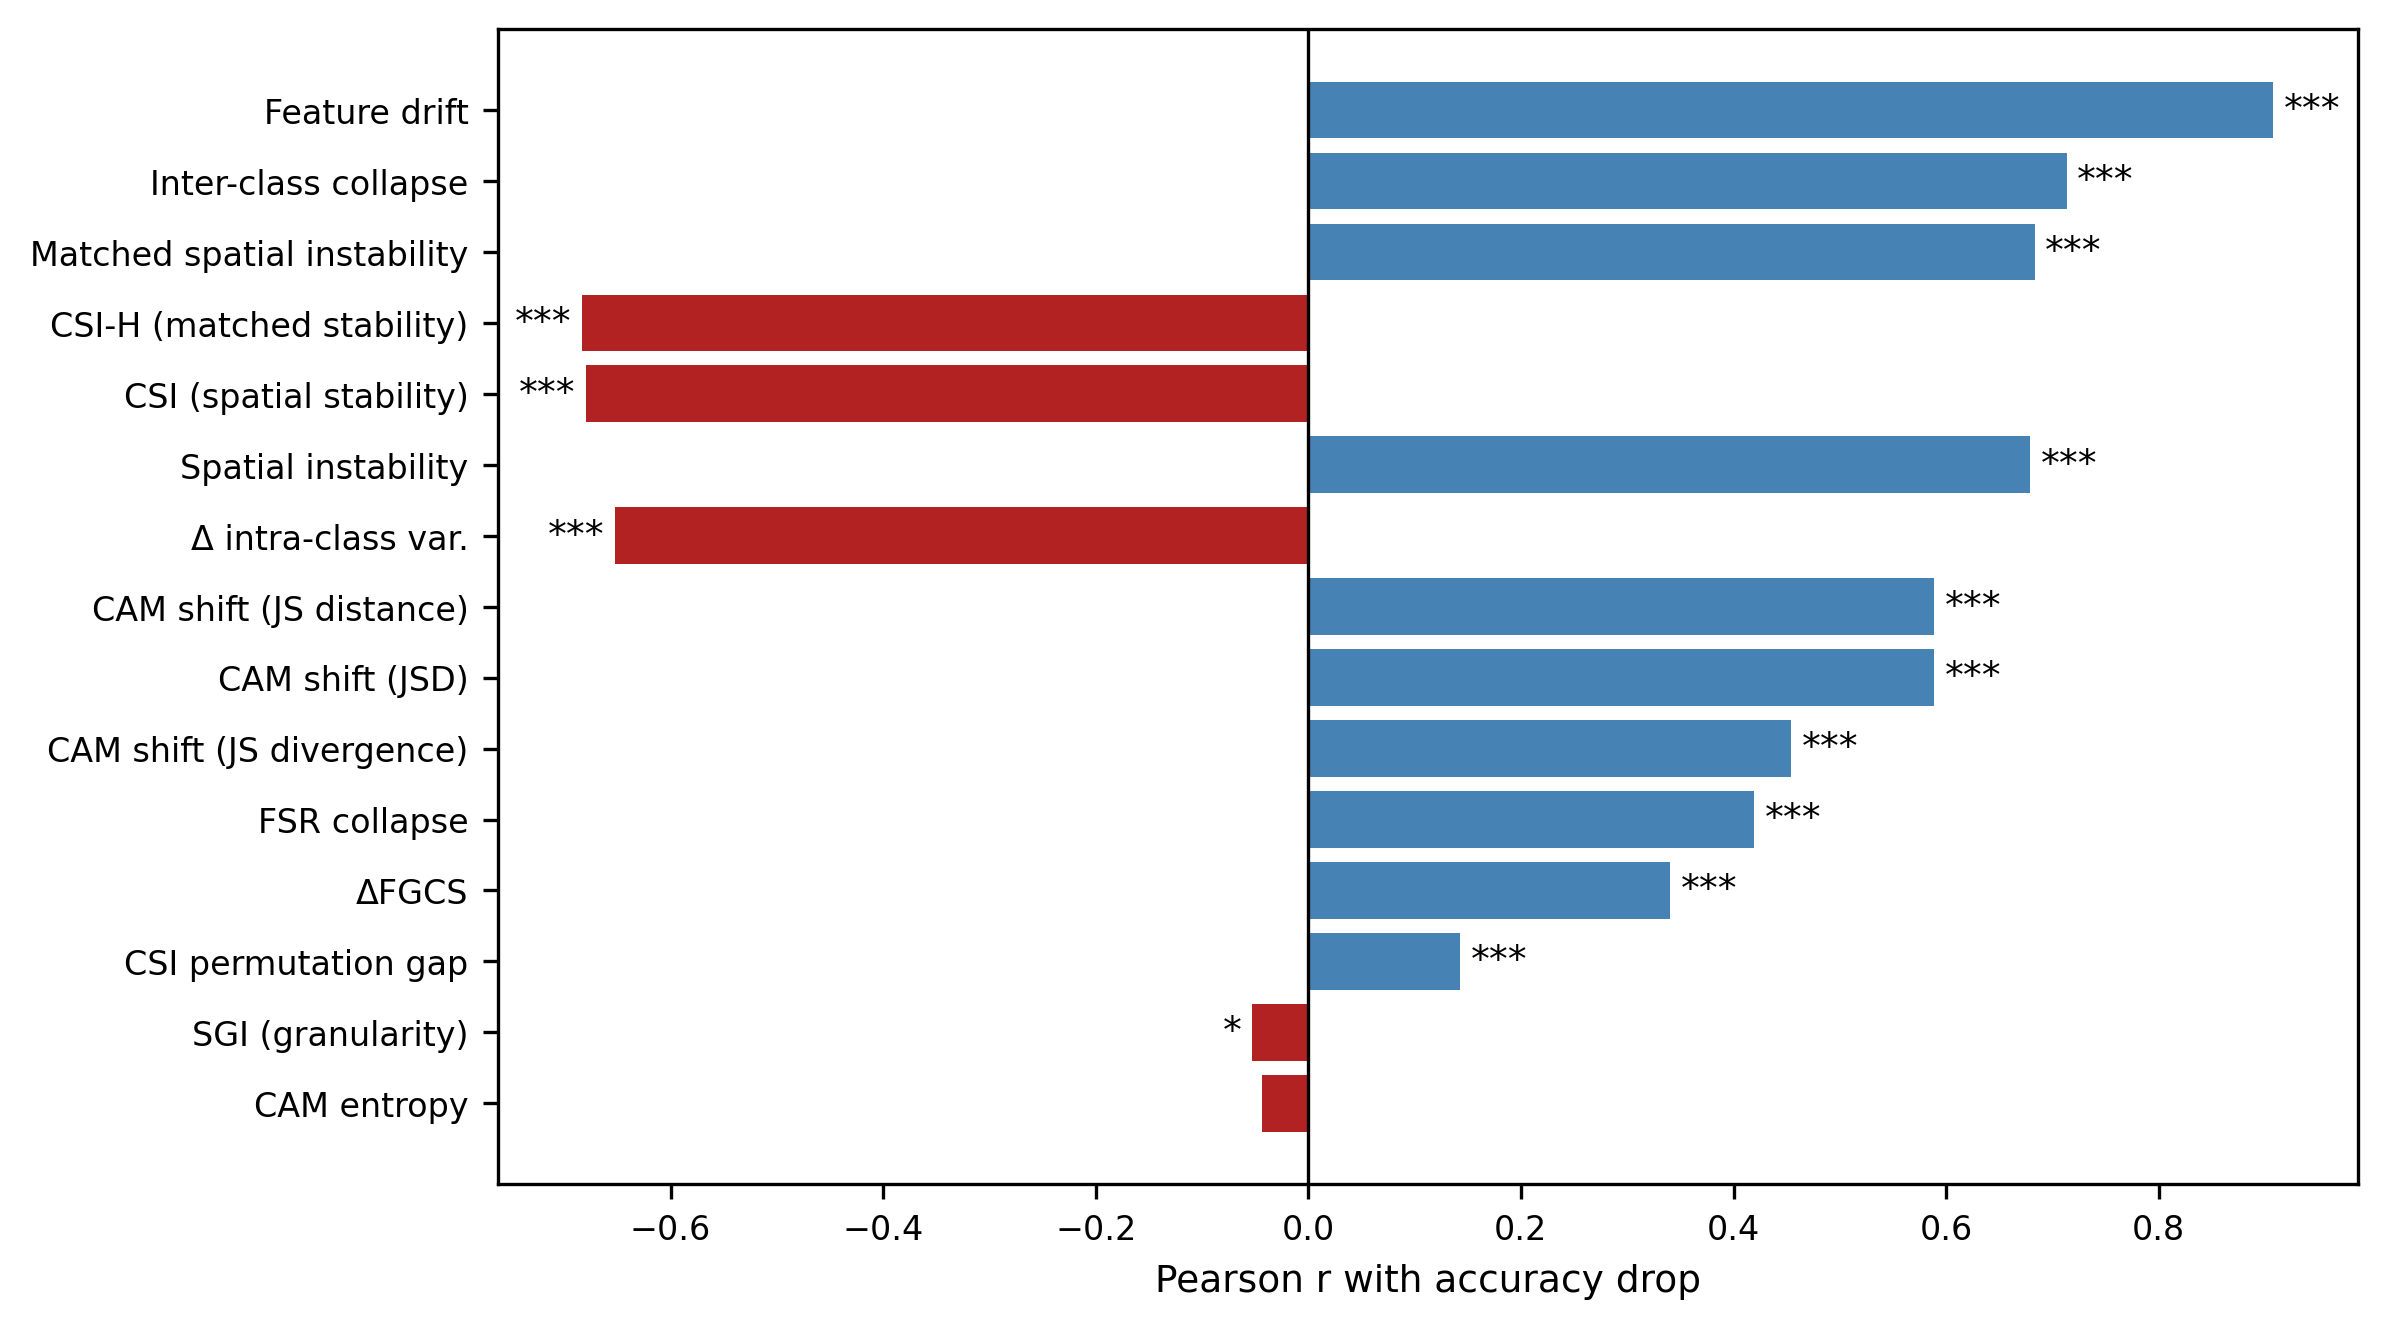
\includegraphics[width=\linewidth]{results/figures/fig_multilevel_correlations.png}
\caption{Additional multilevel correlation summary. Feature drift is the strongest global signal, while spatial and CAM-proxy metrics provide secondary diagnostic information.}
\label{fig:multilevel_corr_appendix}
\end{figure}

\begin{figure}[pos=htbp]
\centering
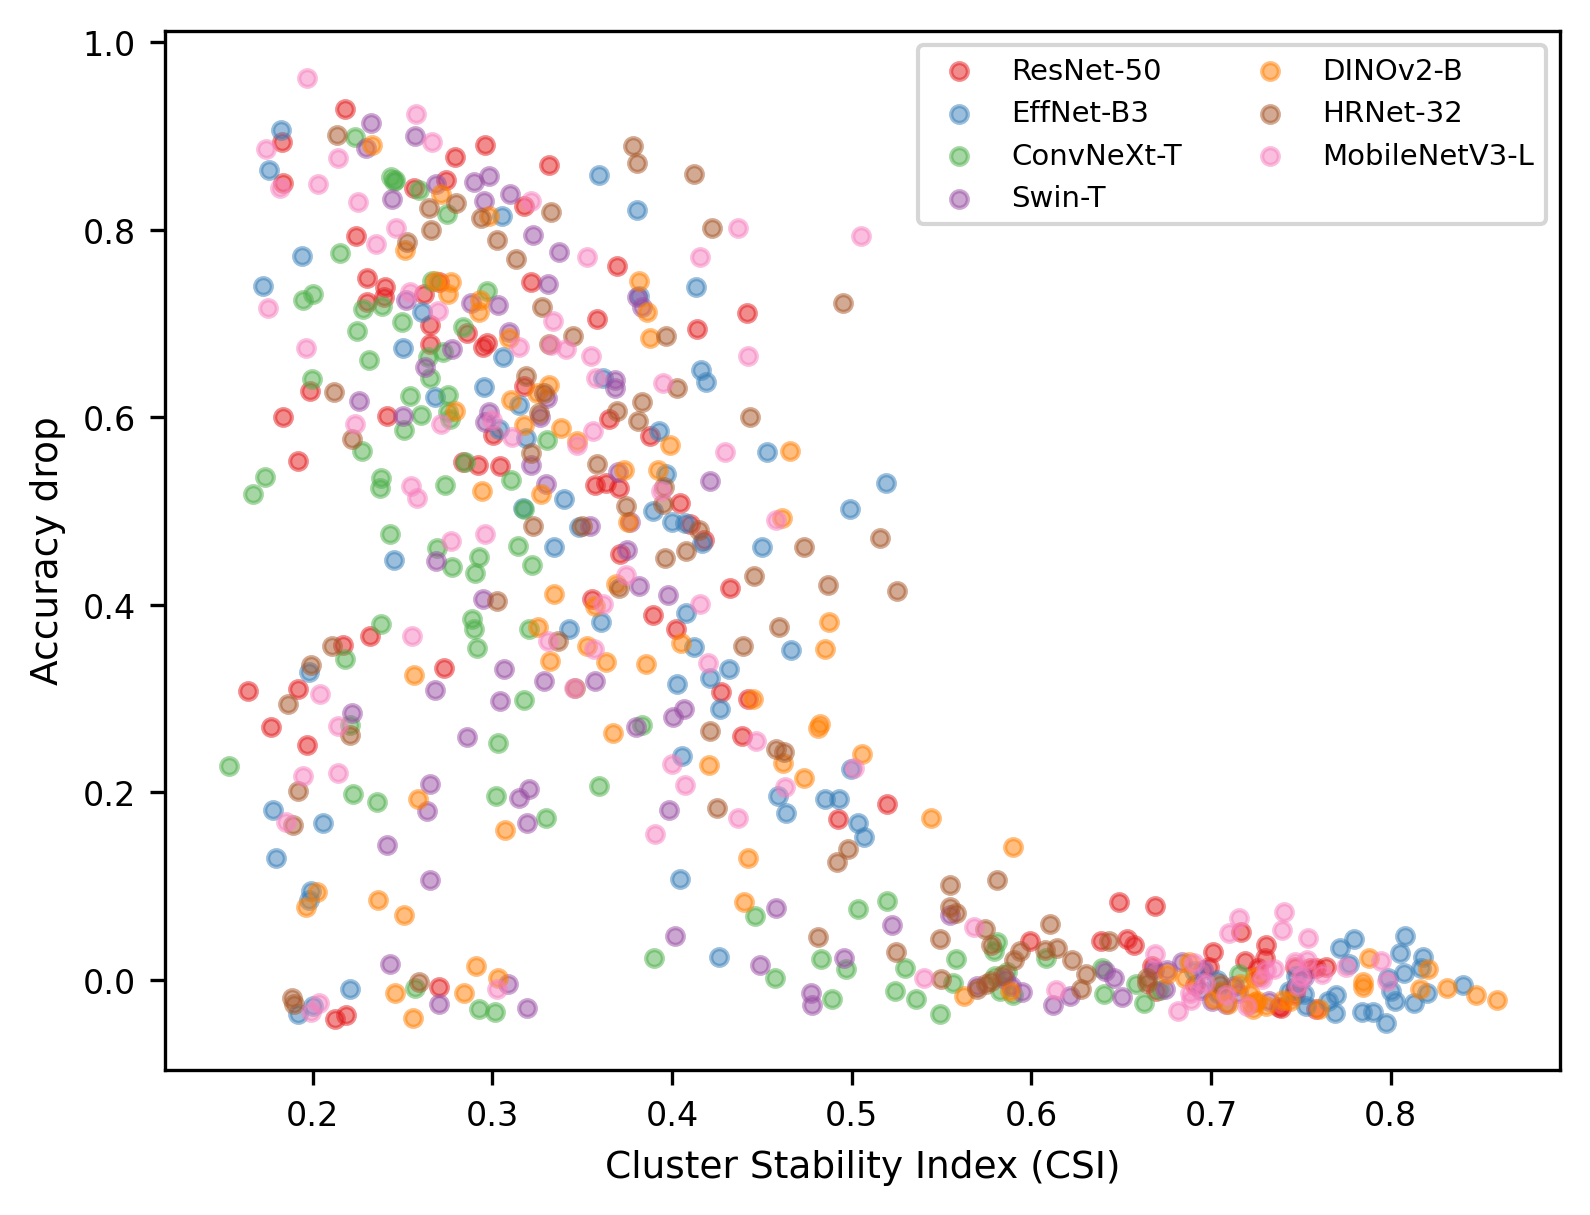
\includegraphics[width=\linewidth]{results/figures/fig_csi_vs_drop.png}
\caption{Spatial cluster stability versus accuracy drop. Lower CSI indicates less stable spatial organization under shift.}
\label{fig:csi_drop_appendix}
\end{figure}

\begin{figure}[pos=htbp]
\centering
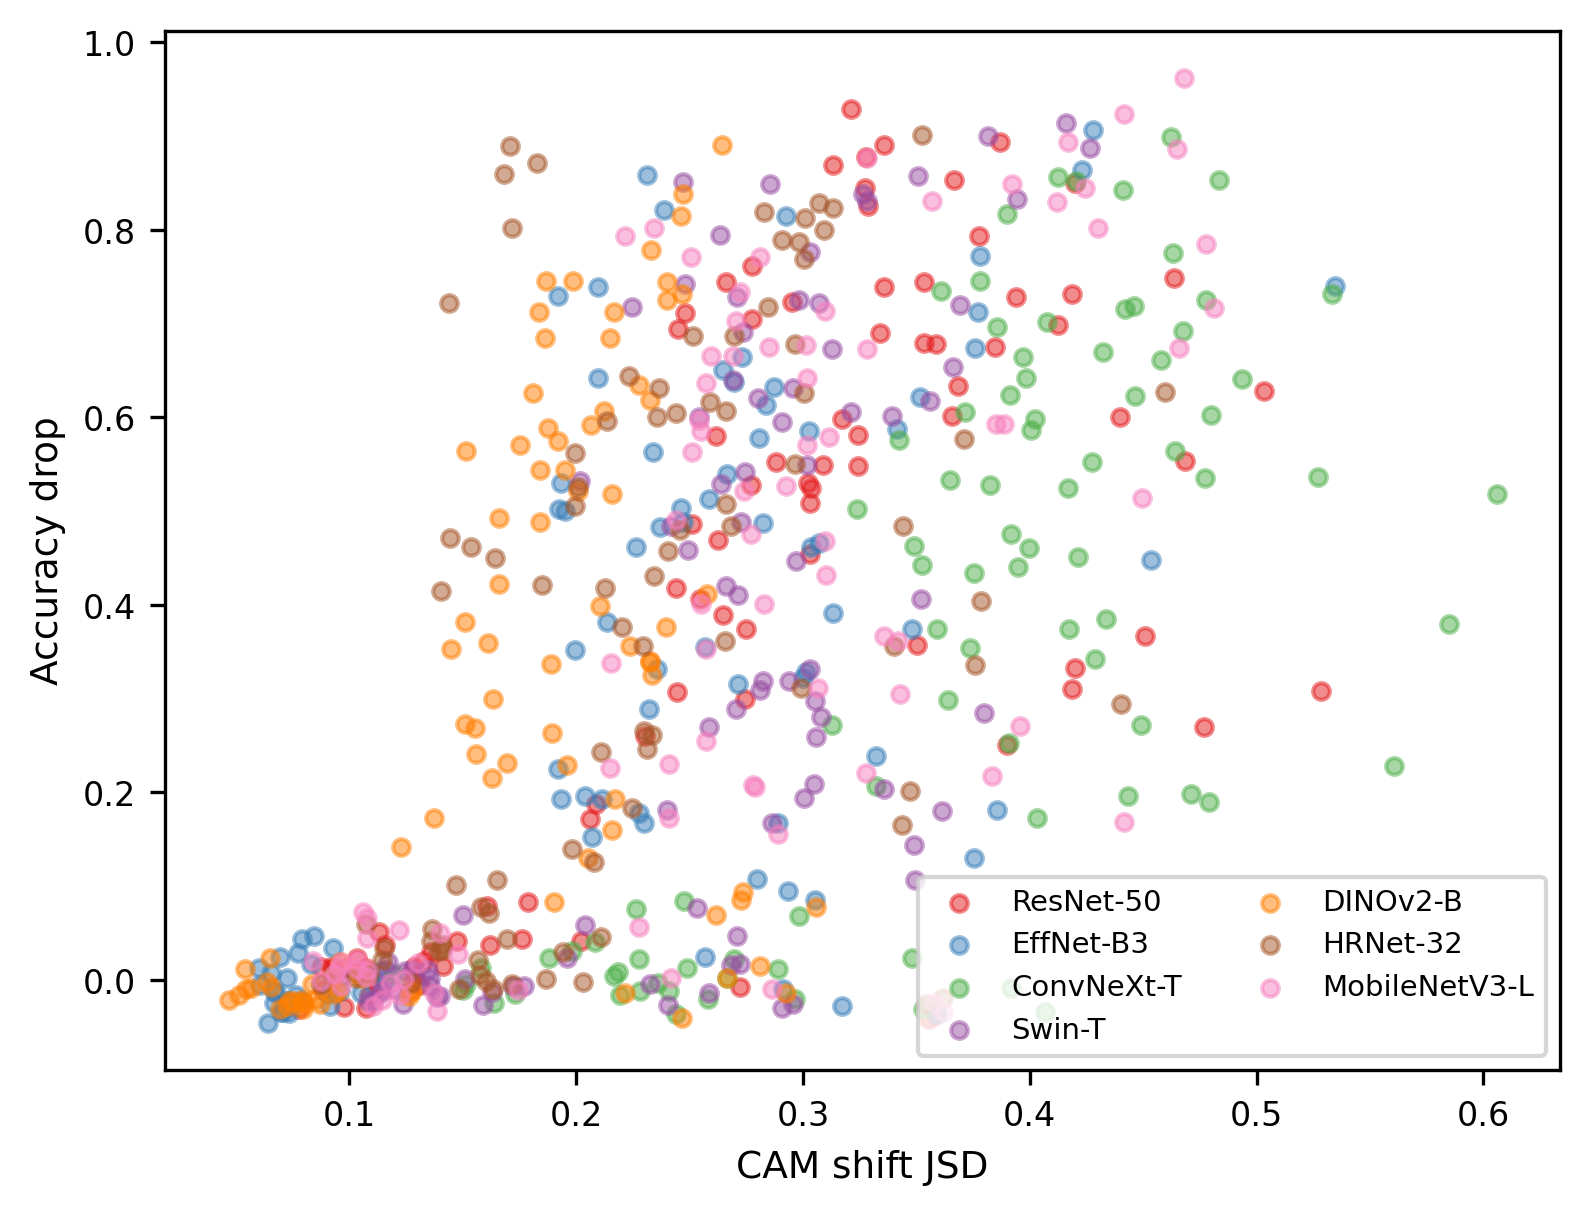
\includegraphics[width=\linewidth]{results/figures/fig_cam_shift_vs_drop.png}
\caption{CAM-proxy cluster redistribution versus accuracy drop. CAM-proxy redistribution is informative but weaker than global feature drift.}
\label{fig:cam_shift_drop_appendix}
\end{figure}

\begin{figure}[pos=htbp]
\centering
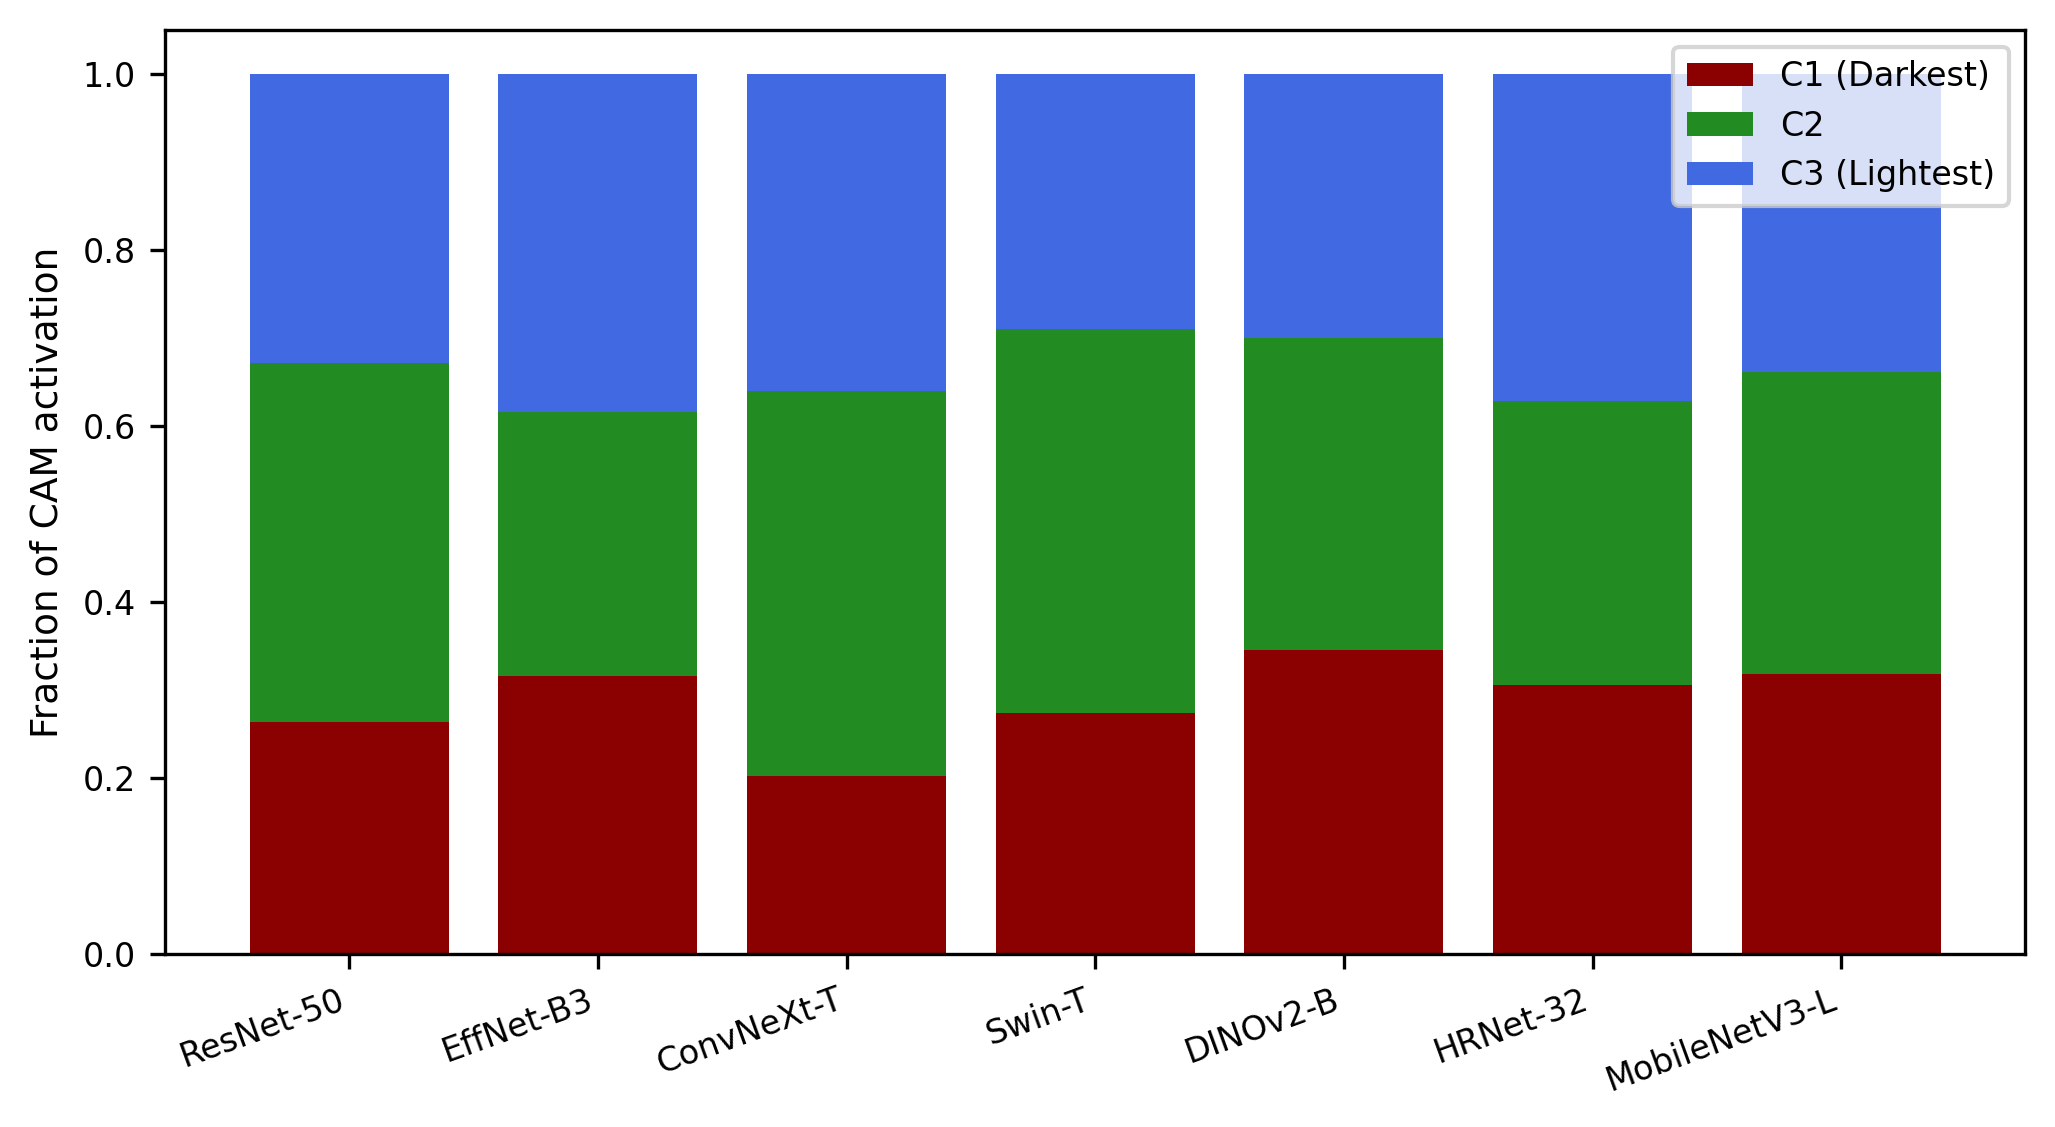
\includegraphics[width=\linewidth]{results/figures/fig_cam_distribution_bars.png}
\caption{CAM-proxy mass distribution over representation-derived spatial clusters. The cluster labels are diagnostic regions, not anatomical annotations.}
\label{fig:cam_distribution_appendix}
\end{figure}

\FloatBarrier
\section{Additional Statistical and Monitoring Checks}
\label{app:additional_checks}

This appendix reports additional statistical and monitoring analyses that support the main claims. Table~\ref{tab:hier_strict} repeats the hierarchical analysis under a stricter complete-case setting where dataset, backbone, perturbation family, and severity are included before any representation metric is added. The increments are smaller than in the main variance-partitioning table because the base controls are already strong. This is expected: dataset identity, backbone identity, perturbation family, and severity are experimental metadata, not operational failure signals available for an incoming unlabeled batch. Representation drift remains the measurable diagnostic quantity that links shift to monitoring, and each representation block still adds non-negative explanatory value beyond the metadata controls. Table~\ref{tab:mmd_oppoints} reports fixed operating points for the RBF-MMD monitor, complementing the ROC-AUC and best-F1 results in the main text. Tables~\ref{tab:lopo} and~\ref{tab:batch_ref} report leave-one-perturbation-family-out and batch/reference-bank sensitivity checks. Table~\ref{tab:decision_rule} checks whether the main feature-drift conclusion depends on the chosen frozen-feature decision rule. The frozen linear-probe row is especially useful for the circularity check: the probe is a multinomial logistic regression trained on clean training-split features and evaluated on perturbed test-split features, so it does not match a query to its own clean embedding. Despite replacing nearest-neighbour voting with this non-kNN classifier, feature drift remains strongly associated with accuracy drop ($r=0.922$, $\rho=0.942$, $n=1596$).

\begin{table}[pos=htbp]
\centering
\caption{Representative quantitative context from prior WoodID studies. Reported values are taken from the corresponding papers and are not directly comparable because protocols differ.}
\label{tab:related_quant}
\footnotesize
\begin{tabular}{p{0.27\linewidth}p{0.31\linewidth}p{0.30\linewidth}}
\toprule
Study & Setting & Reported result and relevance \\
\midrule
\citet{paulafilho2014forest} & Macroscopic Brazilian forest species, divide-and-conquer descriptors & 97.77\% best recognition rate on 41 species; strong controlled macroscopic benchmark. \\
\citet{souza2020brazilian} & LBP texture descriptors and classifier fusion on 46 Brazilian species & 97.67\% F1-score, improved by 0.33 percentage points with majority voting. \\
\citet{sun2021smallwood} & ResNet50--LDA--KNN on 25 rare wood species & 0.996 testing accuracy and 0.994 F1-score; explicitly discusses generalization to new samples. \\
\citet{fabijanska2021woodcore} & Residual CNN with patch voting on wood-core images & 93\% patch-level accuracy and 98.7\% wood-core accuracy. \\
\citet{degeus2021amazon} & Amazon wood classification after simplified pocket-knife surface preparation & 98.13\% accuracy with DenseNet; moves acquisition closer to field use. \\
\citet{barmpoutis2018woodauth} & Multi-section texture analysis for Greek wood species & 91.47\% on cross sections and 84.2\% with multiple section types. \\
\citet{herrera2026goimai} & High-resolution patch-voting on GOIMAI-Phase-I & 99.4\% accuracy; highlights the value of high-resolution local detail. \\
\citet{ravindran2021field} & Field-deployable XyloTron system for Peruvian timbers & 86.5\% top-1 specimen-level accuracy; demonstrates operational WoodID relevance. \\
\citet{owens2025robustness} & Perturbation robustness of a Peruvian WoodID model & 89.2\% unperturbed baseline; blue-channel shift, resizing, and large blur perturbations can cause substantial accuracy losses in their model. \\
\bottomrule
\end{tabular}
\end{table}

\begin{table}[pos=htbp]
\centering
\caption{Controlled complete-case hierarchical regression. The base model includes dataset, backbone, perturbation family, and severity controls before adding representation metrics.}
\label{tab:hier_strict}
\small
\begin{tabular}{lcc}
\toprule
Model & $R^2$ & $\Delta R^2$ \\
\midrule
Controls only & 0.897 & 0.897 \\
+ Feature drift & 0.929 & 0.031 \\
+ Feature geometry & 0.937 & 0.008 \\
+ Spatial metrics & 0.938 & 0.001 \\
+ CAM-proxy metrics & 0.938 & 0.000 \\
\bottomrule
\end{tabular}
\end{table}

\begin{table}[pos=htbp]
\centering
\caption{Fixed operating points for the RBF-MMD deployment monitor over 4256 records.}
\label{tab:mmd_oppoints}
\small
\begin{tabular}{lcc}
\toprule
Operating point & Value & Threshold \\
\midrule
TPR at FPR = 0.05 & 0.810 & 0.112 \\
TPR at FPR = 0.10 & 0.908 & 0.083 \\
FPR at TPR = 0.90 & 0.093 & 0.086 \\
FPR at TPR = 0.95 & 0.152 & 0.066 \\
\bottomrule
\end{tabular}
\end{table}

\begin{table}[pos=htbp]
\centering
\caption{Leave-one-perturbation-family-out evaluation for the RBF-MMD reference-bank monitor. Selected held-out families are shown; AUC is undefined when the held-out family contains only one failure class. Rows with failure rate 0 or 1 are threshold-behavior checks rather than discriminative-performance estimates.}
\label{tab:lopo}
\small
\begin{tabular}{lcccc}
\toprule
Held-out family & Failure rate & ROC-AUC & F1 & FPR \\
\midrule
Gaussian blur & 0.920 & 0.983 & 0.981 & 0.259 \\
Defocus blur & 0.879 & 0.967 & 0.965 & 0.235 \\
Rotation & 0.429 & 0.974 & 0.923 & 0.125 \\
JPEG & 0.304 & 0.911 & 0.687 & 0.338 \\
Resize & 0.196 & 0.866 & 0.481 & 0.059 \\
Red-channel shift & 0.022 & 0.944 & 0.000 & 0.009 \\
Blue-channel shift & 0.009 & 0.966 & 0.000 & 0.000 \\
Compound & 1.000 & -- & 1.000 & 0.000 \\
Illumination & 0.000 & -- & 0.000 & 0.000 \\
\bottomrule
\end{tabular}
\end{table}

\begin{table}[pos=htbp]
\centering
\caption{RBF-MMD monitor sensitivity to deployment batch size and clean reference-bank size. Entries are ROC-AUC values. Reference-bank size is capped by available clean samples, hence the BD11-limited 440-sample setting.}
\label{tab:batch_ref}
\small
\begin{tabular}{lccccc}
\toprule
Batch size & Ref. 100 & Ref. 250 & Ref. 440 & Ref. 500 & Ref. 1000 \\
\midrule
8  & 0.924 & 0.926 & 0.927 & 0.930 & 0.928 \\
16 & 0.950 & 0.950 & 0.959 & 0.953 & 0.954 \\
32 & 0.961 & 0.961 & 0.972 & 0.963 & 0.964 \\
64 & 0.964 & 0.965 & 0.977 & 0.967 & 0.967 \\
\bottomrule
\end{tabular}
\end{table}

\begin{table}[pos=htbp]
\centering
\caption{Decision-rule sensitivity for frozen-feature evaluation. Values are averaged over Tier-A perturbation records. The main feature-drift conclusion remains stable for kNN-1/3/5/10; nearest-centroid classification is less accurate but still preserves a strong drift/drop association.}
\label{tab:decision_rule}
\small
\begin{tabular}{lcccc}
\toprule
Decision rule & Clean acc. & Pert. acc. & Pearson $r$ & Spearman $\rho$ \\
\midrule
kNN-1 & 0.948 & 0.701 & 0.916 & 0.928 \\
kNN-3 & 0.945 & 0.688 & 0.911 & 0.937 \\
kNN-5 & 0.942 & 0.685 & 0.908 & 0.937 \\
kNN-10 & 0.933 & 0.678 & 0.904 & 0.935 \\
Nearest centroid & 0.802 & 0.567 & 0.880 & 0.908 \\
Linear probe & 0.925 & 0.685 & 0.922 & 0.942 \\
\bottomrule
\end{tabular}
\end{table}

\subsection*{Negative-control deblurring check}

We also ran a negative-control restoration check on Gaussian-blur conditions. This check is not used as a mitigation claim; its purpose is to test whether a visually plausible preprocessing intervention automatically reduces representation drift. The intervention applies frequency-domain Wiener deconvolution using a Gaussian point-spread function estimated from the known blur radius and a fixed noise assumption. The answer is no. Averaged over 126 backbone--dataset--blur-radius records, blurred accuracy is 0.469, while the deblurred output drops to 0.297. Mean paired drift also increases from 0.488 to 0.638. Deblurring improves accuracy in only 10.3\% of records and reduces representation drift in only 8.7\% of records. Table~\ref{tab:deblur} summarizes the result by blur radius. This negative control supports the monitoring argument: acquisition-quality corrections should be validated through representation stability and recognition behavior, rather than assumed to improve robustness.

\begin{table}[pos=htbp]
\centering
\caption{Negative-control deblurring intervention on Gaussian-blur conditions. Values are averaged over datasets and backbones.}
\label{tab:deblur}
\small
\begin{tabular}{lcccc}
\toprule
Blur radius & Blur acc. & Deblur acc. & Blur drift & Deblur drift \\
\midrule
2  & 0.853 & 0.590 & 0.194 & 0.404 \\
4  & 0.616 & 0.412 & 0.366 & 0.566 \\
6  & 0.454 & 0.238 & 0.491 & 0.668 \\
8  & 0.366 & 0.193 & 0.574 & 0.706 \\
10 & 0.282 & 0.182 & 0.631 & 0.733 \\
12 & 0.245 & 0.165 & 0.674 & 0.748 \\
\bottomrule
\end{tabular}
\end{table}

\section*{Data and Code Availability}

Code, configurations, processed results, and figure-generation scripts are publicly available for reproducibility at \url{https://github.com/thanhmcisai/mrd-wood}. Public datasets are used according to their original licenses and cited sources.

\section*{Acknowledgements}

The authors thank the Intelligent Computing for Sustainable Development Lab at the Posts and Telecommunications Institute of Technology (PTIT) for supporting the research environment used in this study.

\clearpage

\bibliographystyle{els-cas-templates/cas-model2-names}
\bibliography{references}

\end{document}
